\documentclass[a4paper,12pt]{report}
%------------- package -----------------------
\usepackage[french]{babel}
\usepackage[T1]{fontenc}
\usepackage{fancyhdr}
\usepackage{inputenc}
\usepackage[top=2cm, bottom=2cm, left=2.5cm, right=2cm]{geometry}
\usepackage{lmodern,tikz,lipsum}
\newcommand\framethispage[1][1cm]{%
    \tikz[overlay,remember picture,line width=2.5pt]
    \draw([xshift=(#1),yshift=(-#1)]current page.north west)rectangle
         ([xshift=(-#1),yshift=(#1)]current page.south east);%
}
\usepackage{xcolor}
\usepackage{float}
\usepackage{lmodern}
\usepackage{amsmath}
\usepackage{amssymb}
\usepackage{graphicx}
\usepackage[colorinlistoftodos]{todonotes}
\usepackage{url}
\usepackage{hyperref}
\usepackage{array}
\usepackage{tabularx}
\usepackage{setspace}
\usepackage{abstract}
\usepackage{subfig}
\usepackage{layout}
\usepackage{ragged2e}

% Tikz for graphs
\usepackage{tikz}
\usetikzlibrary{shapes.geometric, arrows.meta, positioning, fit}

% Code Box (morceaux du codes)
\usepackage{float}
\usepackage{xcolor}
\usepackage{graphicx}
\usepackage{caption}
\usepackage{listings}
\usepackage[most]{tcolorbox}

\definecolor{codebg}{RGB}{245,245,244}
\definecolor{codeframe}{RGB}{210,210,210}
\definecolor{codecomment}{RGB}{0,128,0}
\definecolor{codekeyword}{RGB}{0,0,180}
\definecolor{codestring}{RGB}{163,21,21}

\lstdefinestyle{sonacode}{
    backgroundcolor=\color{codebg},
    frame=single,
    rulecolor=\color{codeframe},
    basicstyle=\ttfamily\small,
    keywordstyle=\color{codekeyword}\bfseries,
    commentstyle=\color{codecomment},
    stringstyle=\color{codestring},
    breaklines=true,
    showstringspaces=false,
    tabsize=2,
    captionpos=b
}


\renewcommand{\thechapter}{\Roman{chapter}}

\definecolor{bleu}{RGB}{0,76,153}
\definecolor{bleuu}{RGB}{0,102,204}

\makeatletter
\def\headrule{{\if@fancyplain\let\headrulewidth\plainheadrulewidth\fi
		\color{bleu}\hrule\@height\headrulewidth\@width\headwidth \vskip-\headrulewidth}}
\def\footrule{{\if@fancyplain\let\footrulewidth\plainfootrulewidth\fi
		\vskip-\footruleskip\vskip-\footrulewidth
		\color{bleu}\color{bleu}\hrule\@width\headwidth\@height\footrulewidth\vskip\footruleskip}}
\makeatother


%------------------ memoire -------------------------
\begin{document}

%------------------ page de garde -------------------

\begin{titlepage}
	\thispagestyle{empty}

   	
\includegraphics[width=0.13\textwidth,height=0.14\textwidth]{./USTHB_Logo}
   	\textsc{\normalsize République Algérienne Démocratique et Populaire}
   	
\includegraphics[width=0.13\textwidth,height=0.14\textwidth]{./USTHB_Logo}\\


   \begin{center}
   	\textbf{\normalsize Ministère de  l’Enseignement Supérieur et de la Recherche Scientifique}\\[0.8cm]

   	\textsc{\normalsize Université des Sciences et de la Technologie Houari Boumediene}\\[0.8cm]

   	\textbf{\normalsize Faculté d’Informatique}\\[0.8cm]
   	\textbf{\large Département des Systèmes Informatiques}\\[0.8cm]
   	\textsc{\normalsize Mémoire de Master}\\[0.8cm]

   	\textbf{\large Spécialité}\\[0.8cm]

   	\textsc{\normalsize Réseau Et Systèmes Distribués}\\[0.8cm]

   \underline{\textbf{\large Thème}}\\[0.1cm]
   \begin{center}
   \setlength{\fboxsep}{3mm}
   \setlength{\fboxrule}{0.8mm}
    \fbox{
         \begin{minipage}{0.85\textwidth}

         \centering \textbf {\large
Conception  et  déploiement
d’une  infrastructure \\[0.05cm]  Cloud  privée  
hyperconvergée  basée  sur\\[0.05cm]
des  technologies  open  source \\[0.05cm]
}
         \end{minipage}
         }
     \end{center}
   \end{center}

   \vfill

\begin{minipage}{0.4\textwidth}
	\begin{flushleft}
		\normalfont{\textbf{\normalsize Proposé et Dirigé par : }} \\[0.3cm]
		 \normalfont{\textbf{\normalsize  Mr. Neffah Mohammed  }} \\[0.3cm]
		 \normalfont{\textbf{\normalsize  Prof. MERAZKA Fatiha  }} \\[1cm]
	\end{flushleft}
\end{minipage}

 \vfill

 \begin{minipage}{0.95\textwidth}
 	\begin{flushright}
 	 \normalfont{\textbf{\normalsize  Réalisé et présenté par :  }} \\[0.3cm]
 	 \normalfont{\textbf{\normalsize  Mr. Bouzara Zakaria}}\\[0.3cm]
 	 \normalfont{\textbf{\normalsize  Mr. Ouacherine Ilyes}} \\[1cm]
 	\end{flushright}
 \end{minipage}
 \vfill
\begin{minipage}{0.4\textwidth}
	\begin{flushleft}
		\normalfont{\textbf{\normalsize  Devant le jury composé de : }} \\[0.3cm]
		\normalfont{\textbf{\normalsize  Mme. Mahdaoui Latifa}}\\[0.3cm]
		\normalfont{\textbf{\normalsize  Mr. Chibani Said}}\\[1cm]
	\end{flushleft}
\end{minipage}

\vfill
	\begin{center}
		\normalfont{\textbf{\normalsize Soutenu le :  17/06/2026  }} \\[0.3cm]
		\normalfont{\textbf{\normalsize   Binôme N°  RSD-18/2026 }}\\
	\end{center}

 \newpage
\end{titlepage}

%-------------------remerciments---------------------
\begin{titlepage}
\thispagestyle{empty}
\centering

\textbf{\Huge{\textcolor{bleu}{Remerciments}}}\\

\vfill

Votre texte ici...

\end{titlepage}

%-------------------table de matiéres----------------
\newpage
\pagenumbering{Roman}\setcounter{page}{+2}
\renewcommand{\contentsname}{\textbf{\Huge{\textcolor{bleu}{Table des matières}}}}
\tableofcontents

%-------------------table des figures-----------------
\renewcommand{\listfigurename}{\textbf{\Huge{\textcolor{bleu}{Table des figures}}}}
\listoffigures
\addcontentsline{toc}{chapter}{Table des figures}

%-------------------la liste des tableaux--------------
\renewcommand{\listtablename }{\textbf{\Huge{\textcolor{bleu}{Liste des tableaux}}}}
\listoftables
\addcontentsline{toc}{chapter}{Liste des tableaux}
%-------------------acronymes------------------------
\chapter*{Liste des abréviations}
\addcontentsline{toc}{chapter}{Liste des abréviations}

% longtable : la liste se poursuit automatiquement sur les pages suivantes
% et démarre juste sous le titre (pas de page vide ni de débordement).
\setlength{\LTleft}{0pt}
\setlength{\LTright}{\fill}
\begin{longtable}{lcl}
API  && : Application Programming Interface\\
BSD  && : Berkeley Software Distribution\\
CD   && : Continuous Deployment\\
CI   && : Continuous Integration\\
CLI  && : Command Line Interface\\
CPU  && : Central Processing Unit\\
CRUSH && : Controlled Replication Under Scalable Hashing\\
DHCP && : Dynamic Host Configuration Protocol\\
DNS  && : Domain Name System\\
DRS  && : Distributed Resource Scheduler\\
EC   && : Erasure Coding\\
GUI  && : Graphical User Interface\\
HA   && : High Availability\\
HCI  && : Hyper Converged Infrastructure\\
HTTP && : HyperText Transfer Protocol\\
I/O  && : Input / Output\\
IP   && : Internet Protocol\\
ISO  && : International Organization for Standardization (image disque)\\
KPI  && : Key Performance Indicator\\
KVM  && : Kernel-based Virtual Machine\\
LDAP && : Lightweight Directory Access Protocol\\
LXC  && : Linux Containers\\
MDS  && : MetaData Server\\
MGR  && : Manager\\
MON  && : Monitor\\
NAT  && : Network Address Translation\\
NIC  && : Network Interface Card\\
NTP  && : Network Time Protocol\\
OSD  && : Object Storage Daemon\\
OVS  && : Open Virtual Switch\\
PBS  && : Proxmox Backup Server\\
PC   && : Personal Computer\\
PG   && : Placement Group\\
PVE  && : Proxmox Virtual Environment\\
PXE  && : Preboot eXecution Environment\\
QoS  && : Quality of Service\\
RADOS && : Reliable Autonomic Distributed Object Store\\
RAM  && : Random Access Memory\\
RBD  && : RADOS Block Device\\
RSD  && : Réseau Et Systèmes Distribués\\
SMTP && : Simple Mail Transfer Protocol\\
SPOF && : Single Point Of Failure\\
SSH  && : Secure Shell\\
TCO  && : Total Cost of Ownership\\
TCP  && : Transmission Control Protocol\\
TFTP && : Trivial File Transfer Protocol\\
UDP  && : User Datagram Protocol\\
vCPU && : Virtual Central Processing Unit\\
VE   && : Virtual Environment\\
VLAN && : Virtual Local Area Network\\
VM   && : Virtual Machine\\
VxLAN && : Virtual eXtensible LAN\\
WAL  && : Write-Ahead Log\\
\end{longtable}

%-------------------l'en tête -----------------------
\pagestyle{fancy}
\lhead{\leftmark}
\chead{}
\rhead{}
\renewcommand{\headrulewidth}{2pt}
\renewcommand{\footrulewidth}{0.8pt}

 %-------------------introduction--------------------

\chapter*{Introduction générale}
\addcontentsline{toc}{chapter}{Introduction générale}

\par L'infrastructure informatique des grandes entreprises repose aujourd'hui sur trois piliers : le calcul, le stockage et le réseau. Pendant longtemps, chacun de ces piliers était géré par des équipements spécialisés distincts, ce qui entraînait une complexité administrative et des coûts élevés. L'hyperconvergence (HCI) est une architecture qui regroupe ces trois couches dans des serveurs standard, pilotés par une couche logicielle centralisée. Cette approche permet de simplifier l'administration, de réduire les coûts matériels et d'assurer la haute disponibilité de manière native. Dans un contexte de transformation numérique des entreprises industrielles, l'hyperconvergence est devenue une réponse concrète aux besoins d'infrastructures flexibles, évolutives et économiques.\\

\par Sonatrach, la compagnie nationale algérienne des hydrocarbures, dispose au sein de sa Direction Centrale Recherche \& Développement d'une infrastructure hyperconvergée reposant sur des solutions propriétaires, Nutanix et VMware vSAN, pour ses environnements de production. Si ces solutions offrent des garanties solides en termes de fiabilité et de support, elles présentent des contraintes structurelles importantes : des licences coûteuses dont le prix augmente chaque année, une dépendance forte vis-à-vis des éditeurs qui limite toute liberté d'adaptation, et un manque de souveraineté technique. Pour les environnements de test, de développement et de pré-production, qui nécessitent des clusters de trois à quatre n\oe{}uds seulement, déployer ces mêmes solutions reste disproportionné par rapport aux besoins réels. La question qui se pose est donc la suivante : comment concevoir et déployer une infrastructure hyperconvergée open source, capable de répondre aux exigences de fiabilité et de performance de Sonatrach, tout en constituant une alternative crédible et souveraine aux solutions propriétaires ?\\

\par Plusieurs solutions open source existent pour répondre à ce besoin. OpenStack est la plateforme cloud la plus complète et la plus standardisée, mais sa complexité de déploiement et sa consommation élevée de ressources la rendent inadaptée aux petits clusters. Harvester, développé par SUSE sur Kubernetes et KubeVirt, propose une interface moderne mais reste orienté vers les charges de travail conteneurisées et consomme des ressources importantes avant même d'allouer des capacités aux machines virtuelles classiques. Proxmox VE, en revanche, est un hyperviseur open source léger, qui déploie un cluster de trois n\oe{}uds en quelques heures et intègre nativement Ceph pour le stockage distribué. Pour la couche réseau, Open vSwitch avec des tunnels VLAN permet de créer une segmentation réseau complète sans nécessiter de modifications sur le switch physique. Ces technologies constituent aujourd'hui une pile technique mature et bien documentée, mais aucune d'elles n'intègre nativement un mécanisme d'équilibrage dynamique de charge des ressources du Clusters.\\

\par Dans le cadre de ce projet, nous avons conçu et déployé une infrastructure Cloud privée hyperconvergée entièrement open source sur trois serveurs Dell PowerEdge R720 fournis par Sonatrach. Nous avons installé Proxmox VE en mode bare metal sur chaque n\oe{}ud, puis formé un cluster haute disponibilité géré par Corosync, avec basculement automatique des machines virtuelles en cas de panne. Nous avons déployé un cluster Ceph à douze OSDs avec un facteur de réplication de trois, garantissant la persistance des données même en cas de défaillance d'un n\oe{}ud entier. Pour la couche réseau, nous avons conçu une architecture à neuf segments logiques, matérialisés par des tunnels VXLAN gérés par Open vSwitch, couvrant les flux d'infrastructure (Corosync, réplication Ceph, migration à chaud) et les zones applicatives (Dev, Prod, DMZ --- ``zone démilitarisée''). Nous avons également développé le \textbf{CLBS} (``Central Load Balancing Scheduler''), un service d'équilibrage dynamique de charge écrit en Go, qui surveille en continu la charge CPU et RAM des n\oe{}uds, calcule une bande de charge modérée et déclenche automatiquement des migrations à chaud pour redistribuer les machines virtuelles. Ce mécanisme est une adaptation de l'algorithme CSLB (``Central Scheduler Load Balancing''), étendu pour prendre en compte la RAM, avec des protections anti-oscillation et un circuit breaker. Pour compléter la plateforme, nous avons déployé une stack de supervision complète (InfluxDB, Prometheus, Grafana, Loki), des pipelines CI/CD via GitLab, une automatisation d'infrastructure par Ansible et Rundeck, une synchronisation temporelle par Chrony, et un pare-feu OPNsense assurant le routage et le filtrage inter-réseaux.\\

\par Ce mémoire est organisé en quatre chapitres :
\begin{itemize}
    \item \textbf{Chapitre I} : Contexte du projet, infrastructure Sonatrach, problématique et objectifs.
    \item \textbf{Chapitre II} : État de l'art, comparaison des solutions et justification des choix technologiques.
    \item \textbf{Chapitre III} : Conception de l'architecture, dimensionnement physique, plan d'adressage et logique CLBS.
    \item \textbf{Chapitre IV} : Déploiement, configuration via PXE et Ansible, et validation de la plateforme.
\end{itemize}

\pagenumbering{arabic}
%------------------les chapitres---------------------
\begin{justify}
\chapter{Présentation du Contexte}
\thispagestyle{empty}
\newpage

\section{Introduction}

\par Ce chapitre vise à présenter le contexte général dans lequel s'inscrit notre projet de fin d'études. Nous y aborderons les fondements de l'hyper convergence (HCI), les enjeux liés à la virtualisation et à la gestion unifiée des ressources informatiques, ainsi que les besoins spécifiques de l'entreprise Sonatrach. Ce cadre introductif nous permettra de mieux comprendre les choix technologiques effectués et les objectifs fixés pour le déploiement d'une infrastructure Cloud privée hyperconvergée basée sur des solutions open source.\\

\section{Présentation de Sonatrach}

\par Sonatrach est une entreprise publique algérienne créée le 31 décembre 1963, peu après l'indépendance de l'Algérie. Elle a été fondée dans le but de gérer, développer et exploiter les ressources hydrocarbures du pays, qui représentent une richesse stratégique pour l'économie nationale. À ses débuts, Sonatrach se consacrait essentiellement au transport et à la commercialisation du pétrole brut extrait en Algérie~\cite{ref1}.\\

\par Avec le temps, Sonatrach a évolué pour devenir la plus grande entreprise en Afrique dans le domaine des hydrocarbures. Elle intervient aujourd'hui dans l'ensemble de la chaîne de valeur pétrolière et gazière : exploration, production, transport, transformation et commercialisation. L'entreprise est également active dans la pétrochimie et les énergies renouvelables.\\

\par Sonatrach entretient de nombreuses collaborations internationales avec des compagnies pétrolières et gazières étrangères, impliquées dans de grands projets de partenariat via des joint-ventures et accords technologiques avec des entreprises européennes, américaines, asiatiques et africaines. Ces coopérations ont permis un transfert de savoir-faire et de technologie vers l'Algérie.\\

\par Le projet est réalisé au sein du Centre d'innovation de Sonatrach. Cette direction joue un rôle stratégique dans l'innovation technologique et l'optimisation des processus internes. Elle dispose d'infrastructures informatiques avancées, notamment des solutions de virtualisation et de stockage haute capacité, destinées à soutenir les travaux de simulation, de test et de pré-production.\\

\section{Infrastructure Existante et Contexte Technologique}

\subsection{Infrastructure actuelle de Sonatrach}

\par Sonatrach dispose actuellement d'une infrastructure hyperconvergée basée sur la solution propriétaire Nutanix, déployée à l'échelle nationale sur plusieurs wilayas et utilisée pour les environnements de production critiques. Cette solution est reconnue pour sa stabilité, ses performances et la richesse de ses fonctionnalités, notamment en matière de gestion centralisée, de haute disponibilité et de scalabilité.\\

\par Cependant, cette infrastructure présente des contraintes structurelles qui deviennent de plus en plus préoccupantes dans une perspective d'évolution à long terme :\\

\begin{itemize}

    \item \textbf{Coûts de licences croissants :} les frais de licence Nutanix suivent une trajectoire haussière, représentant une charge financière significative et récurrente pour l'entreprise, indépendamment du niveau d'utilisation réel de la plateforme.

    \item \textbf{Dépendance technologique forte :} le recours exclusif à un éditeur propriétaire unique expose Sonatrach à un risque de vendor lock-in, limitant sa capacité à négocier les conditions contractuelles et à adopter librement de nouvelles technologies.

    \item \textbf{Manque de souveraineté technique :} les évolutions de la plateforme, les mises à jour et les décisions d'architecture sont entièrement soumises à la roadmap de l'éditeur, sans possibilité d'adaptation aux besoins spécifiques de l'entreprise.

    \item \textbf{Inadaptation aux petits déploiements :} pour les environnements de test, de développement et de pré-production, le déploiement de Nutanix sur de petits clusters de 3 à 4 n\oe{}uds est disproportionné par rapport aux besoins réels, tant en complexité qu'en coût.

\end{itemize}

\par Ces constats positionnent ce projet non pas comme un simple exercice académique, mais comme une réponse concrète à une problématique stratégique réelle : explorer et valider la viabilité d'une infrastructure hyperconvergée open source capable de répondre aux exigences de Sonatrach, aujourd'hui en environnement de test et demain potentiellement en production.\\

\subsection{Les besoins en infrastructure légère pour les zones de test}

\par Au-delà des besoins immédiats en environnements de test et de pré-production, Sonatrach a besoin d'une infrastructure qui réponde à des exigences de niveau entreprise, tout en s'affranchissant des contraintes des solutions propriétaires. Ces besoins couvrent plusieurs dimensions :\\

\begin{itemize}

    \item \textbf{Fiabilité et haute disponibilité :} l'infrastructure doit garantir la continuité de service en cas de défaillance d'un ou plusieurs n\oe{}uds, avec basculement automatique des charges de travail sans intervention humaine.

    \item \textbf{Performance et scalabilité :} la solution doit pouvoir monter en charge progressivement, en ajoutant des n\oe{}uds au cluster sans interruption de service, pour accompagner la croissance des besoins de l'entreprise.

    \item \textbf{Gestion unifiée des ressources :} calcul, stockage et réseau doivent être administrés depuis une interface centralisée unique, réduisant la complexité opérationnelle et les besoins en compétences spécialisées multiples.

    \item \textbf{Équilibrage dynamique de charge :} à l'image du mécanisme DRS de VMware, la plateforme doit être capable de redistribuer automatiquement les charges de travail entre les n\oe{}uds en fonction de l'utilisation des ressources, optimisant ainsi l'efficacité globale du cluster.

    \item \textbf{Souveraineté et indépendance technologique :} en s'appuyant exclusivement sur des technologies open source, l'entreprise reprend le contrôle total de son infrastructure, avec la liberté d'auditer, de modifier et d'adapter la solution à ses besoins propres.

    \item \textbf{Réduction du coût total de possession (TCO) :} l'absence de licences propriétaires représente une économie substantielle sur le long terme, réallouable vers des investissements matériels ou humains.

\end{itemize}

\section{Problématique}

\par La problématique centrale de ce projet est la suivante :\\

\par \textbf{Comment concevoir et déployer une infrastructure Cloud privée hyperconvergée, entièrement basée sur des technologies open source, capable de répondre aux exigences de fiabilité, de performance et de scalabilité d'une grande entreprise industrielle, tout en constituant une alternative crédible et souveraine aux solutions propriétaires de type Nutanix ?}\\

\par Cette problématique soulève plusieurs questions techniques structurantes :\\

\begin{itemize}

    \item Comment concevoir un système de stockage distribué, redondant et performant garantissant l'intégrité des données en cas de défaillance d'un n\oe{}ud ?

    \item Comment assurer le basculement et l'équilibrage automatique des charges de travail dans un cluster à plusieurs n\oe{}uds, sans perte de données ni interruption prolongée de service ?

    \item Comment segmenter et isoler strictement les flux réseau au sein d'une infrastructure hyperconvergée, en séparant les trafics de gestion, de réplication, de migration et de production ?

    \item Dans quelle mesure une solution open source peut-elle répondre aux exigences d'une infrastructure de niveau production dans le contexte d'une grande entreprise ?

\end{itemize}

\section{Objectifs du Projet}

\subsection{Objectif général}

\par Concevoir et déployer une infrastructure Cloud privée hyperconvergée, entièrement open source, sur trois serveurs physiques Dell PowerEdge R720 mis à disposition par Sonatrach, offrant des garanties de fiabilité, de performance et d'évolutivité comparables aux solutions propriétaires de type Nutanix, et constituant une alternative stratégique à moyen et long terme.\\

\subsection{Objectifs spécifiques}

\begin{itemize}

    \item \textbf{Déployer un cluster de trois n\oe{}uds physiques à haute disponibilité} sur les serveurs Dell PowerEdge R720 fournis par Sonatrach, avec gestion centralisée, administration simplifiée et support de la migration à chaud.

    \item \textbf{Configurer Proxmox VE sur chaque serveur physique} en exploitant pleinement les ressources matérielles disponibles (256 GB RAM, 5 disques SAS par n\oe{}ud).

    \item \textbf{Concevoir et mettre en place un système de stockage distribué Ceph} en utilisant les disques SAS 600 GB de chaque n\oe{}ud comme OSD, et les disques 300 GB pour le système d'exploitation et les métadonnées Ceph (WAL/DB).

    \item \textbf{Implémenter une segmentation réseau avancée} via Open vSwitch, en configurant une architecture multi-VLAN séparant les flux de gestion, de réplication, de migration et de production sur l'infrastructure physique réelle.

    \item \textbf{Développer un mécanisme d'équilibrage dynamique de la charge (DRS)}, capable de redistribuer automatiquement les machines virtuelles selon les métriques de performance en temps réel.

    \item \textbf{Valider la solution} à travers un scénario de haute disponibilité démontrant la tolérance aux pannes sans perte de données ni interruption de service.

    \item \textbf{Fournir une base d'infrastructure évolutive}, accompagnée d'une documentation technique et d'une conception architecturale réutilisable à plus grande échelle au sein de Sonatrach.

\end{itemize}

\section{Périmètre et Limitations du Projet}

\par Ce projet vise le déploiement d'un cluster hyperconvergé open source destiné aux environnements de test, de développement et de pré-production. L'infrastructure est déployée sur un cluster physique de trois serveurs Dell PowerEdge R720 mis à disposition par Sonatrach, offrant les ressources matérielles nécessaires à l'exécution de l'hyperviseur Proxmox VE en \textit{bare-metal}, du stockage distribué Ceph et des VMs de démonstration.\\

\par Le passage à une architecture physique distribuée lève la contrainte majeure du point de défaillance unique (SPOF) matériel. Néanmoins, le périmètre de ce projet se limite volontairement à un environnement de laboratoire structuré, ce qui implique les contraintes suivantes :\\

\begin{itemize}

    \item \textbf{Échelle du cluster (Scale) :} Bien que le cluster repose sur trois serveurs physiques de classe entreprise offrant une excellente capacité de calcul (256 Go de RAM par n\oe{}ud), il représente la configuration minimale recommandée (3 n\oe{}uds) pour maintenir un quorum stable avec Corosync et Ceph.

    \item \textbf{Capacité de stockage :} La taille du pool Ceph est techniquement contrainte par les disques physiques alloués aux OSDs (3 disques de 600 Go par serveur). Avec une réplication de facteur 3, le cluster offre environ 1,8 To d'espace utilisable. Cela rend cette infrastructure parfaitement adaptée aux charges de test et de développement, mais insuffisante pour des \textit{workloads} de données à très grande échelle.

    \item \textbf{Absence de multitenancy :} Proxmox VE, dans la configuration mise en \oe{}uvre, est orienté Cloud privé. La gestion \textit{multi-tenant} stricte (isolation forte entre différents clients ou départements totalement hermétiques), propre aux environnements Cloud publics, n'entre pas dans le périmètre de ce projet.

    \item \textbf{Maintenance à long terme :} La gestion opérationnelle continue de l'infrastructure (cycle de mises à jour, configuration d'un serveur Proxmox Backup Server externe sécurisé, gestion des pannes matérielles physiques) n'est pas couverte par la phase de déploiement de ce projet et constitue une perspective d'évolution naturelle pour l'équipe d'exploitation.

\end{itemize}

\section{Conclusion}

\par Dans ce chapitre, nous avons présenté le contexte général du projet, les besoins identifiés au sein de Sonatrach, et la problématique qui motive notre démarche. Nous avons défini les objectifs, le périmètre et les limites du projet. Ce cadre nous permettra d'aborder, dans le chapitre suivant, l'état de l'art des solutions disponibles et les fondements théoriques de l'hyperconvergence, de la virtualisation et des technologies retenues.\\
\chapter{État de l'Art et Concepts Théoriques}
\thispagestyle{empty}
\newpage

\section{Introduction}

\par Dans un contexte de transformation numérique accélérée, les organisations scientifiques et industrielles cherchent des solutions d'infrastructure à la fois performantes, flexibles et économiques. Ce chapitre présente les concepts théoriques fondamentaux sur lesquels repose notre projet : l'hyperconvergence, la virtualisation, le stockage distribué et la virtualisation du réseau. Il dresse également un état de l'art comparatif des solutions disponibles, afin de justifier les choix technologiques retenus.\\

\section{L'Hyperconvergence (HCI)}

\subsection{Définition}

\par L'hyperconvergence (HCI, Hyper-Converged Infrastructure) est une architecture informatique qui regroupe, dans un même système, les ressources de calcul, de stockage et de réseau. Ces ressources sont pilotées par une couche logicielle centralisée, supprimant ainsi la nécessité de gérer des équipements spécialisés distincts pour chaque fonction. [2]\\

\par L'infrastructure hyperconvergée repose sur trois composantes fondamentales :\\

\begin{itemize}

    \item \textbf{Le calcul} : des processeurs virtuels (vCPU) alloués dynamiquement aux machines virtuelles.

    \item \textbf{Le stockage} : un système de stockage distribué logiciel, agrégé à partir des disques locaux de chaque n\oe{}ud.

    \item \textbf{Le réseau} : un switch virtuel logiciel permettant la segmentation et l'isolation du trafic réseau.

\end{itemize}

\subsection{Avantages de l'hyperconvergence}

\par L'approche HCI présente plusieurs avantages par rapport aux architectures traditionnelles à trois niveaux (compute, storage, network séparés) :\\

\begin{itemize}

    \item \textbf{Simplicité d'administration} : une interface unique pour gérer l'ensemble des ressources.

    \item \textbf{Réduction des coûts matériels} : pas besoin de baies de stockage ou de switchs réseau dédiés.

    \item \textbf{Évolutivité horizontale} : l'ajout d'un n\oe{}ud augmente simultanément la capacité de calcul, de stockage et de réseau.

    \item \textbf{Haute disponibilité native} : la réplication des données entre les n\oe{}uds assure la continuité de service en cas de panne.

\end{itemize}

\subsection{HCI vs Infrastructure Traditionnelle}

\begin{center}
\begin{tabular}{|p{3.5cm}|p{5cm}|p{4.5cm}|}
\hline
\textbf{Critère} & \textbf{Infrastructure Traditionnelle} & \textbf{Infrastructure HCI} \\
\hline
Gestion & Silos séparés (compute, storage, network) & Interface unifiée \\
\hline
Coût initial & Elevé (équipements spécialisés) & Réduit (commodity hardware) \\
\hline
Évolutivité & Verticale (upgrade de matériel) & Horizontale (ajout de n\oe{}uds) \\
\hline
Complexité & Haute & Faible \\
\hline
Haute disponibilité & Optionnelle et complexe & Native \\
\hline
\end{tabular}
\end{center}

\noindent \textbf{Tableau 2-1 : Comparaison du HCI avec Infrastructure Traditionnelle}\\

\section{Comparaison : Solutions Propriétaires vs Open Source}

\subsection{Solutions propriétaires}

\par Les solutions propriétaires telles que \textbf{VMware vSAN} ou \textbf{Nutanix} offrent un support professionnel, des fonctionnalités avancées et une interface utilisateur soignée. Cependant, elles présentent plusieurs limites importantes dans notre contexte :\\

\begin{itemize}

    \item \textbf{Coûts élevés} : les licences et la maintenance annuelle représentent un investissement significatif, difficilement justifiable pour des environnements de test.

    \item \textbf{Dépendance fournisseur (Vendor Lock-in)} : la migration vers une autre solution est souvent complexe et coûteuse.

    \item \textbf{Faible flexibilité} : les environnements propriétaires offrent peu de liberté pour personnaliser ou adapter l'infrastructure.

\end{itemize}

\subsection{Solutions open source}

\par Les solutions open source présentent plusieurs avantages stratégiques :\\

\begin{itemize}

    \item \textbf{Indépendance technologique} : aucune dépendance vis-à-vis d'un éditeur.

    \item \textbf{Absence de coûts de licence} : seuls les coûts d'infrastructure matérielle et de main-d'\oe{}uvre sont à prévoir.

    \item \textbf{Transparence et auditabilité} : le code source est accessible et auditable.

    \item \textbf{Communauté active} : documentation abondante et mises à jour régulières.

\end{itemize}

\par Dans un contexte de zones de test et de petits déploiements, l'approche open source est clairement la plus adaptée.\\

\section{Analyse des Solutions Open Source HCI}

\par Le critère principal de sélection est la légèreté et la capacité à fonctionner de manière stable sur des clusters de 3 à 4 n\oe{}uds.\\

\subsection{OpenStack}

\par OpenStack est une plateforme cloud open source très complète et standardisée, utilisée par de nombreuses grandes entreprises et fournisseurs cloud. Elle propose une large gamme de services : calcul (Nova), stockage objet (Swift), stockage en bloc (Cinder), réseau (Neutron), identité (Keystone), etc.\\

\par Cependant, OpenStack présente des inconvénients majeurs pour notre cas d'usage :\\

\begin{itemize}

    \item \textbf{Complexité de déploiement} : l'installation et la configuration d'OpenStack nécessitent une expertise poussée et prennent un temps considérable.

    \item \textbf{Consommation de ressources élevée} : les services de base d'OpenStack consomment à eux seuls plusieurs Go de RAM, avant même de démarrer des VMs de production.

    \item \textbf{Inadapté aux petits clusters} : OpenStack est conçu pour des déploiements de grande envergure. Sur 3 n\oe{}uds, ses performances et sa stabilité sont compromises.

\end{itemize}

\subsection{Harvester HCI}

\par Harvester est une solution HCI open source développée par SUSE, basée sur Kubernetes et KubeVirt. Elle propose une interface moderne et une intégration native avec Rancher pour la gestion de clusters Kubernetes. [5]\\

\par Ses limites dans notre contexte :\\

\begin{itemize}

    \item \textbf{Consommation en RAM et CPU élevée} : Harvester nécessite des ressources importantes pour faire fonctionner la couche Kubernetes sous-jacente, avant même d'allouer des ressources aux VMs.

    \item \textbf{Maturité relative pour les VMs classiques} : Harvester est davantage orienté vers les workloads conteneurisés. La gestion de VMs Linux/Windows classiques est moins optimisée que sur une solution dédiée.

    \item \textbf{Courbe d'apprentissage} : la maîtrise de Kubernetes est un prérequis pour administrer efficacement Harvester. [4]

\end{itemize}

\subsection{Proxmox VE}

\par Proxmox Virtual Environment (VE) est une plateforme de virtualisation open source basée sur KVM (pour les VMs) et LXC (pour les conteneurs). Elle propose une interface web centralisée, un support natif de Ceph pour le stockage distribué, et une gestion intégrée du clustering et de la haute disponibilité. [6]\\

\par Ses atouts pour notre cas d'usage sont nombreux :\\

\begin{itemize}

    \item \textbf{Légèreté} : moins de 1 Go de RAM consommé à vide sur le n\oe{}ud, laissant l'essentiel des ressources aux VMs.

    \item \textbf{Déploiement rapide} : un cluster de 3 n\oe{}uds est opérationnel en quelques heures.

    \item \textbf{Interface web intuitive} : la console Proxmox (accessible sur le port 8006) centralise la gestion des VMs, conteneurs, stockage, réseau et haute disponibilité.

    \item \textbf{Intégration native de Ceph} : Proxmox intègre nativement les outils de gestion Ceph, simplifiant considérablement le déploiement du stockage distribué.

    \item \textbf{Communauté active} : documentation officielle complète et forums très actifs.

\end{itemize}

\subsection{Tableau comparatif}

\begin{center}
\begin{tabular}{|p{3.5cm}|p{2.5cm}|p{2.5cm}|p{3.5cm}|}
\hline
\textbf{Critère} & \textbf{OpenStack} & \textbf{Harvester} & \textbf{Proxmox VE} \\
\hline
Légèreté & Faible & Moyenne & Elevée \\
\hline
Facilité de déploiement & Difficile & Moyenne & Facile \\
\hline
Adapté aux petits clusters (3 n\oe{}uds) & Non & Partiel & Oui \\
\hline
Intégration stockage distribué & Via Cinder/Ceph & Via Longhorn & Ceph natif \\
\hline
Gestion des VMs classiques & Bonne & Moyenne & Excellente \\
\hline
Maturité & Très mature & En cours & Mature \\
\hline
Coût de licence & Gratuit & Gratuit & Gratuit (Enterprise payant) \\
\hline
\end{tabular}
\end{center}

\noindent \textbf{Tableau 2-2 : OpenStack vs Harvester vs Proxmox VE}\\

\par Proxmox VE est la solution la mieux adaptée à nos contraintes. Elle sera retenue comme hyperviseur principal du projet.\\

\section{Présentation des Technologies Retenues}

\subsection{Proxmox VE : L'hyperviseur}

\textbf{Présentation générale}

\par Proxmox Virtual Environment (VE) est une plateforme de virtualisation open source basée sur un noyau Linux Debian modifié. Elle supporte deux types de virtualisation : \textbf{KVM} (\textit{Kernel-based Virtual Machine}) pour les machines virtuelles complètes, compatibles avec tout système d'exploitation (Linux, Windows, BSD), et \textbf{LXC} (\textit{Linux Containers}) pour les conteneurs légers partageant le noyau de l'hôte. L'ensemble est administré via une interface web centralisée accessible sur le port 8006, qui unifie la gestion des VMs, conteneurs, stockage, réseau et haute disponibilité depuis un point d'entrée unique.\\

\textbf{La pile de virtualisation : KVM, QEMU et libvirt}

\par La virtualisation des machines dans Proxmox repose sur une pile logicielle à trois niveaux qui collaborent étroitement.\\

\textbf{KVM --- Kernel-based Virtual Machine}

\par KVM est un module du noyau Linux (chargé via \texttt{kvm.ko} et \texttt{kvm\_intel.ko} ou \texttt{kvm\_amd.ko} selon le processeur) qui transforme le noyau Linux lui-même en hyperviseur de type 1. KVM expose au système des périphériques virtuels (\texttt{/dev/kvm}) et exploite les extensions matérielles de virtualisation du processeur --- \textbf{Intel VT-x} ou \textbf{AMD-V} --- pour exécuter le code des VMs directement sur le CPU physique sans émulation. Cela signifie que les instructions non privilégiées de la VM s'exécutent à la vitesse native du processeur, tandis que les instructions privilégiées (accès mémoire, I/O) sont interceptées et gérées par le noyau hôte. Le résultat est une performance CPU très proche du bare metal, typiquement entre 95\% et 99\% des performances natives mesurées en benchmarks.\\

\textbf{QEMU --- Quick EMUlator}

\par QEMU est l'émulateur de machine qui accompagne KVM. Il opère en espace utilisateur et assure plusieurs fonctions essentielles :\\

\begin{itemize}

    \item Il \textbf{émule les périphériques} de la VM : carte réseau virtuelle (VirtIO, e1000, RTL8139), contrôleur de disque (VirtIO SCSI, IDE, SATA), carte graphique, USB, BIOS ou UEFI (via OVMF). Chaque VM en cours d'exécution correspond à un processus \texttt{qemu-system-x86\_64} sur l'hôte.

    \item Il gère le \textbf{CPU virtuel (vCPU)} : le nombre de c\oe{}urs, le modèle de CPU exposé à la VM (host-passthrough, kvm64, Haswell, Broadwell, etc.), et les flags CPU visibles par le système invité.

    \item Il assure la \textbf{gestion mémoire} : allocation de RAM, support du \textit{Memory Ballooning} (ajustement dynamique de la RAM d'une VM en cours d'exécution), et des \textit{Huge Pages} pour réduire la pression sur le TLB.

    \item Il fournit les \textbf{interfaces de migration} utilisées pour la live migration : QEMU implémente le protocole de transfert de l'état complet d'une VM (mémoire, état CPU, état des périphériques) vers un autre hôte sans interruption de service, fonctionnalité centrale pour notre mécanisme DRS.

\end{itemize}

\par Lorsque KVM est disponible, QEMU délègue l'exécution du code de la VM à KVM et n'émule que les périphériques. C'est cette combinaison KVM+QEMU qui constitue l'hyperviseur réel sous Proxmox.\\

\textbf{Gestion du cluster : Corosync et le quorum}

\par La gestion du cluster Proxmox repose sur \textbf{Corosync}, un framework de communication de cluster qui assure le consensus entre les n\oe{}uds via un mécanisme de \textit{quorum}. Corosync envoie des messages \textit{heartbeat} à intervalles réguliers entre les n\oe{}uds (sur notre VLAN 20 dédié) pour détecter les défaillances. Un cluster Proxmox nécessite un minimum de \textbf{3 n\oe{}uds} pour garantir un quorum stable.\\

\par Le quorum définit le nombre minimum de n\oe{}uds qui doivent être en accord pour que le cluster soit considéré comme opérationnel. Avec 3 n\oe{}uds, la majorité est de 2 : si un n\oe{}ud tombe, les 2 restants ont toujours quorum et le cluster continue de fonctionner. Si 2 n\oe{}uds tombent simultanément, le n\oe{}ud isolé n'a plus quorum et se met en retrait pour éviter le \textit{split-brain}, une situation où deux parties du cluster croient chacune être la seule à fonctionner et modifient les données de manière concurrente.\\

\textbf{Haute disponibilité (HA Manager)}

\par Proxmox intègre un gestionnaire de haute disponibilité natif composé de deux services :\\

\begin{itemize}

    \item \textbf{pve-ha-crm} (\textit{Cluster Resource Manager}) : le cerveau centralisé du HA. Il surveille l'état de toutes les ressources protégées (VMs, conteneurs) à l'échelle du cluster et prend les décisions de basculement.

    \item \textbf{pve-ha-lrm} (\textit{Local Resource Manager}) : l'agent local sur chaque n\oe{}ud. Il exécute les ordres du CRM (démarrer, arrêter, migrer une VM) et remonte l'état des ressources locales.

\end{itemize}

\par Lorsqu'un n\oe{}ud devient inaccessible (perte de heartbeat Corosync), le CRM déclenche le \textbf{fencing} (isolation forcée du n\oe{}ud défaillant via le watchdog matériel ou logiciel), puis ordonne le redémarrage des VMs protégées sur les n\oe{}uds survivants. Le délai typique de basculement est de 60 à 120 secondes. Dans notre infrastructure, toutes les VMs applicatives (HAProxy, Apache, PostgreSQL) sont enregistrées dans le HA Manager avec leurs disques stockés sur Ceph RBD, ce qui leur permet d'être redémarrées sur n'importe quel n\oe{}ud du cluster sans déplacement de données.\\

\textbf{Live Migration}

\par La migration à chaud (\textit{live migration}) permet de déplacer une VM en cours d'exécution d'un n\oe{}ud physique vers un autre sans interruption de service perceptible par l'utilisateur. Proxmox implémente ce mécanisme via QEMU en trois phases :\\

\begin{enumerate}

    \item \textbf{Pré-copie mémoire} : QEMU copie itérativement les pages mémoire de la VM vers le n\oe{}ud cible pendant que la VM continue de fonctionner. Les pages modifiées pendant la copie (\textit{dirty pages}) sont recopiées lors de passes successives.

    \item \textbf{Basculement} : lorsque le volume de dirty pages devient suffisamment faible (quelques dizaines de millisecondes de transfert), la VM est brièvement suspendue, les dernières pages sont transférées, et la VM reprend sur le n\oe{}ud cible.

    \item \textbf{Nettoyage} : les ressources de la VM sont libérées sur le n\oe{}ud source.

\end{enumerate}

\par Cette fonctionnalité est le mécanisme central exploité par notre service \textbf{DRS} (\textit{Dynamic Resource Scheduler}), qui déclenche automatiquement des live migrations pour équilibrer la charge CPU entre les n\oe{}uds. Le trafic de migration transite exclusivement sur notre \textbf{VLAN 50} dédié (10.10.50.0/24), isolé des autres flux pour garantir la bande passante nécessaire sans impacter les workloads de production.\\

\textbf{Interface de gestion et API REST}

\par Proxmox expose une \textbf{API REST complète} sur le port 8006 (HTTPS), utilisée aussi bien par l'interface web que par des outils externes. Chaque opération réalisable depuis l'interface graphique est accessible via l'API : création de VMs, gestion du stockage, déclenchement de migrations, consultation des métriques en temps réel. Notre service DRS exploite directement cette API pour interroger l'état des n\oe{}uds, lister les VMs en cours d'exécution, et déclencher les migrations programmatiquement via des appels HTTP authentifiés par ticket de session.\\

\textbf{Récapitulatif de la pile technique Proxmox}

\begin{center}
\begin{tabular}{|p{4.5cm}|p{8cm}|}
\hline
\textbf{Composant} & \textbf{Rôle} \\
\hline
KVM (\texttt{kvm.ko}) & Hyperviseur noyau, exécution native du code VM via VT-x / AMD-V \\
\hline
QEMU (\texttt{qemu-system-x86\_64}) & Émulation des périphériques, gestion mémoire, live migration \\
\hline
LXC & Conteneurs Linux légers partageant le noyau hôte \\
\hline
Corosync & Heartbeat cluster, consensus, détection de panne \\
\hline
pve-ha-crm / lrm & Gestionnaire de haute disponibilité, fencing, basculement automatique \\
\hline
API REST (port 8006) & Interface de pilotage programmatique, exploitée par le DRS \\
\hline
\end{tabular}
\end{center}

\subsection{Ceph : Le stockage distribué}

\par Ceph est une solution libre de stockage distribuée (Software-Defined Storage) qui s'impose aujourd'hui comme une référence dans le domaine des infrastructures open source. Conçu pour répondre aux besoins de fiabilité, d'extensibilité et de performance, Ceph constitue le choix idéal pour assurer la couche de stockage d'une infrastructure hyperconvergée telle que celle que nous proposons. Sa capacité à fonctionner sur du matériel standard (serveurs x86) et son architecture auto-réparatrice en font un composant central de notre projet.\\

\textbf{Architecture de Ceph}

\par L'architecture de Ceph repose sur un composant fondamental appelé RADOS (Reliable Autonomic Distributed Object Store). RADOS constitue le c\oe{}ur du système, chargé de la gestion, de la réplication et de la répartition des données sur l'ensemble du cluster. Autour de ce c\oe{}ur gravitent plusieurs types de démons qui interagissent pour former un cluster cohérent et performant :\\

\begin{itemize}

    \item \textbf{Ceph Monitor (MON) :} Les Moniteurs sont les arbitres d'état du cluster. Ils maintiennent une carte maîtresse (\textit{cluster map}) décrivant la topologie complète du cluster et assurent le consensus entre les n\oe{}uds via un mécanisme de quorum. En cas de désaccord, la majorité des Monitors décide de l'état authoritative du cluster, évitant ainsi les situations de \textit{split-brain}.

    \item \textbf{Ceph Manager (MGR) :} Le Manager agit comme un chef d'orchestre. Il collecte toutes les métriques et informations d'état du cluster en temps réel (utilisation du stockage, performances, statistiques). Il expose ces données via une interface web de monitoring et les met à disposition des systèmes de gestion externes, facilitant ainsi l'administration et la supervision.

    \item \textbf{Ceph OSD (Object Storage Daemon) :} L'OSD est le démon qui gère les périphériques de stockage physiques ou logiques (disques, partitions, volumes logiques). Chaque OSD est responsable de la lecture et de l'écriture des données sur son disque. Les OSDs communiquent entre eux pour assurer la réplication, le rééquilibrage et la réparation des données en cas de panne. Dans une architecture hyperconvergée, les OSDs résident sur les mêmes n\oe{}uds que l'hyperviseur (Proxmox), chaque n\oe{}ud contribuant ainsi au stockage global.

    \item \textbf{Ceph Metadata Server (MDS) :} Ce démon est spécifique au système de fichiers distribué CephFS. Il gère les métadonnées des fichiers (noms, permissions, arborescences). Pour notre projet, qui utilise principalement le stockage en mode bloc pour les machines virtuelles, ce composant n'est pas requis.

\end{itemize}

\textbf{La gestion intelligente des données : CRUSH et Placement Groups}

\par L'intelligence de Ceph réside dans sa manière unique de gérer l'emplacement des données. Contrairement aux systèmes de stockage traditionnels qui utilisent une table de correspondance centralisée, Ceph utilise un algorithme appelé CRUSH (Controlled Replication Under Scalable Hashing). Cet algorithme permet à un client de calculer mathématiquement l'emplacement exact d'un objet (ou de sa réplique) en se basant sur la carte CRUSH, sans avoir à interroger un serveur central. Cette approche élimine un point de défaillance unique et améliore considérablement la scalabilité.\\

\par La carte CRUSH est une structure hiérarchique qui définit l'organisation physique du cluster. L'administrateur peut y définir des "domaines de défaillance" (n\oe{}uds, racks, salles, data centers). Ceph utilise ensuite ces informations pour placer les répliques des données sur des n\oe{}uds distincts, garantissant ainsi que la perte d'un équipement n'entraîne pas de perte de données.\\

\par Pour optimiser la gestion des milliers d'objets, Ceph les regroupe dans des unités logiques appelées Placement Groups (PGs). Les PGs constituent une abstraction intermédiaire entre l'objet et l'OSD, permettant un équilibrage efficace des données et une meilleure performance du cluster.\\

\textbf{Les modes de protection des données}

\par Pour assurer la fiabilité et la disponibilité des données, Ceph propose deux mécanismes principaux, adaptés à différents besoins :\\

\begin{itemize}

    \item \textbf{Réplication :} C'est le mode le plus simple et le plus performant. Chaque objet est dupliqué en N copies (généralement 3) et chaque copie est placée sur des OSDs différents, dans des domaines de défaillance distincts. En cas de panne d'un OSD ou d'un n\oe{}ud, les données restent disponibles sur les autres répliques. Ce mode offre une reconstruction rapide et est idéal pour les charges de travail exigeant de hautes performances en écriture, comme les disques de machines virtuelles. Dans notre projet, nous utiliserons une réplication de facteur 3 pour garantir une haute disponibilité sur le cluster.

    \item \textbf{Erasure Coding (Codage d'effacement) :} Ce mode est plus efficace en termes d'espace de stockage. Les données sont découpées en K fragments de données, puis encodées avec M fragments de parité, pour un total de K+M fragments répartis sur différents OSDs. Ce mode permet de tolérer la perte de M fragments tout en reconstruisant les données initiales. Il est souvent utilisé pour les données froides ou l'archivage, car il nécessite moins d'espace que la réplication (ex: 1,5x l'espace brut contre 3x pour la réplication), mais il est plus coûteux en calcul lors des opérations de reconstruction.

\end{itemize}

\textbf{Intégration de Ceph dans une architecture hyperconvergée}

\par L'intégration de Ceph avec Proxmox VE, notre hyperviseur choisi, est native et profondément intégrée. Proxmox offre une interface unifiée qui permet de créer et de gérer un cluster Ceph directement depuis son interface web, simplifiant considérablement les opérations de déploiement et de maintenance.\\

\par Dans notre architecture, chaque n\oe{}ud Proxmox joue un double rôle :\\

\begin{itemize}

    \item \textbf{Rôle de calcul :} Il exécute les machines virtuelles via KVM.

    \item \textbf{Rôle de stockage :} Il contribue au stockage global via ses OSDs Ceph.

\end{itemize}

\par Cette convergence des rôles est l'essence même de l'hyperconvergence. Les volumes de stockage des VMs sont fournis via Ceph RBD (RADOS Block Device), qui expose des périphériques de stockage en bloc sur le réseau. Ces volumes sont distribués et répliqués sur l'ensemble du cluster, assurant ainsi la persistance des données même en cas de panne d'un n\oe{}ud.\\

\par Les avantages apportés par Ceph dans notre infrastructure sont multiples :\\

\begin{enumerate}

    \item \textbf{Évolutivité horizontale} : L'ajout d'un nouveau n\oe{}ud apporte simultanément de la puissance de calcul et de la capacité de stockage. Ceph rééquilibre automatiquement les données, permettant une croissance linéaire et sans interruption.

    \item \textbf{Haute disponibilité} : L'absence de point de défaillance unique (SPOF) et la réplication des données sur plusieurs n\oe{}uds garantissent que le système de stockage reste opérationnel même en cas de panne d'un ou plusieurs serveurs.

    \item \textbf{Auto-réparation} : En cas de panne d'un disque ou d'un n\oe{}ud, le cluster détecte l'incident et commence immédiatement à recréer les répliques manquantes sur les autres n\oe{}uds, assurant ainsi la pérennité des données sans intervention manuelle.

    \item \textbf{Coût maîtrisé} : Ceph est open source et fonctionne sur du matériel standard (x86), ce qui le rend bien moins coûteux que les solutions propriétaires comme les SAN ou les appliances HCI propriétaires.

    \item \textbf{Simplicité de gestion} : L'unification du stockage via Proxmox et les outils modernes comme \texttt{cephadm} (permettant un déploiement conteneurisé et simplifié) réduisent considérablement la complexité administrative.

\end{enumerate}

\subsection{Open vSwitch (OVS) : La virtualisation réseau}

\textbf{Présentation générale}

\par Open vSwitch (OVS) est un commutateur logiciel multicouche open source, distribué sous licence Apache 2.0, conçu pour fournir une plateforme de commutation de qualité production dans les environnements de virtualisation. Il fonctionne selon deux composants principaux : \texttt{ovs-vswitchd}, le démon qui implémente le switch avec son module noyau Linux pour un transfert haute performance, et \texttt{ovsdb-server}, une base de données légère de configuration persistante. Parmi ses fonctionnalités natives figurent le modèle VLAN 802.1Q, le bonding avec ou sans LACP, la supervision via NetFlow et sFlow, la configuration QoS, ainsi que le support natif des protocoles de tunneling GRE, VXLAN et Geneve.\\

\par Dans notre infrastructure, OVS joue le rôle de commutateur central de chaque n\oe{}ud du cluster, assurant la segmentation de tout le trafic en flux distincts et isolés depuis un bridge virtuel unique par serveur.\\

\textbf{Pourquoi segmenter le réseau dans un cluster HCI ?}

\par La nécessité d'une segmentation réseau stricte découle de la coexistence, sur la même infrastructure physique, de trafics aux profils radicalement différents et incompatibles :\\

\begin{itemize}

    \item La \textbf{réplication Ceph} génère un trafic continu à très haute bande passante entre les OSDs, pouvant saturer un réseau partagé.

    \item Les \textbf{heartbeats Corosync} sont extrêmement sensibles à la latence : tout délai ou perte de paquet peut déclencher un basculement non souhaité du cluster.

    \item Les \textbf{migrations à chaud} (live migration) produisent des pics de transfert ponctuels mais intenses, correspondant au déplacement complet de la mémoire vive d'une VM entre deux n\oe{}uds.

    \item Les \textbf{workloads applicatifs} génèrent un trafic variable et imprévisible, qui ne doit pas interférer avec les flux d'infrastructure.

\end{itemize}

\par Sans isolation stricte, ces flux en compétition se dégradent mutuellement et menacent la stabilité globale du cluster. Cette problématique est identique à celle que résout Nutanix avec la séparation entre le trafic CVM (Controller VM) et le trafic des VMs utilisateur. Notre architecture traduit cette logique en segments réseau dédiés gérés par OVS.\\

\par La conception de notre plan d'adressage a également été guidée par les recommandations officielles de la documentation Proxmox et les guidelines Ceph, qui préconisent explicitement la séparation du réseau cluster Ceph (réplication OSD-OSD) du réseau public Ceph (accès VM au stockage), ainsi que l'isolation du trafic Corosync sur une interface dédiée.\\

\textbf{Architecture réseau à neuf segments logiques}

\par Ces contraintes ont abouti à la définition de neuf segments réseau distincts, chacun correspondant à un type de trafic précis avec une plage d'adressage dédiée :\\

\begin{itemize}

    \item \textbf{VXLAN 10} (Management --- 192.168.10.0/24) : accès à l'interface web Proxmox, SSH et API. Faible volume mais disponibilité permanente requise.

    \item \textbf{VXLAN 20} (Corosync --- 192.168.20.0/24) : heartbeats et quorum du cluster. Extrêmement sensible à la latence : toute perturbation peut déclencher un basculement non souhaité.

    \item \textbf{VXLAN 30} (Ceph Cluster --- 10.10.30.0/24) : communications internes entre OSDs, réplication, rebalancing et recovery. Trafic continu à très haute bande passante, isolé conformément aux recommandations officielles Ceph.

    \item \textbf{VXLAN 40} (Ceph Public --- 10.10.40.0/24) : accès des VMs au stockage Ceph via RBD. Séparé du VXLAN 30 pour éviter que les opérations internes Ceph ne dégradent les performances applicatives.

    \item \textbf{VXLAN 50} (Live Migration --- 10.10.50.0/24) : migrations à chaud entre n\oe{}uds. Trafic soutenu et ponctuel, particulièrement sollicité par le mécanisme DRS que nous développons.

    \item \textbf{VXLAN 60} (VM Production --- 172.16.60.0/24) : workloads applicatifs de production, dont Sona-Web. Point d'entrée utilisateur via HAProxy.

    \item \textbf{VXLAN 70} (VM Test/Dev --- 172.16.70.0/24) : environnements de développement et validation, strictement isolés de la production.

    \item \textbf{VXLAN 80} (DMZ / External --- 172.16.80.0/24) : services exposés vers l'extérieur de l'entreprise, protégés par pare-feu. HAProxy est le seul point d'entrée vers cette zone.

    \item \textbf{VXLAN 90} (Backup --- 10.10.90.0/24) : transferts de sauvegarde et snapshots Proxmox, isolés pour ne pas impacter les workloads en production.

\end{itemize}

\textbf{Contrainte d'infrastructure rencontrée et adaptation : adoption de VXLAN}

\par L'architecture initiale reposait sur une segmentation par \textbf{VLANs 802.1Q}, nécessitant que le switch physique soit configuré en mode \textit{trunk} pour propager les tags VLAN entre les trois n\oe{}uds. Cette approche est standard et parfaitement supportée par OVS.\\

\par Cependant, le déploiement sur l'infrastructure de Sonatrach a révélé une contrainte opérationnelle déterminante : les trois serveurs Dell R720 sont connectés à un switch administré dont la configuration est gérée exclusivement par l'équipe réseau de l'entreprise. Ce switch dispose déjà de VLANs définis (VLAN 10 pour le management, VLAN 20 pour un autre usage interne), et notre équipe ne dispose d'aucun droit d'administration pour modifier sa configuration, créer de nouveaux VLANs, ou reconfigurer les ports en mode trunk. Nos serveurs sont simplement connectés en mode access sur le VLAN 10.\\

\par Face à cette contrainte, nous avons adopté une approche alternative : le remplacement des VLANs 802.1Q par des tunnels \textbf{VXLAN} (\textit{Virtual eXtensible LAN}, RFC 7348).\\

\textbf{VXLAN : principe de fonctionnement}

\par VXLAN est un protocole d'encapsulation réseau qui encapsule des trames Ethernet de niveau 2 dans des paquets UDP/IP de niveau 4, permettant de créer des réseaux virtuels superposés (\textit{overlay networks}) par-dessus un réseau physique existant, sans nécessiter aucune modification de ce dernier.\\

\par Le principe est le suivant : lorsqu'une VM sur le n\oe{}ud A souhaite communiquer avec une VM sur le n\oe{}ud B à travers un réseau logique donné, OVS encapsule la trame Ethernet originale dans un paquet UDP à destination de l'adresse IP physique du n\oe{}ud B. Ce paquet transite sur le réseau physique sous-jacent (notre VLAN 10 Sonatrach) comme un paquet IP ordinaire. À la réception, OVS sur le n\oe{}ud B désencapsule le paquet et restitue la trame originale à la VM de destination. Le switch physique ne voit que du trafic UDP ordinaire et n'a aucune connaissance des réseaux virtuels qui transitent au-dessus de lui.\\

\par Chaque réseau logique est identifié par un \textbf{VNI} (\textit{VXLAN Network Identifier}), un entier sur 24 bits, l'équivalent fonctionnel du tag VLAN. Notre architecture à neuf segments se traduit donc en neuf tunnels VXLAN avec neuf VNIs distincts (VNI 10 à VNI 90), créés et gérés nativement par OVS sur chacun des trois n\oe{}uds.\\

\textbf{Impact sur l'architecture et bilan}

\par Ce changement, contraint par l'environnement opérationnel de Sonatrach, ne remet pas en cause l'architecture réseau à neuf segments définie initialement. Les neuf segments logiques (management, Corosync, Ceph cluster, Ceph public, live migration, VM production, test/dev, DMZ, backup) sont intégralement conservés, chacun matérialisé par un VNI VXLAN dédié au lieu d'un tag VLAN. OVS assure la création, la gestion et l'isolation de ces tunnels de manière transparente et sans aucune intervention sur l'infrastructure réseau physique de l'entreprise.\\

\par Ce changement constitue en réalité une évolution positive sur plusieurs points. Premièrement, il renforce l'indépendance de l'infrastructure HCI vis-à-vis du réseau physique sous-jacent : le cluster peut fonctionner sur n'importe quel réseau IP sans prérequis de configuration. Deuxièmement, VXLAN est le protocole d'isolation réseau standard des infrastructures cloud modernes (AWS, Azure, GCP utilisent tous des overlays de type VXLAN ou similaire), ce qui renforce la représentativité technologique du projet par rapport aux déploiements de production actuels. Troisièmement, la capacité de 16 millions de VNIs, contre 4 094 VLANs 802.1Q, offre une scalabilité largement suffisante pour toute extension future du cluster.\\

\par La seule contrainte introduite est un surcoût d'encapsulation de 50 octets par paquet UDP, négligeable au regard des débits disponibles sur des liaisons Gigabit ou 10 Gigabit Ethernet. Les performances de réplication Ceph, des migrations à chaud et des heartbeats Corosync ne sont pas affectées de manière mesurable par cette encapsulation supplémentaire.\\

\section{Déploiement sur Infrastructure Physique Distribuée}

\par Contrairement à la conception initiale qui envisageait d'héberger l'ensemble du cluster sur un seul serveur via de la virtualisation imbriquée (nested virtualization), le projet a évolué vers un déploiement physique distribué, plus proche des conditions de production réelles. Sonatrach a mis à disposition trois serveurs Dell PowerEdge R720, sur lesquels Proxmox VE a été installé directement en mode bare metal.\\

\textbf{Modèle de déploiement retenu}

\par Le modèle de déploiement est organisé en deux niveaux :\\

\begin{itemize}

    \item \textbf{Niveau 0 (Physique) :} chacun des trois serveurs Dell PowerEdge R720 héberge Proxmox VE directement en bare metal, sans couche de virtualisation intermédiaire. Chaque serveur constitue un n\oe{}ud indépendant du cluster (PVE-01, PVE-02, PVE-03), avec ses propres ressources physiques (CPU, RAM, disques SAS).

    \item \textbf{Niveau 1 (VMs applicatives) :} le cluster Proxmox héberge directement les VMs de démonstration constituant l'application Sona-Web (HAProxy, Apache, PostgreSQL), les services de monitoring (InfluxDB, Grafana) et le service DRS.

\end{itemize}

\textbf{Avantages du déploiement physique par rapport à la virtualisation imbriquée}

\par Ce changement de paradigme apporte des améliorations significatives sur plusieurs dimensions :\\

\begin{itemize}

    \item \textbf{Résilience réelle aux pannes matérielles :} dans l'architecture initiale à un seul serveur, une panne matérielle du serveur hôte aurait entraîné l'arrêt complet du cluster. Avec trois serveurs physiques distincts, la panne d'un n\oe{}ud est absorbée par le mécanisme HA de Proxmox et le quorum Corosync, sans impact sur la disponibilité globale.

    \item \textbf{Performances réseau authentiques :} les communications inter-n\oe{}uds (réplication Ceph, heartbeats Corosync, migrations à chaud) transitent sur le réseau physique réel, ce qui permet de valider les performances dans des conditions proches de la production. Dans l'architecture initiale, ces flux transitaient par le bus mémoire interne d'un seul serveur, faussant les mesures de performance.

    \item \textbf{Représentativité des résultats :} les tests de haute disponibilité, d'équilibrage de charge et de performance du stockage Ceph sont réalisés sur une infrastructure physique réelle, ce qui renforce la valeur probatoire des résultats obtenus pour une éventuelle extension à la production.

    \item \textbf{Suppression de la complexité de la virtualisation imbriquée :} Le déploiement bare metal élimine entièrement la couche de virtualisation imbriquée (\textit{nested virtualization}), supprimant les pertes de performance CPU liées à la double émulation, les contraintes de gestion des flags \texttt{nested-virt}, et les limitations imposées par l'hyperviseur hôte sur les fonctionnalités KVM avancées.

\end{itemize}

\textbf{Caractéristiques du déploiement physique}

\begin{itemize}

    \item \textbf{Nombre de n\oe{}uds physiques} : 3 serveurs Dell PowerEdge R720

    \item \textbf{Modèle de déploiement} : Bare metal (Proxmox VE installé directement)

    \item \textbf{Adresse IP PVE-01} : 192.168.10.100

    \item \textbf{Adresse IP PVE-02} : 192.168.10.213

    \item \textbf{Adresse IP PVE-03} : 192.168.10.84

    \item \textbf{RAM par n\oe{}ud} : 64 GB

    \item \textbf{Disques par n\oe{}ud} : 2 × 300 GB SAS

    \item \textbf{Réseau inter-n\oe{}uds} : Réseau physique Sonatrach (VLAN OVS)

\end{itemize}

\section{Conclusion}

\par Ce chapitre a permis de poser les bases théoriques de notre projet. Nous avons défini le concept d'hyperconvergence, comparé les principales solutions open source disponibles et justifié le choix de la stack Proxmox VE + Ceph + Open vSwitch. Nous avons également présenté le rôle de chaque composant dans l'architecture et décrit le modèle de déploiement physique distribué retenu sur trois serveurs Dell PowerEdge R720. Le chapitre suivant présentera la conception détaillée de l'architecture proposée.\\
{\color{bleu}\chapter{Conception de la Solution }}
\thispagestyle{empty}
\newpage

% ============================================================
{\color{bleu} \section{Introduction}}
% ============================================================

\par Ce chapitre présente la conception détaillée de l'infrastructure Cloud privée hyperconvergée que nous proposons. Sur la base des technologies retenues dans le chapitre précédent, Proxmox VE, Ceph et Open vSwitch, nous décrivons ici les choix architecturaux guidant la construction de chaque couche de l'infrastructure : physique, réseau, stockage et applicative. Nous présentons également la conception du mécanisme d'équilibrage dynamique de charge CLBS que nous développons en complément de la stack de base, ainsi que les outils d'automatisation retenus pour le déploiement et le provisionnement.\\

\par L'objectif de ce chapitre est de fournir une vision complète et cohérente de l'architecture avant toute phase d'implémentation, en justifiant chaque décision de conception par des contraintes techniques, des recommandations officielles ou des exigences fonctionnelles identifiées dans le chapitre précédent.\\

% ============================================================
{\color{bleu} \section{Vue Globale de l'Architecture Proposée}}
% ============================================================

\par L'architecture proposée repose sur un modèle à trois couches superposées et interdépendantes, chacune apportant une dimension essentielle à l'infrastructure hyperconvergée.\\

\par La première couche est la \textbf{couche physique}, constituée de trois serveurs Dell PowerEdge R720 mis à disposition par le Centre d'innovation de Sonatrach. Proxmox VE sera installé directement en mode bare metal sur chacun de ces serveurs, sans aucune couche de virtualisation intermédiaire. Cette approche garantit des performances maximales et simplifie considérablement le modèle de dépannage.\\

\par La deuxième couche est la \textbf{couche de virtualisation et de cluster}, composée des trois n\oe{}uds Proxmox physiques (PVE-01, PVE-02, PVE-03) interconnectés via le réseau de Sonatrach. Ces trois n\oe{}uds formeront un cluster Proxmox haute disponibilité géré par Corosync pour le consensus et la détection des pannes. Chaque n\oe{}ud exécutera simultanément les daemons Ceph nécessaires au stockage distribué et une instance Open vSwitch pour la gestion du trafic réseau, avec des tunnels VxLAN pour la segmentation logique. Cette convergence des rôles au sein de chaque n\oe{}ud est l'expression directe du principe HCI.\\

\par La troisième couche est la \textbf{couche applicative et de services}, hébergée par le cluster Proxmox. Elle comprendra une VM OPNsense assurant le routage inter-réseaux, le filtrage par pare-feu et les services DHCP internes, les VMs de démonstration constituant l'application Sona-Web, ainsi que les services d'infrastructure transversaux : le mécanisme CLBS que nous développons, la stack de monitoring (InfluxDB, Prometheus et Grafana), et les outils d'automatisation Ansible.\\

\par Ces trois couches interagiront de manière unifiée depuis l'interface d'administration centralisée Proxmox, accessible sur le réseau de management 192.168.10.0/24 déjà en place dans l'infrastructure Sonatrach. La figure 3-1 illustre cette organisation globale.\\

\begin{figure}[H]
    \begin{center}
        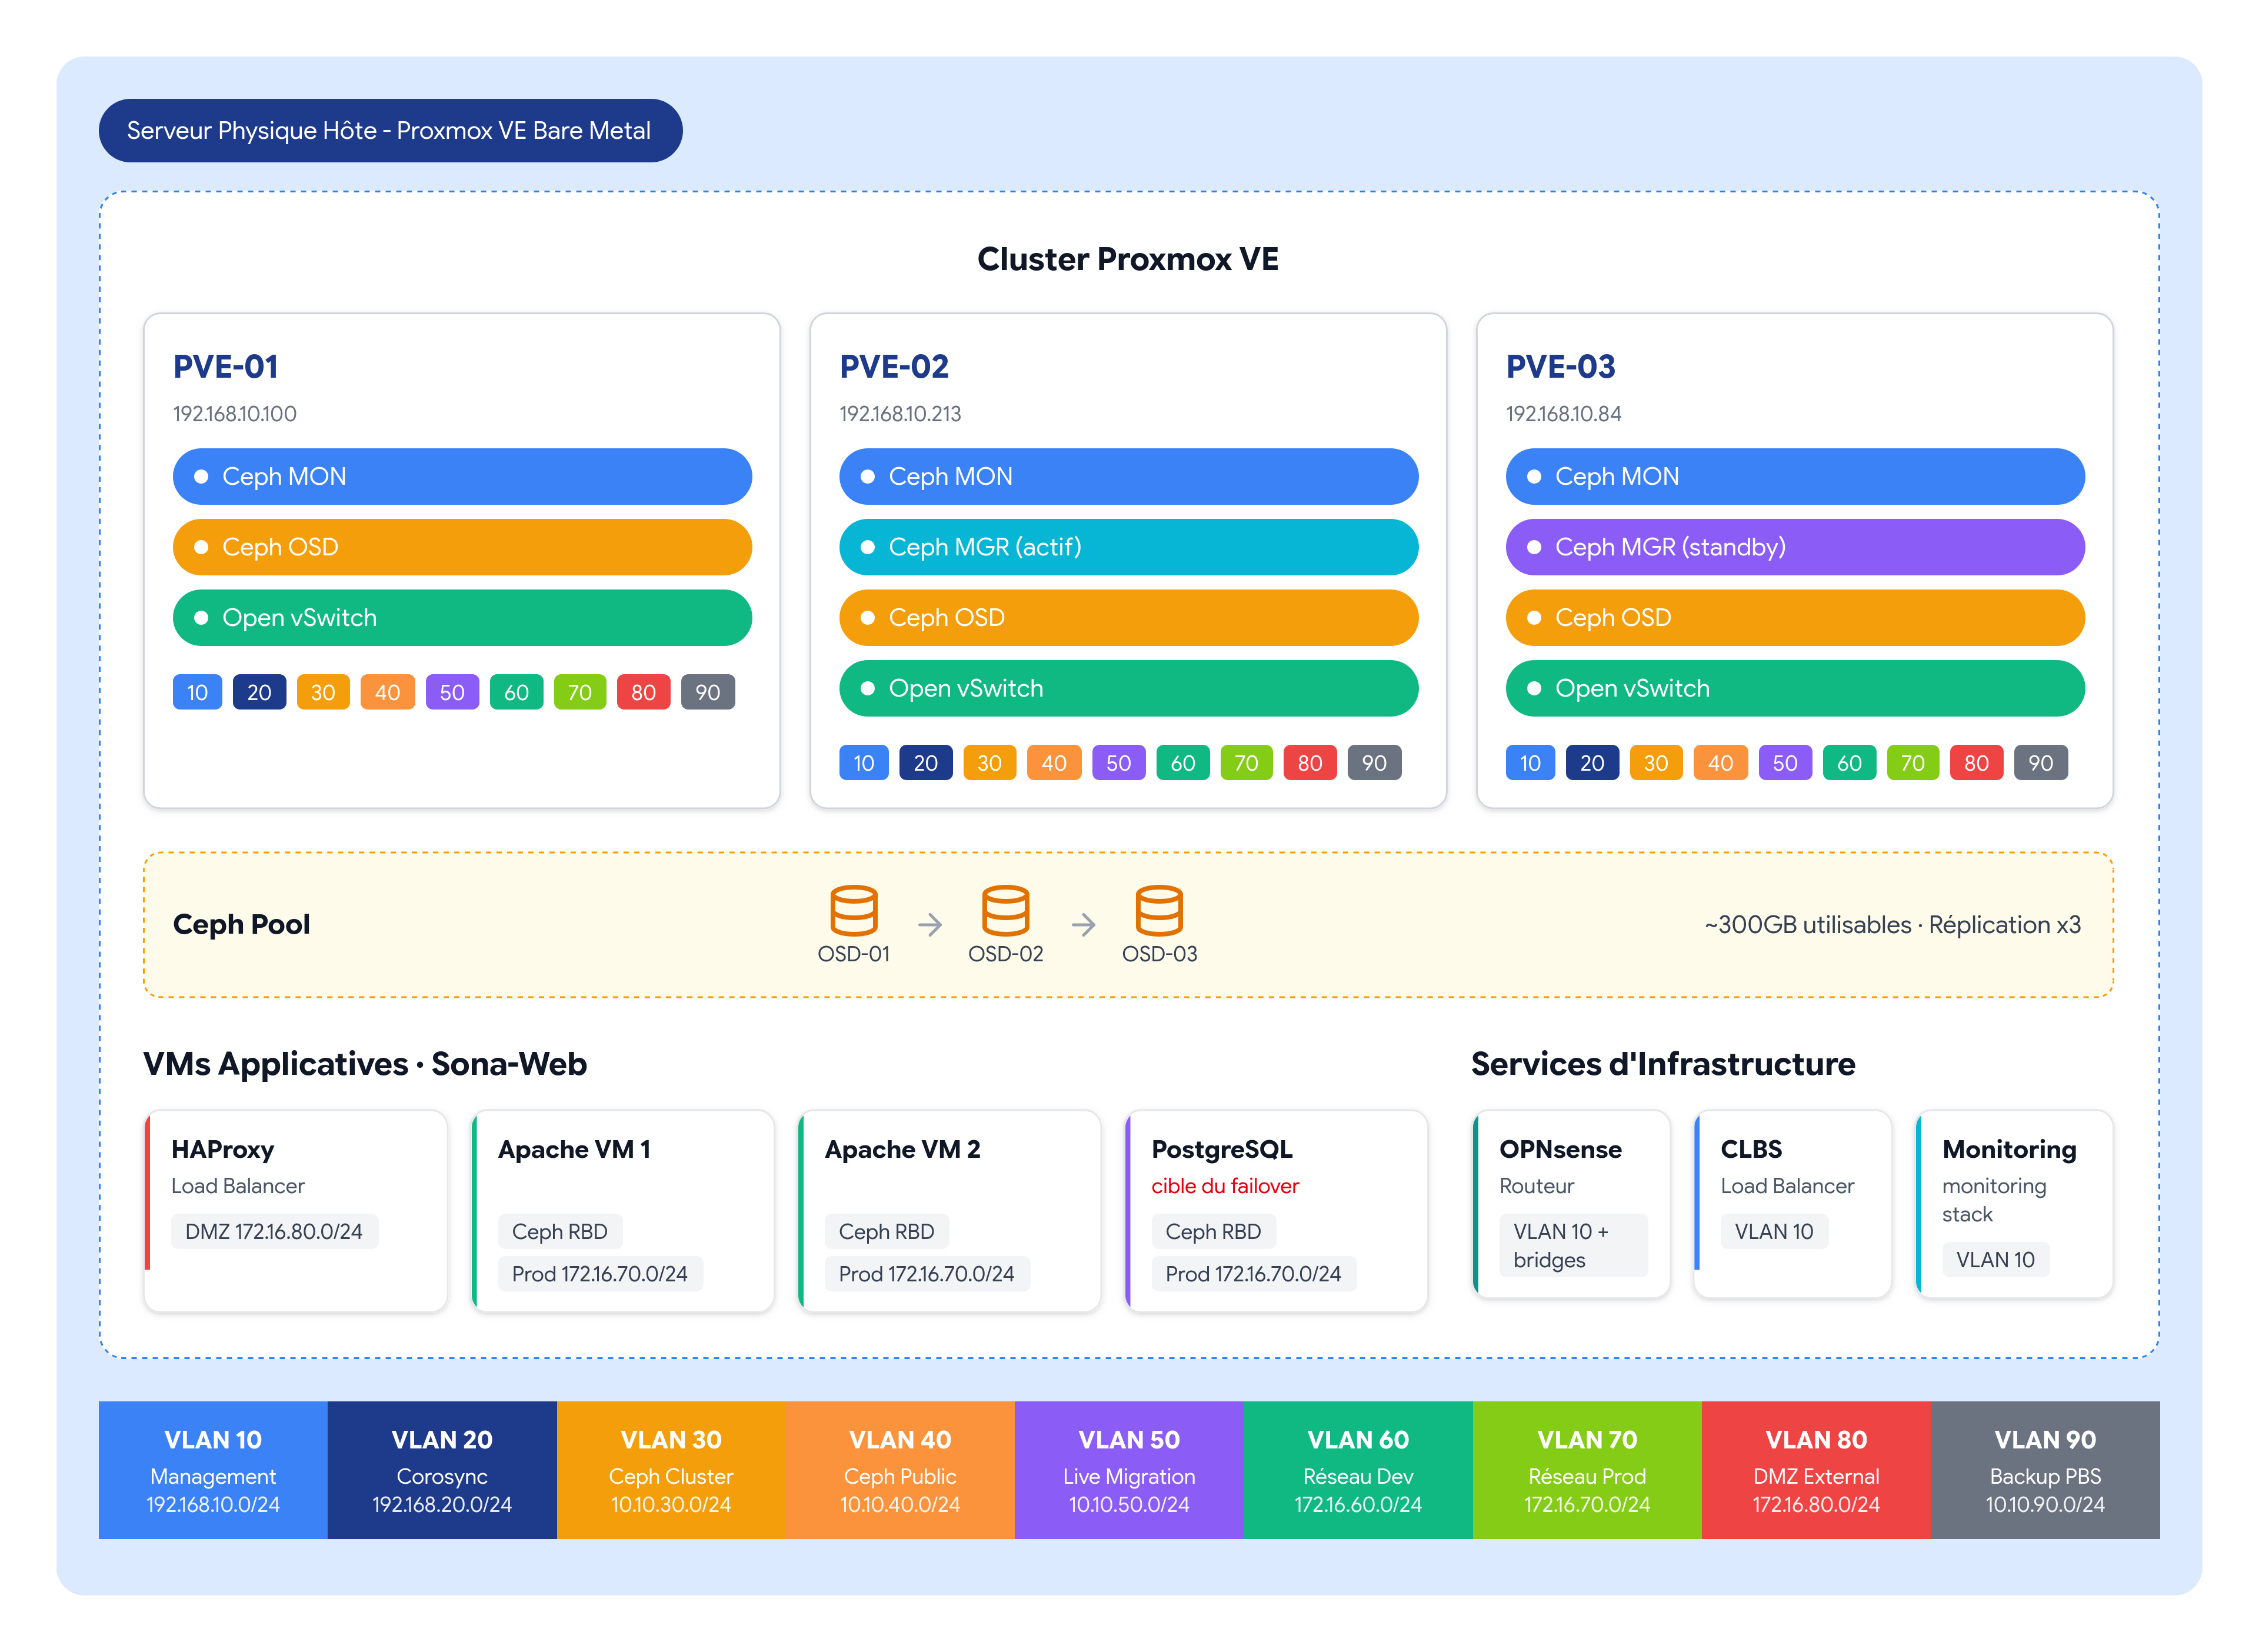
\includegraphics[width=0.9\textwidth]{image/ch3/architecture-hci.jpg}
        \caption{Architecture Globale de l'Infrastructure}
        \label{fig:arch-globale}
    \end{center}
\end{figure}


% %%%%%%%%%%%%%%%%%%%%%%%%%%%%%%%%%%%%%%%%%%%%%%%%%%%%%%%%%%%%
% PARTIE 1 : COMPUTE
% %%%%%%%%%%%%%%%%%%%%%%%%%%%%%%%%%%%%%%%%%%%%%%%%%%%%%%%%%%%%

{\color{bleu} \section{Partie I : Compute}}

% ============================================================
{\color{bleu} \section{Architecture Physique}}
% ============================================================

{\color{bleuu} \subsection{Infrastructure Physique}}

\par L'infrastructure physique est constituée de trois serveurs Dell PowerEdge R720 mis à disposition par le Centre d'innovation de Sonatrach. Ces serveurs constitueront les trois n\oe{}uds physiques du cluster Proxmox : PVE-01, PVE-02 et PVE-03. Proxmox VE sera installé directement en mode bare metal sur chacun d'eux, sans couche de virtualisation intermédiaire.\\

\par Le Dell PowerEdge R720 est un serveur rack 2U de la gamme Enterprise de Dell, reconnu pour sa robustesse et sa capacité d'extension. Il est équipé de processeurs Intel Xeon E5-2600 et supporte jusqu'à 768 GB de RAM, ce qui en fait une plateforme adaptée aux charges de virtualisation intensive et au stockage distribué. Dans notre déploiement, chaque serveur sera configuré avec 64 GB de RAM et deux disques SAS répartis selon les rôles définis ci-dessous.\\

\par \textbf{Allocation des disques par n\oe{}ud}\\

\par Chaque serveur disposera de deux disques SAS répartis en deux catégories fonctionnelles, conformément aux recommandations Proxmox et Ceph concernant la séparation des I/O système et stockage :\\

\begin{itemize}
    \item \textbf{Disque système (sda -- 1 x 300 GB SAS) :} dédié au système d'exploitation Proxmox VE. Cette séparation garantit que les opérations de réplication Ceph ne concurrencent pas les I/O système du n\oe{}ud, conformément aux recommandations officielles Proxmox [10].
    \item \textbf{Disque OSD Ceph (sdb -- 1 x 300 GB SAS) :} affecté à un OSD Ceph distinct, contribuant au stockage distribué du cluster. Chaque n\oe{}ud apportera ainsi 1 OSD au pool global.
\end{itemize}

\begin{center}
\begin{tabular}{|p{3cm}|p{3cm}|p{3cm}|p{4cm}|}
\hline
\textbf{Composant} & \textbf{Valeur par n\oe{}ud} & \textbf{Total cluster} & \textbf{Justification} \\
\hline
\textbf{Modèle serveur} & Dell PowerEdge R720 & 3 serveurs & Fourni par Sonatrach \\
\hline
\textbf{RAM} & 64 GB & 192 GB & Proxmox + Ceph + VMs [10][14] \\
\hline
\textbf{Disque OS (sda)} & 1 x 300 GB SAS & 3 x 300 GB & Isolation I/O hôte / Ceph [10] \\
\hline
\textbf{Disque OSD (sdb)} & 1 x 300 GB SAS & 3 x 300 GB & 1 OSD par n\oe{}ud [12][13] \\
\hline
\textbf{IP Management} & Voir tableau 3-4 & & VxLAN 10 -- réseau Sonatrach \\
\hline
\end{tabular}
\end{center}
\noindent \textit{Tableau 3-1 : Dimensionnement physique des serveurs Dell PowerEdge R720}\\

% ============================================================
{\color{bleu} \section{Architecture du Cluster Proxmox}}
% ============================================================

{\color{bleuu} \subsection{Organisation du Cluster}}

\par Le cluster Proxmox sera constitué de trois n\oe{}uds physiques identiques interconnectés via le réseau de Sonatrach. Chaque n\oe{}ud exécutera Proxmox VE en bare metal sur un serveur Dell PowerEdge R720 dédié. Le trafic Corosync sera transporté sur un réseau logique dédié (VxLAN ID 20) afin de garantir la stabilité du quorum indépendamment des autres flux réseau.\\

\par Cette organisation à trois n\oe{}uds physiques est le minimum requis par Proxmox pour garantir un quorum stable et éviter les situations de split-brain [21]. La défaillance complète d'un n\oe{}ud physique sera absorbée par le mécanisme HA de Proxmox, les deux n\oe{}uds survivants maintenant le quorum (2/3) et continuant à opérer normalement.\\

\begin{center}
\begin{tabular}{|p{4cm}|p{4cm}|p{5cm}|}
\hline
\textbf{N\oe{}ud} & \textbf{Nom d'hôte} & \textbf{Adresse IP Management (192.168.10.0/24)} \\
\hline
N\oe{}ud 1 & PVE-01 & 192.168.10.100 \\
\hline
N\oe{}ud 2 & PVE-02 & 192.168.10.213 \\
\hline
N\oe{}ud 3 & PVE-03 & 192.168.10.84 \\
\hline
\end{tabular}
\end{center}
\noindent \textit{Tableau 3-2 : Adresses IP de management des n\oe{}uds Proxmox physiques}\\

{\color{bleuu} \subsection{Mécanisme de Quorum et Corosync}}

\par Corosync est le framework de communication de cluster utilisé par Proxmox pour assurer le consensus entre les n\oe{}uds. Il enverra des messages de heartbeat entre les n\oe{}uds à intervalles réguliers via le réseau logique VxLAN ID 20 dédié. Lorsqu'un n\oe{}ud cessera de répondre, Corosync déclenchera une procédure de vote pour déterminer si le cluster dispose encore du quorum nécessaire pour continuer à opérer [20].\\

\par Le quorum dans un cluster de trois n\oe{}uds est atteint dès que deux n\oe{}uds sur trois sont opérationnels. La perte de deux n\oe{}uds simultanément entraînerait la perte du quorum et le gel du cluster pour éviter toute corruption des données, comportement conforme aux recommandations de sécurité Proxmox [6].\\

{\color{bleuu} \subsection{Haute Disponibilité}}

\par Le mécanisme de haute disponibilité (HA) de Proxmox s'appuiera sur Corosync pour la détection des pannes et sur le Resource Manager HA pour les décisions de basculement [6]. Lorsqu'un n\oe{}ud sera déclaré défaillant, le HA Manager identifiera les VMs qui y résidaient et déclenchera leur redémarrage automatique sur un des n\oe{}uds survivants.\\

\par Ce mécanisme est rendu possible par le stockage partagé Ceph : les disques des VMs étant stockés sur le pool Ceph commun et accessibles depuis n'importe quel n\oe{}ud du cluster, le redémarrage d'une VM sur un n\oe{}ud différent ne nécessitera aucun transfert de données. La VM redémarrera directement depuis le volume Ceph RBD existant, ce qui minimise le temps de récupération après panne (RTO). Selon la documentation Proxmox, ce délai de basculement est typiquement compris entre 60 et 120 secondes.\\

\par Dans notre architecture, toutes les VMs de l'application Sona-Web seront configurées en mode HA, avec une priorité de basculement définie pour garantir que le load balancer HAProxy est redémarré en premier, suivi des serveurs web, puis de la base de données PostgreSQL.\\

{\color{bleuu} \subsection{Matrice des Scénarios de Défaillance}}

\par Le tableau suivant recense les scénarios de défaillance envisagés 
et le comportement attendu du système dans chacun d'eux :\\

\begin{center}
\begin{tabular}{|p{2.8cm}|p{2.5cm}|p{7cm}|p{2cm}|}
\hline
\textbf{Scénario} & \textbf{Composant affecté} & \textbf{Comportement du système} & \textbf{RTO estimé} \\
\hline
Panne d'un n\oe{}ud physique & PVE-01, PVE-02 ou PVE-03 &
Corosync détecte la perte de heartbeat. Le HA Manager redémarre les
VMs HA sur les n\oe{}uds survivants (quorum 2/3 maintenu). Ceph passe
en état \texttt{degraded} mais reste accessible (\texttt{min\_size=2}).
& 60--120 s \\
\hline
Panne d'un OSD Ceph & Disque \texttt{sdb} sur un n\oe{}ud &
Ceph marque l'OSD \texttt{down} puis \texttt{out}. Le pool passe en
état \texttt{degraded} (2 répliques sur 3) mais les I/O continuent.
Dès rétablissement, un \textit{backfill} automatique reconstitue la
troisième réplique.
& Aucune coupure \\
\hline
Panne du MGR actif & PVE-02 (MGR actif) &
Le MGR en standby (PVE-03) prend le relais automatiquement.
L'endpoint Prometheus (port 9283) reste disponible sans intervention
manuelle.
& \textless{} 30 s \\
\hline
Panne de deux n\oe{}uds simultanés & Deux des trois n\oe{}uds &
Perte du quorum Corosync et Ceph. Le n\oe{}ud survivant se gèle pour
prévenir tout split-brain. Le cluster devient inaccessible et une
intervention manuelle est requise.
& N/A \\
\hline
Panne de la VM OPNsense & VM routeur/pare-feu &
Proxmox HA redémarre la VM sur un n\oe{}ud survivant. Le trafic
inter-réseaux est interrompu pendant la durée du redémarrage, ce qui
constitue la limite connue de cette approche par rapport à un
basculement CARP sans interruption.
& 60--120 s \\
\hline
Partition réseau (split-brain) & Réseau VxLAN 20 (Corosync) &
Le groupe minoritaire (1 n\oe{}ud) perd le quorum et se gèle. Le
groupe majoritaire (2 n\oe{}uds) continue d'opérer. Le gel prévient
toute écriture divergente sur Ceph.
& Aucune coupure côté majoritaire \\
\hline
Défaillance du service CLBS & VM CLBS &
Aucun impact applicatif. Le service redémarre automatiquement
(\texttt{Restart=always} dans l'unit systemd). Si la VM elle-même
est défaillante, Proxmox HA la redémarre sur un autre n\oe{}ud.
& Aucune coupure applicative \\
\hline
\end{tabular}
\end{center}
\noindent \textit{Tableau 3-X : Matrice des scénarios de défaillance et comportements attendus}\\ee

% ============================================================
{\color{bleu} \section{Mécanisme d'Équilibrage Dynamique : CLBS}}
% ============================================================

{\color{bleuu} \subsection{Contexte et Besoin}}

\par Proxmox VE intègre nativement un mécanisme de haute disponibilité réactif : lorsqu'un n\oe{}ud tombe en panne, les VMs qui y résidaient sont automatiquement redémarrées sur les n\oe{}uds survivants. Cependant, Proxmox ne dispose d'aucun mécanisme proactif d'équilibrage de charge, contrairement à VMware vSphere qui propose le DRS (Distributed Resource Scheduler) [18].\\

\par Sans équilibrage proactif, un cluster Proxmox peut se retrouver dans une situation où un n\oe{}ud est saturé à 90\% de CPU tandis qu'un autre n\oe{}ud reste à 20\% d'utilisation. Proxmox n'intervient pas dans ce cas, laissant le déséquilibre persister et dégradant les performances des VMs sur le n\oe{}ud surchargé. Ce déséquilibre représente un gaspillage significatif de ressources et une dégradation de la qualité de service [18].\\

{\color{bleuu} \subsection{Base Algorithmique : CSLB}}

\par Notre mécanisme, que nous nommons \textbf{CLBS (Central Load Balancing Scheduler)}, est une adaptation du CSLB (Central Scheduler Load Balancing) [17]. L'algorithme CSLB original repose sur cinq phases : évaluation de charge, détermination de rentabilité, calcul du vecteur de transfert, sélection de VM et exécution de la migration.\\

\par Dans CSLB, la charge CPU de chaque n\oe{}ud est évaluée par rapport à un seuil dynamique (moyenne des charges de tous les n\oe{}uds). Une bande modérée est calculée autour de ce seuil selon la formule :

\begin{center}
$\text{seuil} = \frac{\sum_{i=1}^{n} \alpha_i}{n}$, \quad
$\text{diff} = |\text{seuil} - \frac{\alpha_{min} + \alpha_{max}}{2}|$ \\
$\alpha_i $: le CPU du nœud i \\
$n :$ Nombre du nœuds
\end{center}

\par La bande modérée est définie à $\pm \max(\text{diff}, 10\%)$ autour du seuil. Les n\oe{}uds hors bande modérée sont candidats à une action d'équilibrage.\\

{\color{bleuu} \subsection{Modifications Apportées au CSLB}}

\par Notre adaptation du CSLB intègre plusieurs modifications
significatives par rapport à l'algorithme original. Le service est
implémenté en \textbf{Go} (Golang), retenu pour sa faible empreinte
mémoire, sa gestion native de la concurrence via les goroutines, et
la simplicité de son déploiement sous forme de binaire statique dans
un service systemd.\\

\par \textbf{Extension à la RAM.} Le CSLB original ne considère que
le CPU. Notre implémentation étend l'évaluation à la RAM, calculant
une bande modérée indépendante pour chaque métrique. Un n\oe{}ud est
considéré surchargé si l'une ou l'autre dépasse sa bande respective.\\

\par \textbf{Seuil minimum de migration.} Une migration n'est
déclenchée que si la charge du n\oe{}ud surchargé dépasse un seuil
absolu de 50\% (CPU ou RAM). En dessous, même si le n\oe{}ud est
statistiquement hors de sa bande, la migration est jugée non rentable,
évitant des déplacements inutiles dans un cluster globalement
sous-chargé.\\

\par \textbf{Sélection du n\oe{}ud destination pondérée avec
vérification préalable.} Le choix du n\oe{}ud destination se fonde
sur un score de différentiel pondéré :

\begin{center}
$\text{score} = \Delta_{CPU} \times 0.7 + \Delta_{RAM} \times 0.3$
\end{center}

\par Avant de valider la destination, CLBS simule l'état post-migration
du n\oe{}ud cible en y ajoutant la consommation de la VM candidate.
Si le résultat dépasse la bande haute, ce n\oe{}ud est écarté et le
candidat suivant est évalué, évitant de transférer la surcharge d'un
n\oe{}ud à l'autre.\\

\par \textbf{Exclusion des VMs système.} OPNsense, la VM de monitoring
et la VM CLBS elle-même sont explicitement exclues du périmètre de
migration : migrer l'une d'elles interromprait respectivement le
routage inter-réseaux, les métriques nécessaires aux décisions CLBS,
ou le service lui-même.\\

\par \textbf{Cadence et unicité de migration par cycle.} CLBS
s'exécute toutes les 60 secondes et ne peut déclencher qu'une seule
migration par cycle. Cette contrainte laisse au cluster le temps
d'intégrer le changement de charge, prévient les effets de cascade,
et exclut explicitement la VM migrée du cycle suivant.\\

\par \textbf{Cooldown post-migration.} Après chaque migration réussie,
une période de repos de \textbf{5 minutes} est appliquée, garantissant
que les métriques InfluxDB, lissées sur une fenêtre glissante de
5 minutes, ont intégré l'impact de la migration avant toute nouvelle
décision.\\

\par \textbf{Mécanisme anti-oscillation et disjoncteurs.} Plusieurs
niveaux de protection contre les comportements instables sont mis
en place :

\begin{itemize}
    \item \textbf{VM migration pause (30 minutes) :} si une même VM est
    migrée deux fois en moins de 10 minutes, la VM est gelée pendant
    \textbf{30 minutes} et l'administrateur est notifié via
    l'Alertmanager Grafana.

    \item \textbf{Migration Storm :} si CLBS enregistre 6 migrations
    ou plus en 30 minutes, il s'arrête automatiquement pendant une
    heure et envoie une alerte d'urgence. Ce disjoncteur
    (\textit{circuit breaker}) préserve la stabilité du cluster en
    cas de dérive algorithmique ou de charge pathologique.
\end{itemize}

\par \textbf{Système de notification.} Les alertes sont acheminées
via l'Alertmanager intégré à notre tableau de bord Grafana, qui
expose déjà les métriques CLBS en temps réel (historique des
migrations, état des cooldowns, score de charge par n\oe{}ud). Des
webhooks sortants pourront être configurés pour intégrer ces
notifications à d'autres canaux selon les préférences opérationnelles.\\

\par \textbf{Collecte des métriques.} CLBS combine deux sources :
l'API REST Proxmox pour les métriques courantes des n\oe{}uds, et
InfluxDB via le client Go officiel pour les moyennes glissantes sur
5 minutes de consommation CPU des VMs, insuffisamment exposées par
l'API Proxmox. Cette combinaison garantit des décisions fondées sur
des données lissées plutôt que sur des pics instantanés.\\

\par \textbf{Authentification dédiée.} CLBS utilise une clé API
Proxmox dédiée avec les permissions minimales nécessaires (lecture
des métriques, déclenchement de migrations), conformément au principe
du moindre privilège.\\

\begin{figure}[H]
    \begin{center}
        % Organigramme de décision du service CLBS (réduit pour laisser apparaître le titre)
\scalebox{0.8}{%
\begin{tikzpicture}[
  node distance=0.8cm and 1.5cm,
  box/.style={rectangle, rounded corners, draw=black, fill=blue!10,
               text width=5cm, align=center, minimum height=0.8cm, font=\small},
  decision/.style={diamond, draw=black, fill=orange!20, aspect=2,
                   text width=3cm, align=center, font=\small},
  arrow/.style={-{Latex}, thick},
  ]

  \node[box] (start) {Début du cycle (60s)};
  \node[box, below=of start] (fetch) {Récupérer métriques CPU \& RAM\\(moyenne 5 min) depuis InfluxDB};
  \node[box, below=of fetch] (calc) {Calculer seuil et bande modérée\\pour CPU et RAM};
  \node[decision, below=of calc] (heavy) {N\oe{}ud surchargé\\(hors bande haute)\\ ET charge $> 50\%$ ?};
  \node[box, right=2cm of heavy] (wait) {Attendre prochain\\cycle};
  \node[box, below=of heavy] (vmsel) {Sélectionner VM candidate\\(CSLB vecteur de transfert,\\cooldown respecté)};
  \node[box, below=of vmsel] (destsel) {Calculer score destination :\\$\Delta_{CPU} \times 0.7 + \Delta_{RAM} \times 0.3$};
  \node[decision, below=of destsel] (found) {N\oe{}ud destination\\trouvé ?};
  \node[box, right=2cm of found] (nocand) {Aucune action,\\attendre prochain cycle};
  \node[box, below=of found] (migrate) {Déclencher live migration\\via API Proxmox (VxLAN 50)};
  \node[box, below=of migrate] (log) {Enregistrer dans InfluxDB\\Appliquer cooldown (10 min)};
  \node[box, below=of log] (end) {Fin du cycle};

  \draw[arrow] (start) -- (fetch);
  \draw[arrow] (fetch) -- (calc);
  \draw[arrow] (calc) -- (heavy);
  \draw[arrow] (heavy) -- node[above]{\small Non} (wait);
  \draw[arrow] (heavy) -- node[right]{\small Oui} (vmsel);
  \draw[arrow] (vmsel) -- (destsel);
  \draw[arrow] (destsel) -- (found);
  \draw[arrow] (found) -- node[above]{\small Non} (nocand);
  \draw[arrow] (found) -- node[right]{\small Oui} (migrate);
  \draw[arrow] (migrate) -- (log);
  \draw[arrow] (log) -- (end);
\end{tikzpicture}%
}

        \caption{Logique de Décision du Mécanisme CLBS}
        \label{fig:clbs}
    \end{center}
\end{figure}

{\color{bleuu} \subsection{Algorithme de Décision (Pseudocode)}}

\begin{verbatim}
toutes les 60 secondes :
  récupérer métriques CPU et RAM moyennées (5 min) depuis InfluxDB
  calculer seuil_cpu, bande_moderee_cpu
  calculer seuil_ram, bande_moderee_ram

  pour chaque noeud N :
    si (cpu_N > bande_haute_cpu OU ram_N > bande_haute_ram)
       ET (cpu_N > 50% OU ram_N > 50%) :

      candidats_vm = VMs sur N non migrées récemment (cooldown 10 min)
      vm_cible = VM dont la charge est la plus proche du
                 vecteur de transfert calculé (phase 3 CSLB)

      pour chaque noeud destination D (band légère) :
        score_D = (cpu_N - cpu_D) * 0.7 + (ram_N - ram_D) * 0.3
      noeud_dest = D avec score_D maximal

      si noeud_dest trouvé :
        déclencher live migration vm_cible vers noeud_dest
          via API Proxmox (VxLAN 50)
        enregistrer migration dans InfluxDB
        appliquer cooldown anti-oscillation (10 min sur vm_cible)
\end{verbatim}

% ============================================================
{\color{bleu} \section{Application de Démonstration : Sona-Web}}
% ============================================================

{\color{bleuu} \subsection{Architecture Applicative}}

\par Sona-Web est une application web déployée sur le cluster pour démontrer
les capacités de haute disponibilité et de live migration de l'infrastructure.
Elle est constituée de quatre VMs Debian~12 interconnectées dans le réseau
192.168.10.0/24 :

\begin{itemize}
    \item \textbf{HAProxy (VM-201)~:} point d'entrée unique de l'application,
    accessible à l'adresse 192.168.10.111 sur le port 8080. Il distribue les requêtes HTTP
    entrantes entre les deux serveurs applicatifs selon l'algorithme
    round-robin et surveille leur disponibilité toutes les 200~ms via un
    health check \texttt{GET /health}, basculant en moins de 200~ms vers
    l'instance disponible en cas d'indisponibilité (\texttt{fall 1}).

    \item \textbf{Flask app-1 (VM-202) et app-2 (VM-203)~:} deux instances
    identiques de l'application Python Flask, servies respectivement aux
    adresses 192.168.10.112 et 192.168.10.114 sur le port 8000. Chaque
    instance enregistre de manière asynchrone en base de données toutes les
    requêtes reçues, ce qui permet de reconstituer l'historique complet
    après une migration et de constater qu'aucune requête n'a été perdue.

    \item \textbf{PostgreSQL (VM-204)~:} serveur de base de données centralisé
    à l'adresse 192.168.10.115 sur le port 5432, dont le disque est stocké sur un volume
    CEPH~RBD. Il centralise les enregistrements des deux instances Flask,
    garantissant un historique cohérent quel que soit le nœud hébergeant
    les VMs applicatives.
\end{itemize}

Les quatre VMs sont toutes membres du groupe HA \texttt{sona-group} et leurs
disques résident sur le pool CEPH~RBD partagé entre les trois nœuds Proxmox,
condition nécessaire à la live migration à chaud. Les adresses IP sont
configurées de manière statique dans \texttt{/etc/network/interfaces} afin
de garantir leur stabilité après migration, sans dépendance à un serveur DHCP.

\begin{figure}[H]
    \begin{center}
        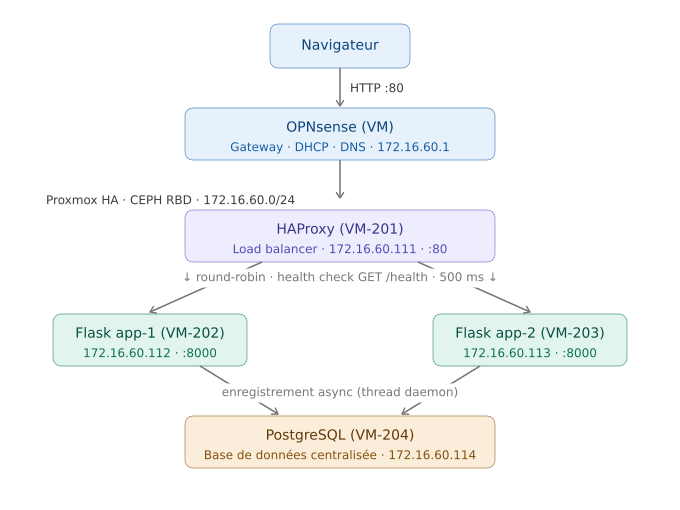
\includegraphics[width=0.85\textwidth]{image/ch3/architecture_sona_web (2).png}
        \caption{Architecture Applicative Sona-Web}
        \label{fig:sona-web}
    \end{center}
\end{figure}

{\color{bleuu} \subsection{Scénario de Validation HA}}

\par Le scénario de démonstration se déroule en quatre temps~: affichage de
l'alternance round-robin entre app-1 et app-2 (validation de l'équilibrage
de charge), puis déclenchement d'une live migration de VM-202 (\texttt{app-1})
vers un autre nœud via la commande \texttt{qm migrate 202 pve-node-2 --online}.

Pendant la migration, Proxmox transfère l'état mémoire de la VM sans arrêter
son exécution~; lorsque la synchronisation atteint \textasciitilde{}99\,\%, la
VM est suspendue quelques dizaines de millisecondes le temps de transférer
le delta final, puis reprend sur le nœud cible. HAProxy détecte l'indisponibilité
transitoire en 200~ms maximum (\texttt{fall 1}) et redirige automatiquement
l'intégralité du trafic vers app-2. Une fois la migration terminée, app-1 est
remise en service dès le premier health check réussi (\texttt{rise 1}).

L'analyse post-migration de la base PostgreSQL confirme qu'aucune requête
n'a été perdue. Le schéma de la table \texttt{requests} comprend les champs
suivants : \texttt{id} (clé primaire), \texttt{instance\_id}, \texttt{path},
\texttt{request\_time} (horodatage automatique), \texttt{client\_ip} et
\texttt{user\_agent}. La requête ci-dessous permet de vérifier la répartition
des requêtes entre les deux instances sur la dernière heure~:

\begin{lstlisting}[language=SQL]
SELECT instance_id,
       COUNT(*) AS total
FROM requests
WHERE request_time > NOW() - INTERVAL '1 hour'
GROUP BY instance_id;
\end{lstlisting}

Ce résultat valide le fonctionnement de la haute disponibilité~: zéro coupure
observable pour l'utilisateur lors d'une migration live sur le cluster Proxmox.

% ============================================================
{\color{bleu} \section{Automatisation}}
% ============================================================

{\color{bleuu} \subsection{Ansible : Périmètre et Playbooks}}

\par Ansible sera utilisé comme outil d'automatisation principal pour trois domaines distincts, chacun correspondant à un playbook dédié.\\

\par \textbf{Playbook 1 : intégration d'un nouveau n\oe{}ud au cluster.} Ce playbook automatisera l'ensemble de la procédure d'intégration d'un serveur fraîchement installé (via PXE) dans le cluster Proxmox existant. Il couvrira la configuration réseau (création des ports VxLAN OVS, assignation des adresses IP sur chaque réseau logique), le peuplement du cluster Corosync, l'initialisation et l'ajout de l'OSD Ceph du nouveau n\oe{}ud, et la configuration des exports de métriques vers InfluxDB.\\

\par \textbf{Playbook 2 : provisionnement de VMs et de conteneurs.} Ce playbook automatisera la création de VMs et de conteneurs LXC à partir de templates cloud-init stockés dans le pool Ceph. Il intégrera la configuration réseau automatique via DHCP (OPNsense dnsmasq), l'assignation au bon bridge OVS (Dev, Prod ou DMZ) selon le paramètre passé, et la configuration initiale du système (mise à jour des paquets, création des comptes Ansible).\\

\par \textbf{Playbook 3 : migration Dev vers Prod ou DMZ.} Ce playbook gérera la promotion d'une VM ou d'un ensemble de VMs de l'environnement de développement vers la production ou la DMZ. Pour les applications microservices, il assurera la reconfiguration réseau de chaque composant, la mise à jour des règles de pare-feu OPNsense correspondantes, et la vérification de la connectivité post-migration.\\

\par Ansible sera exécuté depuis les postes de travail des développeurs via des comptes dédiés sur les n\oe{}uds Proxmox, en utilisant l'accès SSH sur le réseau de management 192.168.10.0/24.\\

{\color{bleuu} \subsection{PXE et TFTP : Provisionnement Automatisé des N\oe{}uds}}

\par Dans une optique de scalabilité horizontale, un pipeline de provisionnement
en deux phases a été mis en place pour automatiser l'intégration de tout nouveau
serveur physique au cluster Proxmox VE, sans aucune intervention manuelle.

\par \textbf{Infrastructure de provisionnement.} Le serveur \textbf{OPNsense}
(adresse \texttt{192.168.10.65}), déjà en charge des services DHCP, DNS et
gateway internet de l'infrastructure, est configuré avec les options DHCP
\texttt{66} (\textit{Next Server}) et \texttt{67} (\textit{Bootfile Name})
pointant vers un conteneur LXC dédié. Ce conteneur héberge le serveur TFTP
ainsi qu'un serveur HTTP Nginx pour la distribution des fichiers d'installation.
Cette architecture évite toute redondance de services DHCP et s'appuie
intégralement sur l'infrastructure réseau existante.

\par \textbf{Phase 1 -- Installation automatique via PXE.} Le protocole
\textbf{PXE} (\textit{Preboot eXecution Environment}) est un standard Intel
gravé dans le firmware des cartes réseau, permettant à une machine de démarrer
depuis le réseau avant toute installation d'un système d'exploitation.
Lorsqu'un nouveau serveur physique est mis sous tension, la séquence suivante
s'exécute automatiquement :

\begin{enumerate}
    \item Le serveur envoie une requête \textbf{DHCP} ; OPNsense lui attribue
    une adresse IP temporaire et lui indique l'adresse du serveur de boot ainsi
    que le fichier bootloader à récupérer ;

    \item Le firmware PXE contacte le serveur \textbf{TFTP}
    (\textit{Trivial File Transfer Protocol}, UDP/69) pour télécharger
    \textit{uniquement} le bootloader (\texttt{pxelinux.0}) et le kernel Linux
    d'amorçage. Le protocole TFTP est retenu à cette étape car il est le seul
    protocole implémentable dans un firmware de quelques dizaines de kilo-octets,
    sans nécessiter de système d'exploitation préalable. Les protocoles FTP, SFTP
    ou SSH sont inutilisables à ce stade, car ils requièrent un OS et des
    bibliothèques logicielles qui n'existent pas encore ;

    \item Une fois le kernel démarré en mémoire vive, l'image d'installation
    Proxmox VE (\textasciitilde{}800 Mo) est téléchargée via \textbf{HTTP} depuis
    le serveur Nginx du conteneur LXC dédié. Ce choix est délibéré : TFTP,
    reposant sur UDP sans mécanisme de reprise sur erreur ni contrôle de flux,
    est inadapté au transfert de fichiers volumineux ; HTTP (TCP) garantit
    l'intégrité et la performance du transfert ;

    \item L'installateur Proxmox lit un fichier de réponses
    (\textit{Answer File} / \texttt{preseed.cfg}), hébergé sur le même serveur
    HTTP, contenant les paramètres d'installation : partitionnement du disque,
    nom d'hôte, fuseau horaire (\texttt{Africa/Algiers}) et langue.
    L'installation s'effectue sans aucune frappe clavier ;

    \item Le serveur redémarre automatiquement sur Proxmox VE
    fraîchement installé.
\end{enumerate}

\par \textbf{Phase 2 -- Intégration au cluster via Ansible.} A l'issue du
redémarrage, le nouveau n\oe{}ud dispose d'un Proxmox VE fonctionnel mais
isolé. Un \textbf{Playbook Ansible} prend alors le relais via SSH pour réaliser
l'intégration complète au cluster existant :

\begin{itemize}
    \item Adhésion au cluster \textbf{Corosync} pour la haute disponibilité ;
    \item Configuration des interfaces \textbf{Open vSwitch} et des tunnels
    \textbf{VxLAN} inter-n\oe{}uds ;
    \item Intégration des disques physiques comme \textbf{OSDs} dans le cluster
    de stockage distribué \textbf{CEPH} ;
    \item Rattachement au groupe \textbf{HA Proxmox}
    (\texttt{sona-ha-group}) ;
    \item Déclaration du n\oe{}ud comme nouvelle cible dans
    \textbf{Prometheus} pour le monitoring existant.
\end{itemize}

\par Ce découpage en deux phases répond à une contrainte technique fondamentale :
PXE et TFTP interviennent dans un environnement \textit{pre-OS} où aucun client
SSH ne peut fonctionner, tandis qu'Ansible nécessite un système d'exploitation
opérationnel et une connectivité SSH, conditions remplies uniquement à l'issue
de la Phase 1. L'ensemble du pipeline permet l'ajout d'un nouveau n\oe{}ud au
cluster en moins de 25 minutes, sans intervention manuelle, répondant ainsi
à l'exigence de scalabilité horizontale du projet.

% ============================================================
{\color{bleu} \section{Architecture du Monitoring}}
% ============================================================

\par La stack de monitoring sera déployée sur une VM dédiée accessible depuis le réseau de management à l'adresse 192.168.10.99. Elle comprendra trois composants complémentaires, chacun couvrant un périmètre de métriques distinct.\\

\par \textbf{Proxmox Metrics Server et InfluxDB.} Proxmox VE supporte nativement l'export de ses métriques générales (CPU, RAM, réseau et stockage des n\oe{}uds et des VMs) vers une base de données InfluxDB via son interface de configuration [15]. Chaque n\oe{}ud poussera automatiquement ses métriques à intervalles réguliers sans nécessiter d'agent supplémentaire. InfluxDB stockera ainsi l'historique complet des métriques d'infrastructure, utilisé à la fois par Grafana pour la visualisation et par le service CLBS pour ses décisions de migration.\\

\par \textbf{Prometheus et Ceph MGR.} Les métriques détaillées du cluster Ceph (état des OSDs, latence des I/O, utilisation du pool, santé du cluster) ne sont pas disponibles via le Proxmox Metrics Server. Le n\oe{}ud MGR actif de Ceph expose nativement un endpoint Prometheus sur le port 9283. Prometheus sera configuré pour scraper cet endpoint, fournissant ainsi une visibilité complète sur la santé du stockage distribué.\\

\par \textbf{Grafana.} Grafana sera connecté à la fois à InfluxDB et à Prometheus comme sources de données, permettant de construire des tableaux de bord unifiés couvrant l'ensemble de l'infrastructure : utilisation des ressources par n\oe{}ud, état du cluster Ceph, historique des migrations CLBS, et alertes de surcharge.\\


% %%%%%%%%%%%%%%%%%%%%%%%%%%%%%%%%%%%%%%%%%%%%%%%%%%%%%%%%%%%%
% PARTIE 2 : STORAGE
% %%%%%%%%%%%%%%%%%%%%%%%%%%%%%%%%%%%%%%%%%%%%%%%%%%%%%%%%%%%%

{\color{bleu} \section{Partie II : Storage}}

% ============================================================
{\color{bleu} \section{Architecture du Stockage Ceph}}
% ============================================================

{\color{bleuu} \subsection{Composants du Cluster Ceph}}

\par Le cluster Ceph sera composé des services suivants, répartis sur les trois n\oe{}uds physiques :

\begin{itemize}
    \item \textbf{Monitors (MON) :} un monitor par n\oe{}ud, soit trois au total. Les monitors maintiennent la carte du cluster (cluster map) et assurent le consensus distribué. Trois monitors garantissent un quorum stable (2/3 suffisants).
    \item \textbf{Managers (MGR) :} le n\oe{}ud PVE-02 hébergera le MGR actif, PVE-03 le MGR en standby. Le MGR expose les métriques du cluster via une interface REST utilisée par notre stack de monitoring Prometheus.
    \item \textbf{OSDs (Object Storage Daemons) :} un OSD par n\oe{}ud sur le disque sdb (300 GB SAS), soit trois OSDs au total contribuant au pool de stockage distribué.
\end{itemize}

{\color{bleuu} \subsection{Dimensionnement du Pool}}

\par Avec un facteur de réplication de 3, la capacité utilisable est :\\
\par \textbf{Capacité utilisable = (3 x 300 GB) / 3 = 300 GB}\\

\par L'algorithme CRUSH sera configuré pour respecter les domaines de défaillance au niveau du n\oe{}ud physique, garantissant que les trois répliques d'un même bloc ne se retrouveront jamais sur le même serveur physique [12]. Le tableau suivant présente la répartition prévue du stockage :\\

\begin{center}
\begin{tabular}{|p{7cm}|p{5cm}|}
\hline
\textbf{Usage} & \textbf{Stockage alloué} \\
\hline
VM OPNsense & 20 GB \\
\hline
HAProxy VM & 16 GB \\
\hline
Apache VM 1 & 32 GB \\
\hline
Apache VM 2 & 32 GB \\
\hline
PostgreSQL VM & 100 GB \\
\hline
VM Monitoring (InfluxDB + Prometheus + Grafana) & 100 GB \\
\hline
VM CLBS & 32 GB \\
\hline
Marge, snapshots et templates & \textasciitilde{}200 GB \\
\hline
\textbf{Total estimé} & \textbf{\textasciitilde{}532 GB (thin provisioning)} \\
\hline
\end{tabular}
\end{center}
\noindent \textit{Tableau 3-4 : Répartition du stockage Ceph par usage}\\

\par Le total estimé dépasse la capacité brute de 300 GB car le thin provisioning de Ceph RBD ne consomme l'espace que proportionnellement aux données réellement écrites, les volumes étant alloués à la création mais non pré-remplis.\\

{\color{bleuu} \subsection{Configuration CRUSH et Domaines de Défaillance}}

\par Lors de la création du cluster Ceph via Proxmox VE, une règle
CRUSH par défaut est générée automatiquement, organisant les OSDs
selon la hiérarchie \texttt{root > host > osd} avec la politique
\texttt{chooseleaf firstn 0 type host}. Cela garantit que les trois
répliques d'un même objet sont placées sur trois hôtes physiques
distincts, sans aucune configuration manuelle. Un point mérite
attention : avec \texttt{size=3} et seulement 3 OSDs sur 3 hôtes,
la perte d'un n\oe{}ud place le pool en état \texttt{degraded}.
Le paramètre \texttt{min\_size=2} (valeur par défaut Ceph) maintient
le pool accessible en lecture et écriture dans cet état ; il convient
de vérifier qu'il n'a pas été modifié lors de la création du pool.\\

\begin{center}
\begin{tabular}{|p{4cm}|p{9cm}|}
\hline
\textbf{Paramètre} & \textbf{Valeur et origine} \\
\hline
Domaine de défaillance & \texttt{host} -- généré automatiquement par Proxmox \\
\hline
Facteur de réplication (\texttt{size}) & 3 -- une réplique par n\oe{}ud physique \\
\hline
\texttt{min\_size} & 2 (défaut Ceph) -- pool accessible avec 2 n\oe{}uds opérationnels \\
\hline
\end{tabular}
\end{center}
\noindent \textit{Tableau 3-X : Paramètres CRUSH appliqués automatiquement par Proxmox}\\


% %%%%%%%%%%%%%%%%%%%%%%%%%%%%%%%%%%%%%%%%%%%%%%%%%%%%%%%%%%%%
% PARTIE 3 : NETWORK
% %%%%%%%%%%%%%%%%%%%%%%%%%%%%%%%%%%%%%%%%%%%%%%%%%%%%%%%%%%%%

{\color{bleu} \section{Partie III : Network}}

% ============================================================
{\color{bleu} \section{Architecture Réseau}}
% ============================================================

{\color{bleuu} \subsection{Contexte et Contraintes Réseau}}

\par Le réseau de Sonatrach met à disposition un sous-réseau 192.168.10.0/24 déjà opérationnel, correspondant au réseau de management. Ce réseau est utilisé pour l'accès SSH aux n\oe{}uds Proxmox depuis les postes de travail ainsi que pour l'interface web d'administration Proxmox. La connectivité Internet des n\oe{}uds est assurée par un poste de travail jouant le rôle de routeur externe, configuré à l'adresse 192.168.10.36, qui réalise du NAT et du forwarding IP pour donner aux serveurs un accès réseau sortant.\\

\par Le switch de Sonatrach autorise uniquement le VLAN 10 natif et n'autorise pas la configuration de VLANs supplémentaires pour des raisons de sécurité interne. Afin de créer les réseaux logiques supplémentaires nécessaires à l'infrastructure, nous retenons \textbf{VxLAN (Virtual Extensible LAN)} comme technologie d'encapsulation. VxLAN permet de créer des réseaux logiques de niveau 2 tunnelisés au-dessus du réseau IP existant (192.168.10.0/24), sans nécessiter aucune modification de la configuration du switch. Open vSwitch gérera la création et la terminaison de ces tunnels sur chaque n\oe{}ud Proxmox. Cette approche est transparente pour Proxmox et pour Ceph, qui voient des interfaces réseau standards sans avoir conscience du mécanisme d'encapsulation sous-jacent.\\

{\color{bleuu} \subsection{Topologie Réseau Retenue}}

\par La topologie réseau retenue s'articule autour de deux niveaux de segmentation complémentaires, illustrée en figure 3-2.\\

\par \textbf{Niveau 1 : réseaux d'infrastructure (VxLAN inter-n\oe{}uds).} Pour les réseaux de contrôle de la plateforme (Corosync, Ceph Cluster, Ceph Public, Live Migration), des tunnels VxLAN point-à-point en maillage complet seront établis entre les trois n\oe{}uds via Open vSwitch. Chaque n\oe{}ud créera deux ports VxLAN vers chacun des deux autres n\oe{}uds, garantissant une connectivité directe sans point de transit central.\\

\par \textbf{Niveau 2 : réseaux internes des VMs (OPNsense).} Pour les réseaux applicatifs (Dev, Prod, DMZ), nous retenons une architecture centralisée autour d'une VM OPNsense dédiée. Trois bridges OVS internes seront configurés sur chaque n\oe{}ud Proxmox (un par réseau applicatif). La VM OPNsense disposera de quatre interfaces réseau virtuelles : une interface WAN connectée au réseau de management (192.168.10.65, avec passerelle vers le routeur externe 192.168.10.36), et trois interfaces LAN connectées respectivement aux bridges Dev, Prod et DMZ. OPNsense assurera le routage inter-réseaux, le NAT vers Internet, et les règles de pare-feu applicatives.\\

\par Afin de permettre aux n\oe{}uds Proxmox d'accéder directement aux VMs internes (172.16.x.0/24) sans passer par le routeur externe, une route statique sera configurée sur le poste de travail routeur (192.168.10.36) pour rediriger tout trafic à destination des sous-réseaux 172.16.0.0/16 vers l'adresse WAN d'OPNsense (192.168.10.65). Cette approche évite tout hairpin NAT et conserve une architecture claire.\\

\begin{figure}[H]
    \begin{center}
        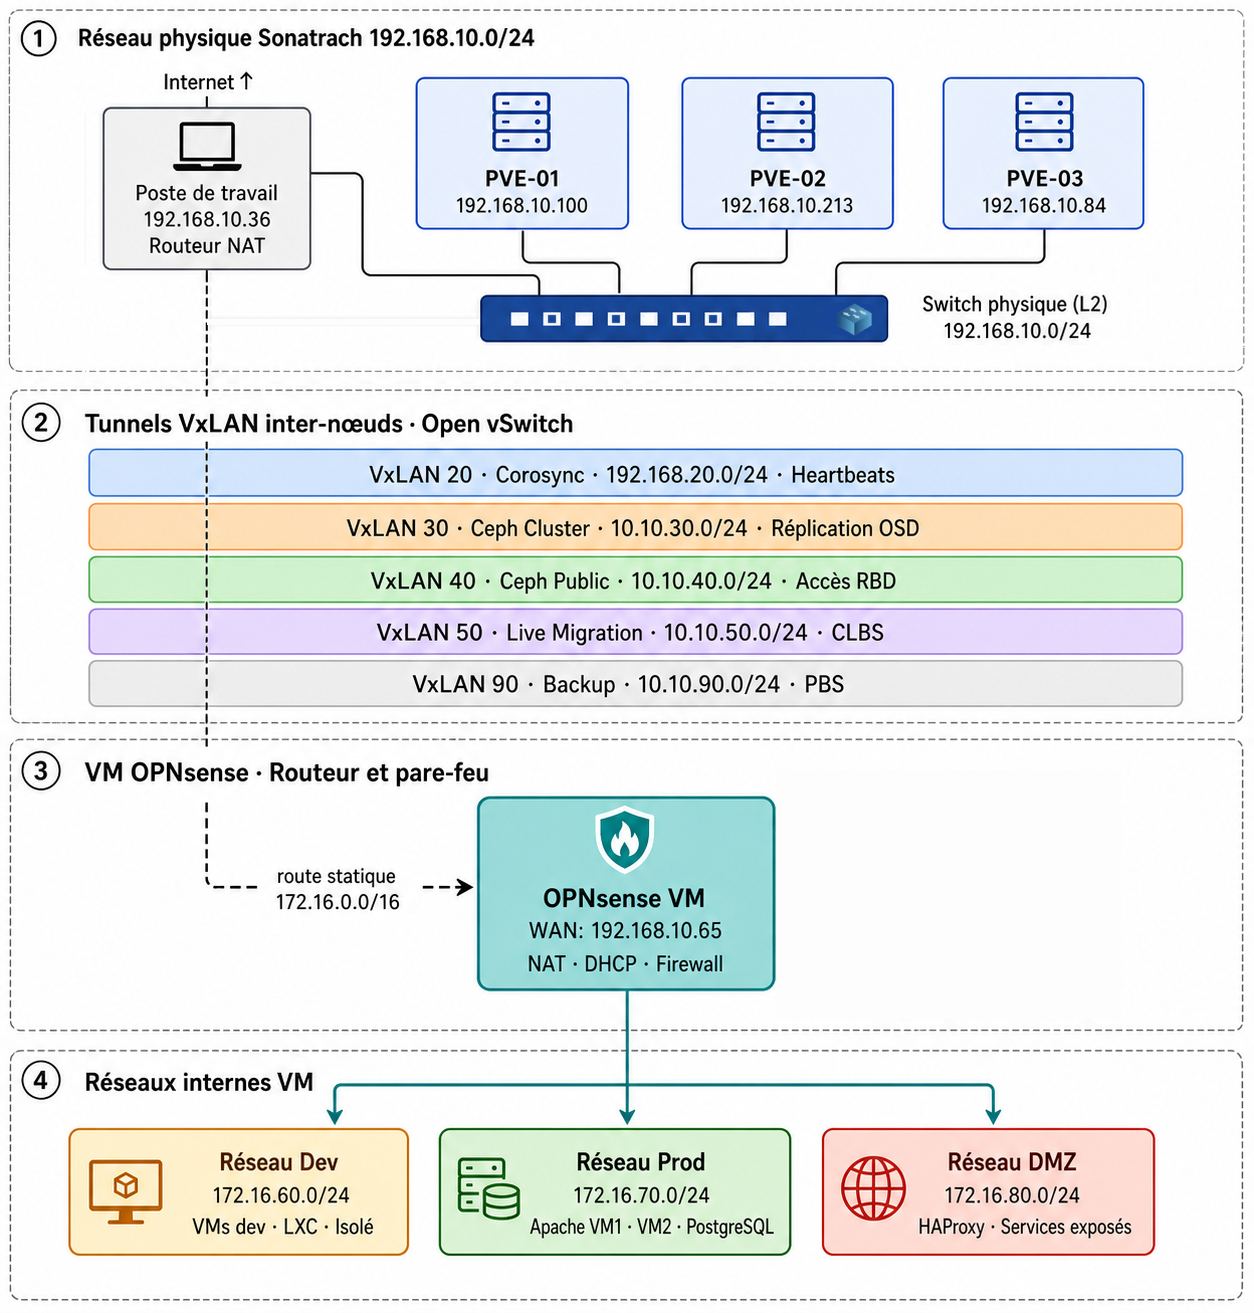
\includegraphics[width=0.9\textwidth]{image/ch3/architecture reseau.png}
        \caption{Topologie Réseau et Plan VxLAN}
        \label{fig:topologie-reseau}
    \end{center}
\end{figure}

{\color{bleuu} \subsection{Bridges Open vSwitch par N\oe{}ud}}

\par Chaque n\oe{}ud Proxmox expose quatre bridges Open vSwitch identiques, constituant les points d'attachement réseau pour toutes les VMs et les tunnels VxLAN. Le tableau suivant décrit leur rôle et leur configuration :\\

\begin{center}
\begin{tabular}{|p{2.5cm}|p{3cm}|p{3cm}|p{5cm}|}
\hline
\textbf{Bridge OVS} & \textbf{VxLAN associé} & \textbf{Sous-réseau} & \textbf{Rôle} \\
\hline
\texttt{vmbr0} & réseau physique natif & 192.168.10.0/24 & Bridge principal. Accès management, SSH, Web UI Proxmox, monitoring, interface WAN d'OPNsense.\\
\hline
\texttt{vmbr60} & \texttt{vxlan60-int} & 172.16.60.0/24 & Réseau Dev. OPNsense y expose son interface LAN1. \\
\hline
\texttt{vmbr70} & \texttt{vxlan70-int} & 172.16.70.0/24 & Réseau Prod. OPNsense y expose son interface LAN2. \\
\hline
\texttt{vmbr80} & \texttt{vxlan80-int} & 172.16.80.0/24 & Réseau DMZ. OPNsense y expose son interface LAN3. \\
\hline
\end{tabular}
\end{center}
\noindent \textit{Tableau 3-X : Bridges OVS et tunnels VxLAN par n\oe{}ud Proxmox}\\

\par Les interfaces \texttt{vxlan60-int}, \texttt{vxlan70-int} et \texttt{vxlan80-int} sont des ports VxLAN OVS point-à-multipoint établis entre les trois n\oe{}uds, permettant à une VM connectée à \texttt{vmbr60} sur PVE-01 de communiquer de manière transparente avec une VM connectée au même bridge sur PVE-02 ou PVE-03, sans aucune configuration supplémentaire au niveau de la VM.\\

{\color{bleuu} \subsection{Plan d'Adressage}}

\par Le plan d'adressage est organisé en deux familles de réseaux. Les réseaux VxLAN d'infrastructure interconnectent les n\oe{}uds Proxmox entre eux pour les flux de contrôle et de données de la plateforme. Les réseaux applicatifs internes sont gérés par OPNsense et hébergent les VMs et conteneurs.\\

\par \textbf{Réseaux VxLAN d'infrastructure :}
\begin{itemize}
    \item \textbf{VxLAN 10 -- Management (192.168.10.0/24, passerelle 192.168.10.36) :} Web UI Proxmox, SSH, API (réseau physique existant).
    \item \textbf{VxLAN 20 -- Corosync (192.168.20.0/24) :} Heartbeats et quorum cluster.
    \item \textbf{VxLAN 30 -- Ceph Cluster (10.10.30.0/24) :} Réplication OSD interne.
    \item \textbf{VxLAN 40 -- Ceph Public (10.10.40.0/24) :} Accès VMs au stockage RBD.
    \item \textbf{VxLAN 50 -- Live Migration (10.10.50.0/24) :} Migrations à chaud et CLBS.
\end{itemize}

\par \textbf{Réseaux applicatifs internes (gérés par OPNsense) :}
\begin{itemize}
    \item \textbf{Réseau Dev (172.16.60.0/24, passerelle OPNsense LAN1 172.16.60.1) :} environnements de développement et de test.
    \item \textbf{Réseau Prod (172.16.70.0/24, passerelle OPNsense LAN2 172.16.70.1) :} environnements de production.
    \item \textbf{Réseau DMZ (172.16.80.0/24, passerelle OPNsense LAN3 172.16.80.1) :} services exposés, dont HAProxy.
\end{itemize}

\begin{center}
\begin{tabular}{|p{1.8cm}|p{2.8cm}|p{2.5cm}|p{2.5cm}|p{2.5cm}|p{2.5cm}|}
\hline
\textbf{N\oe{}ud} & \textbf{Management} & \textbf{VxLAN 20 Corosync} & \textbf{VxLAN 30 Ceph Cluster} & \textbf{VxLAN 40 Ceph Public} & \textbf{VxLAN 50 Migration} \\
\hline
PVE-01 & 192.168.10.100 & 192.168.20.11 & 10.10.30.11 & 10.10.40.11 & 10.10.50.11 \\
\hline
PVE-02 & 192.168.10.213 & 192.168.20.12 & 10.10.30.12 & 10.10.40.12 & 10.10.50.12 \\
\hline
PVE-03 & 192.168.10.84  & 192.168.20.13 & 10.10.30.13 & 10.10.40.13 & 10.10.50.13 \\
\hline
\end{tabular}
\end{center}
\noindent \textit{Tableau 3-3 : Adressage IP statique des n\oe{}uds Proxmox par réseau logique}\\

{\color{bleuu} \subsection{VM OPNsense : Routeur et Pare-feu Centralisé}}

\par La VM OPNsense constituera le coeur du réseau applicatif. Il s'agit d'une distribution FreeBSD dédiée aux fonctions de routage et de sécurité réseau, reconnue pour sa richesse fonctionnelle et sa robustesse en environnement virtualisé. Dans notre architecture, OPNsense sera déployée avec quatre interfaces réseau virtuelles :

\begin{itemize}
    \item \textbf{Interface WAN (192.168.10.65/24) :} connectée au bridge OVS du réseau de management, avec la passerelle 192.168.10.36 (routeur externe). Cette interface assure l'accès Internet sortant via NAT pour toutes les VMs internes.
    \item \textbf{Interface LAN1 (172.16.60.1/24) :} passerelle du réseau Dev.
    \item \textbf{Interface LAN2 (172.16.70.1/24) :} passerelle du réseau Prod.
    \item \textbf{Interface LAN3 (172.16.80.1/24) :} passerelle du réseau DMZ.
\end{itemize}

\par OPNsense intègre nativement dnsmasq, que nous utiliserons comme serveur DHCP pour les trois réseaux internes. L'attribution d'adresses IP aux VMs et conteneurs sera ainsi automatisée dès leur connexion à l'un des bridges applicatifs, ce qui simplifiera le provisionnement dans les playbooks Ansible.\\

{\color{bleuu} \subsection{Haute Disponibilité d'OPNsense}}

\par OPNsense étant le point central du routage inter-réseaux et du
filtrage applicatif, sa défaillance isolerait l'ensemble des réseaux
internes. Dans notre architecture, la résilience d'OPNsense est
assurée par son intégration au groupe HA Proxmox (\texttt{sona-ha-group}).\\

\par En cas de défaillance du n\oe{}ud hébergeant la VM OPNsense,
Corosync détecte la panne et le HA Manager de Proxmox déclenche
automatiquement le redémarrage de la VM sur l'un des deux n\oe{}uds
survivants. La VM redémarre directement depuis son volume Ceph RBD,
sans transfert de données préalable, ce qui minimise le temps de
reprise. Ce délai de basculement est typiquement compris entre 60 et
120 secondes, pendant lesquels le trafic inter-réseaux est interrompu.\\

\par Cette approche offre une reprise automatique après panne sans
nécessiter de déploiement d'une seconde instance OPNsense. Elle
constitue un compromis adapté au contexte de notre infrastructure de
démonstration : le RTO de 60 à 120 secondes est acceptable pour les
scénarios de validation visés. Une architecture de production
nécessitant un basculement transparent pourrait évoluer vers une
configuration active/passive avec le protocole CARP, natif dans
OPNsense, qui réduirait ce délai à moins de 5 secondes.\\

% ============================================================
{\color{bleu} \section{Architecture du Pare-feu}}
% ============================================================

\par La conception du pare-feu s'articule sur deux niveaux complémentaires : le pare-feu applicatif centralisé dans OPNsense, et le pare-feu d'hyperviseur natif de Proxmox VE. Cette complémentarité est illustrée en figure 3-3.\\

{\color{bleuu} \subsection{Pare-feu OPNsense : Filtrage Inter-réseaux}}

\par OPNsense appliquera les politiques de filtrage entre les réseaux applicatifs Dev, Prod et DMZ, ainsi que les règles d'accès Internet. Les règles retenues pour notre conception sont les suivantes :\\

\textbf{Règles autorisées :}
\begin{itemize}
    \item Dev vers WAN (Internet) : autorisé pour les mises à jour et les dépôts de paquets.
    \item DMZ vers WAN (Internet) : autorisé pour les services exposés nécessitant un accès sortant.
    \item Prod vers DMZ : autorisé afin de permettre aux services de production de communiquer avec les composants exposés (HAProxy, etc.).
\end{itemize}

\textbf{Règles bloquées :}
\begin{itemize}
    \item Dev vers Prod : bloqué. Les environnements de développement ne doivent pas avoir accès direct aux ressources de production.
    \item Dev vers DMZ : bloqué. Les services de développement ne doivent pas être accessibles ou accéder aux services exposés publiquement.
    \item Prod vers WAN direct : bloqué. Le trafic de production à destination d'Internet passera obligatoirement par la DMZ.
\end{itemize}

{\color{bleuu} \subsection{Pare-feu Proxmox : Filtrage au Niveau Hyperviseur}}

\par Proxmox VE intègre nativement un mécanisme de pare-feu basé sur iptables, configurable à trois niveaux : cluster, n\oe{}ud et VM individuelle [6]. Nous exploiterons ce mécanisme pour une couche de protection complémentaire au niveau de l'hyperviseur, indépendante d'OPNsense.\\

\par Au niveau du cluster, nous définirons un ensemble de règles globales visant à protéger les interfaces de management et à isoler les réseaux d'infrastructure. Les règles de conception retenues sont les suivantes :

\begin{itemize}
    \item \textbf{Isolation des réseaux Ceph :} interdire tout trafic provenant des réseaux applicatifs (172.16.x.0/24) à destination des réseaux Ceph Cluster (VxLAN 30) et Ceph Public (VxLAN 40). Ces réseaux sont réservés à l'usage exclusif des n\oe{}uds Proxmox.
    \item \textbf{Isolation du réseau Corosync :} interdire tout accès extérieur au réseau VxLAN 20. Seuls les n\oe{}uds Proxmox communiqueront sur ce réseau.
    \item \textbf{Protection de l'interface de management :} restreindre l'accès à l'interface web Proxmox (port 8006) et SSH (port 22) aux seules adresses du sous-réseau 192.168.10.0/24.
    \item \textbf{Limitation des accès inter-VMs :} au niveau de chaque VM, n'autoriser que les ports applicatifs nécessaires, en suivant le principe du moindre privilège.
\end{itemize}

\begin{figure}[H]
    \begin{center}
        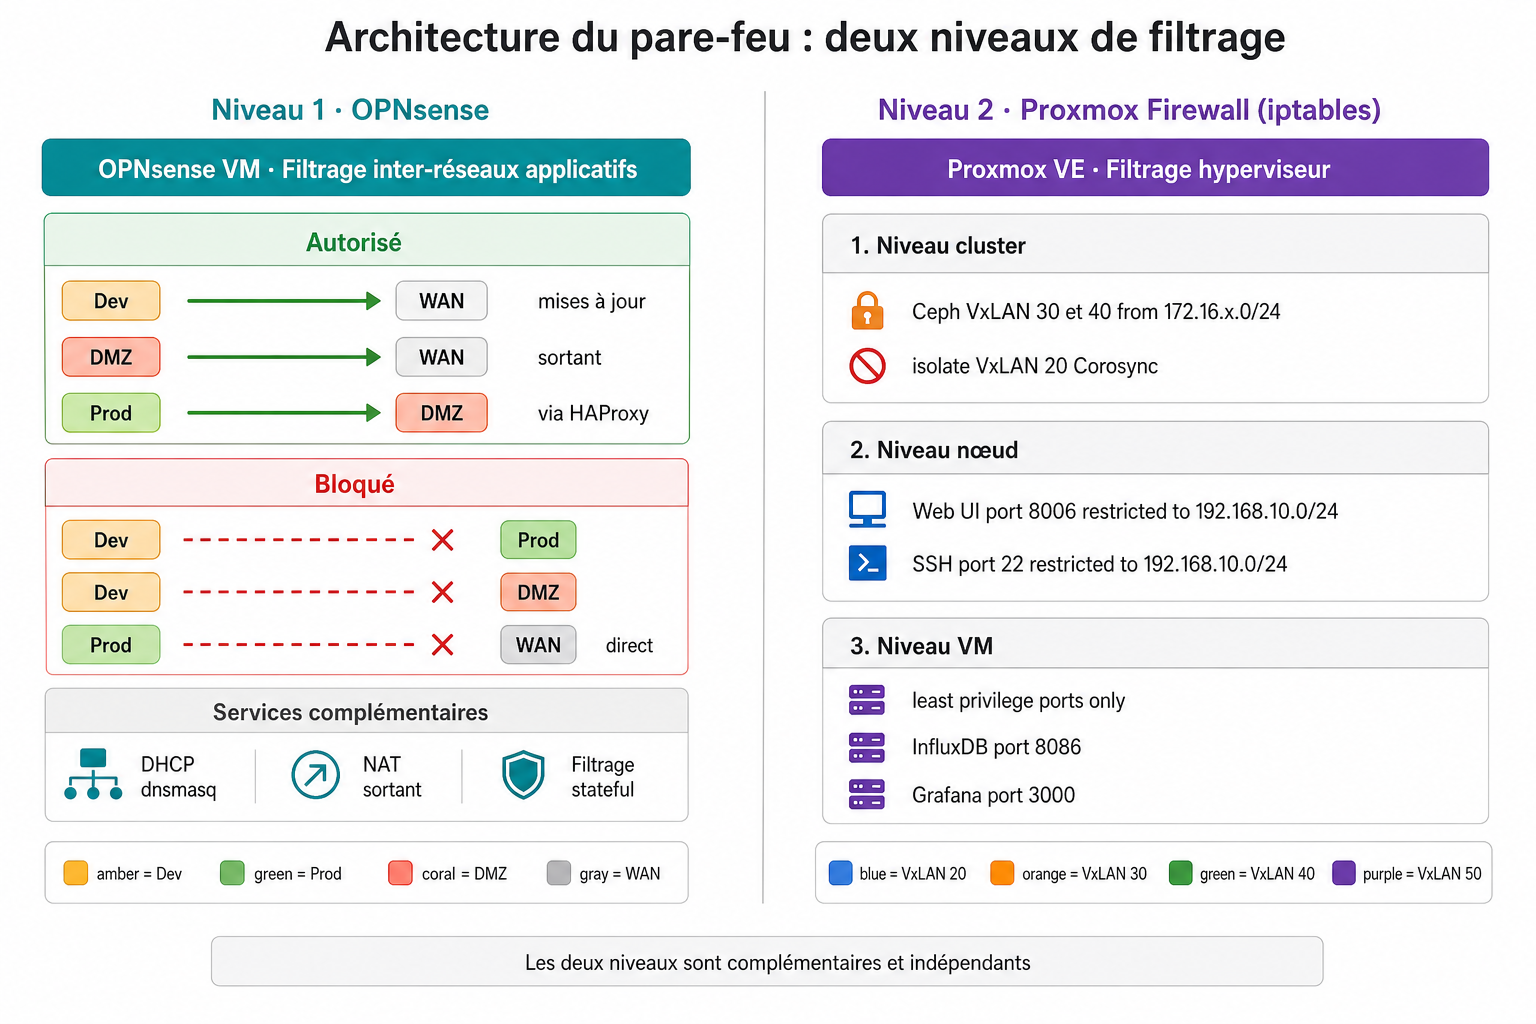
\includegraphics[width=0.9\textwidth]{image/ch3/firewall.png}
        \caption{Architecture du Pare-feu : OPNsense et Proxmox Firewall}
        \label{fig:firewall}
    \end{center}
\end{figure}


% %%%%%%%%%%%%%%%%%%%%%%%%%%%%%%%%%%%%%%%%%%%%%%%%%%%%%%%%%%%%
% CONCLUSION
% %%%%%%%%%%%%%%%%%%%%%%%%%%%%%%%%%%%%%%%%%%%%%%%%%%%%%%%%%%%%

% ============================================================
{\color{bleu} \section{Conclusion}}
% ============================================================

\par Ce chapitre a présenté la conception complète de l'infrastructure Cloud privée hyperconvergée proposée, organisée autour des trois piliers fondamentaux de l'HCI. La partie Compute couvre les trois n\oe{}uds physiques Proxmox bare metal sur serveurs Dell PowerEdge R720, le cluster Proxmox avec son mécanisme de quorum Corosync et de haute disponibilité, le mécanisme d'équilibrage proactif CLBS adapté du CSLB, l'application de démonstration Sona-Web, ainsi que l'automatisation via Ansible et PXE. La partie Storage détaille le cluster Ceph avec ses composants MON/MGR/OSD, le dimensionnement du pool et la politique de thin provisioning. La partie Network expose l'architecture VxLAN inter-noeuds gérée par Open vSwitch, le plan d'adressage complet, le routage centralisé via OPNsense, et le plan de pare-feu à deux niveaux. L'ensemble de ces choix de conception constitue une base cohérente et documentée pour la phase d'implémentation présentée dans le chapitre suivant.\\
{\color{bleu}\chapter{Implémentation de la Solution Proposée}}
\thispagestyle{empty}
\newpage

% =========================
% Packages needed in preamble
% =========================
% \usepackage{float}
% \usepackage{xcolor}
% \usepackage{graphicx}
% \usepackage{caption}
% \usepackage{listings}
%
% \definecolor{codebg}{RGB}{245,245,244}
% \definecolor{codeframe}{RGB}{210,210,210}
% \definecolor{codecomment}{RGB}{0,128,0}
% \definecolor{codekeyword}{RGB}{0,0,180}
% \definecolor{codestring}{RGB}{163,21,21}
%
% \lstdefinestyle{sonacode}{
%     backgroundcolor=\color{codebg},
%     frame=single,
%     rulecolor=\color{codeframe},
%     basicstyle=\ttfamily\small,
%     keywordstyle=\color{codekeyword}\bfseries,
%     commentstyle=\color{codecomment},
%     stringstyle=\color{codestring},
%     breaklines=true,
%     showstringspaces=false,
%     tabsize=2,
%     captionpos=b
% }

{\color{bleu} \section{Introduction}}

\par Ce chapitre présente la mise en œuvre concrète de la solution proposée dans le chapitre précédent. L’objectif est de montrer les étapes réelles de déploiement de l’infrastructure hyperconvergée, depuis l’installation de la plateforme de virtualisation jusqu’aux services applicatifs et aux mécanismes d’automatisation. Pour améliorer la lisibilité, l’implémentation est organisée en trois grandes parties : la couche calcul, la couche stockage, puis la couche réseau.\\

\par Les opérations ont été réalisées avec plusieurs outils complémentaires : l’interface web Proxmox VE, la ligne de commande Linux, les fichiers de configuration système, OPNsense, Ceph, ainsi que des playbooks Ansible pour automatiser certaines tâches répétitives. Des captures d’écran sont prévues aux points importants afin d’illustrer visuellement les résultats obtenus.\\

{\color{bleu} \section{Partie I --- Couche Calcul}}

{\color{bleuu} \subsection{Préparation de l’Infrastructure Physique}}

{\color{bleuuu} \subsubsection{Installation de Proxmox VE sur les nœuds}}

\par L’installation de la plateforme de virtualisation a commencé par le téléchargement de l’image ISO de Proxmox VE version 9.1.1. Cette image a ensuite été copiée sur une clé USB bootable utilisée pour démarrer chaque serveur Dell PowerEdge R720. Une installation séparée a été réalisée sur chacun des trois nœuds du cluster.\\

\par Pendant l’installation, le disque système \texttt{sda} a été utilisé pour héberger Proxmox VE. Une configuration réseau statique a aussi été appliquée afin de donner à chaque nœud une adresse de management fixe sur le réseau physique \texttt{192.168.10.0/24}. Les adresses retenues sont \texttt{192.168.10.100} pour PVE-01, \texttt{192.168.10.213} pour PVE-02 et \texttt{192.168.10.84} pour PVE-03.\\

\par Une fois l’installation terminée, la vérification a été effectuée à travers l’interface web de Proxmox, accessible sur le port \texttt{8006}. Cette étape a permis de confirmer que chaque nœud était opérationnel et prêt pour la suite du déploiement.\\

\begin{figure}[H]
    \centering
    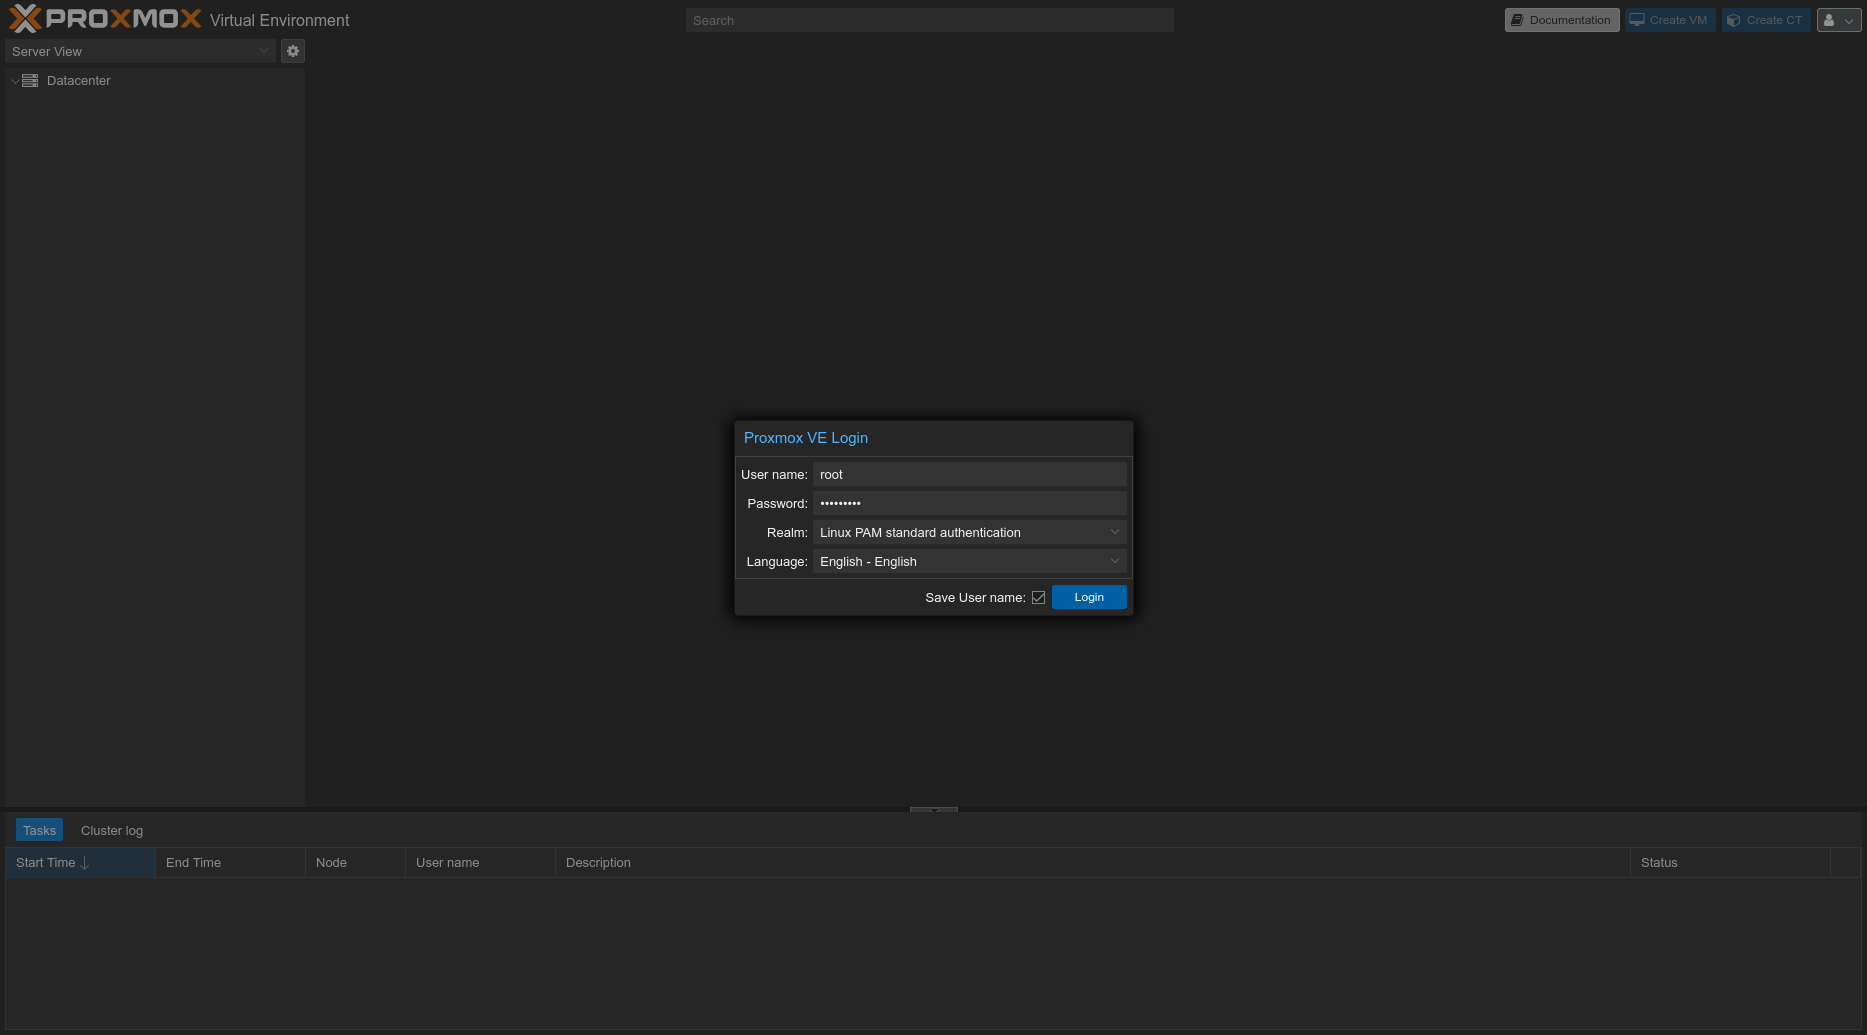
\includegraphics[width=0.9\textwidth]{image/ch4/proxmox.png}
    \caption{Interface web Proxmox au premier login sur PVE-01}
    \label{fig:proxmox-first-login}
\end{figure}

{\color{bleuuu} \subsubsection{Configuration de la connectivité Internet via le laptop gateway}}

\par Dans l’environnement de laboratoire, aucun routeur physique dédié n’était disponible pour fournir l’accès Internet aux nœuds Proxmox. Pour cette raison, un laptop a été configuré pour jouer le rôle de passerelle NAT entre le réseau interne de l’infrastructure et Internet. Il possède deux interfaces : \texttt{enp0s20f0u4c2} côté infrastructure avec l’adresse \texttt{192.168.10.36/24}, et \texttt{wlan0} côté Internet avec l’adresse \texttt{10.247.78.8/24}.\\

\par La première étape consiste à activer le routage IP afin que le système puisse transférer les paquets d’une interface à l’autre. Cette activation doit être faite de manière immédiate puis rendue permanente.\\

\begin{lstlisting}[style=sonacode,language=bash,caption={Activation du routage IP sur le laptop},label={lst:ipforward}]
sudo sysctl -w net.ipv4.ip_forward=1
sudo vim /etc/sysctl.d/99-ipforward.conf
# Ajouter :
net.ipv4.ip_forward=1
\end{lstlisting}

\par Ensuite, des règles \texttt{iptables} ont été ajoutées pour réaliser la translation d’adresses NAT et autoriser le forwarding du trafic entre les interfaces du laptop.\\

\begin{lstlisting}[style=sonacode,language=bash,caption={Configuration NAT avec iptables},label={lst:iptables-nat}]
sudo iptables -t nat -A POSTROUTING -o wlan0 -j MASQUERADE
sudo iptables -A FORWARD -i enp0s20f0u4c2 -o wlan0 -j ACCEPT
sudo iptables -A FORWARD -i wlan0 -o enp0s20f0u4c2 -m state --state RELATED,ESTABLISHED -j ACCEPT
\end{lstlisting}

\par Pour éviter de perdre ces règles après redémarrage, elles ont été sauvegardées puis activées automatiquement au boot du laptop.\\

\begin{lstlisting}[style=sonacode,language=bash,caption={Persistance des règles iptables},label={lst:iptables-persist}]
sudo pacman -S iptables-nft
sudo iptables-save | sudo tee /etc/iptables/iptables.rules
sudo systemctl enable iptables
\end{lstlisting}

\par Sur chaque nœud Proxmox, la passerelle par défaut a été définie vers \texttt{192.168.10.36}, avec des serveurs DNS publics. Cette configuration a été ajoutée dans le fichier \texttt{/etc/network/interfaces}.\\

\begin{lstlisting}[style=sonacode,language={},caption={Configuration réseau de base d’un nœud Proxmox},label={lst:proxmox-basic-network}]
auto vmbr0
iface vmbr0 inet static
    address 192.168.10.XX/24
    gateway 192.168.10.36
    dns-nameservers 8.8.8.8 8.8.4.4
\end{lstlisting}

\par Enfin, des routes statiques ont été ajoutées sur le laptop afin de rediriger les réseaux internes \texttt{172.16.60.0/24}, \texttt{172.16.70.0/24} et \texttt{172.16.80.0/24} vers la VM OPNsense, qui assure ensuite le routage vers ces sous-réseaux.\\

\begin{lstlisting}[style=sonacode,language=bash,caption={Ajout des routes statiques vers OPNsense},label={lst:static-routes-opnsense}]
nmcli connection modify "Wired connection 1" \
 +ipv4.routes "172.16.60.0/24 192.168.10.65" \
 +ipv4.routes "172.16.70.0/24 192.168.10.65" \
 +ipv4.routes "172.16.80.0/24 192.168.10.65"

nmcli connection up "Wired connection 1"
\end{lstlisting}

\par Des tests simples comme \texttt{ping 8.8.8.8}, \texttt{ping google.com} et \texttt{apt update} ont confirmé que les nœuds disposaient correctement d’un accès Internet.\\

{\color{bleuu} \subsection{Formation du cluster Proxmox et haute disponibilité}}

{\color{bleuuu} \subsubsection{Création et jonction au cluster}}

\par Après l’installation de Proxmox VE sur les trois serveurs, la phase suivante a consisté à former un cluster unique. Cette opération a été lancée depuis le premier nœud PVE-01, qui devient le nœud initial du cluster.\\

\begin{lstlisting}[style=sonacode,language=bash,caption={Création du cluster Proxmox},label={lst:pvecm-create}]
pvecm create Cluster-Proxmox-VE
\end{lstlisting}

\par Les deux autres nœuds ont ensuite rejoint ce cluster en utilisant l’adresse IP du nœud principal.\\

\begin{lstlisting}[style=sonacode,language=bash,caption={Jonction de PVE-02 et PVE-03 au cluster},label={lst:pvecm-add}]
pvecm add 192.168.10.100
\end{lstlisting}

\par Le réseau Corosync, utilisé pour le heartbeat entre les nœuds, a été isolé sur le VxLAN 20 afin de séparer le trafic de cluster du reste du trafic d’administration ou de production. Une fois la configuration terminée, la commande de vérification a confirmé la présence des trois nœuds avec quorum atteint.\\

\begin{lstlisting}[style=sonacode,language=bash,caption={Vérification de l’état du cluster},label={lst:pvecm-status}]
pvecm status
\end{lstlisting}

\begin{figure}[H]
    \centering
    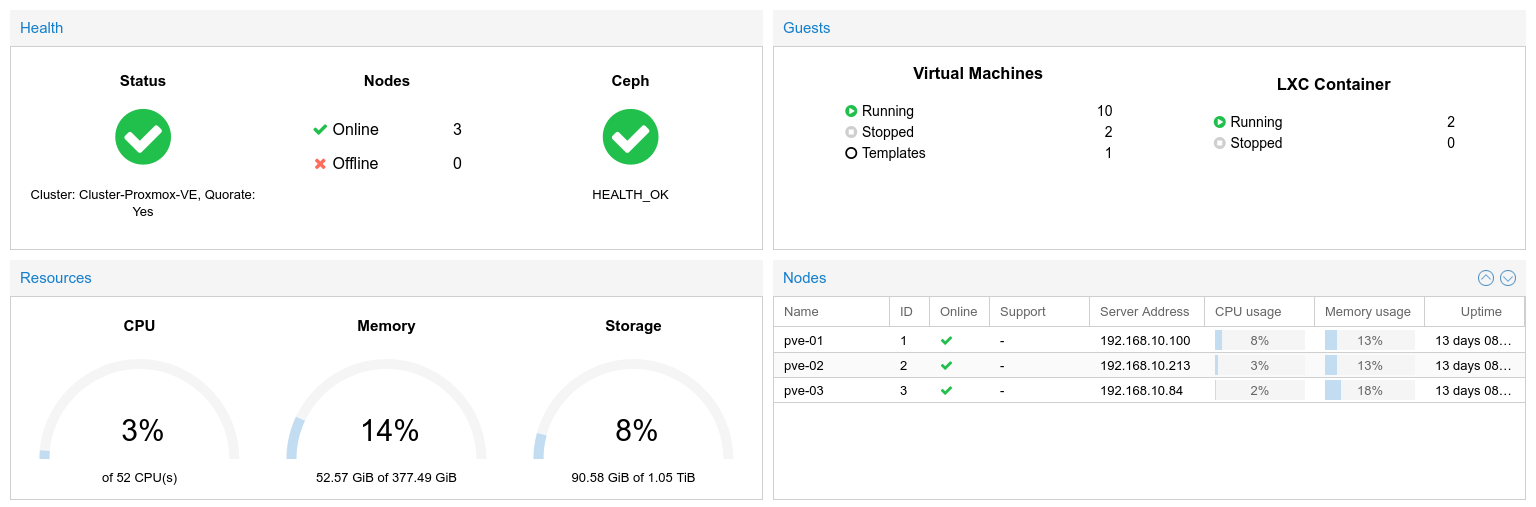
\includegraphics[width=0.9\textwidth]{image/ch4/nodes online.png}
    \caption{Vue du cluster Proxmox montrant les trois nœuds en ligne}
    \label{fig:cluster-three-nodes}
\end{figure}

{\color{bleuuu} \subsubsection{Configuration de la migration à chaud}}

\par La migration à chaud des machines virtuelles a été configurée pour utiliser le réseau dédié VxLAN 50. Ce choix permet de ne pas mélanger le trafic de migration avec le trafic utilisateur ou le trafic de stockage.\\

\par Dans la configuration du datacenter Proxmox, les paramètres de migration ont été ajustés pour utiliser un réseau spécifique et garder un niveau de sécurité acceptable. Une migration manuelle de test a ensuite été réalisée depuis l’interface web afin de vérifier le déplacement transparent d’une VM d’un nœud à un autre sans interruption notable du service.\\

\begin{figure}[H]
    \centering
    
\includegraphics[width=0.9\textwidth]{image/ch4/before migration.png}
    \caption{Avant et après une migration live d’une machine virtuelle}
    \label{fig:live-migration-before-after}
\end{figure}
\begin{figure}[H]
    \centering
    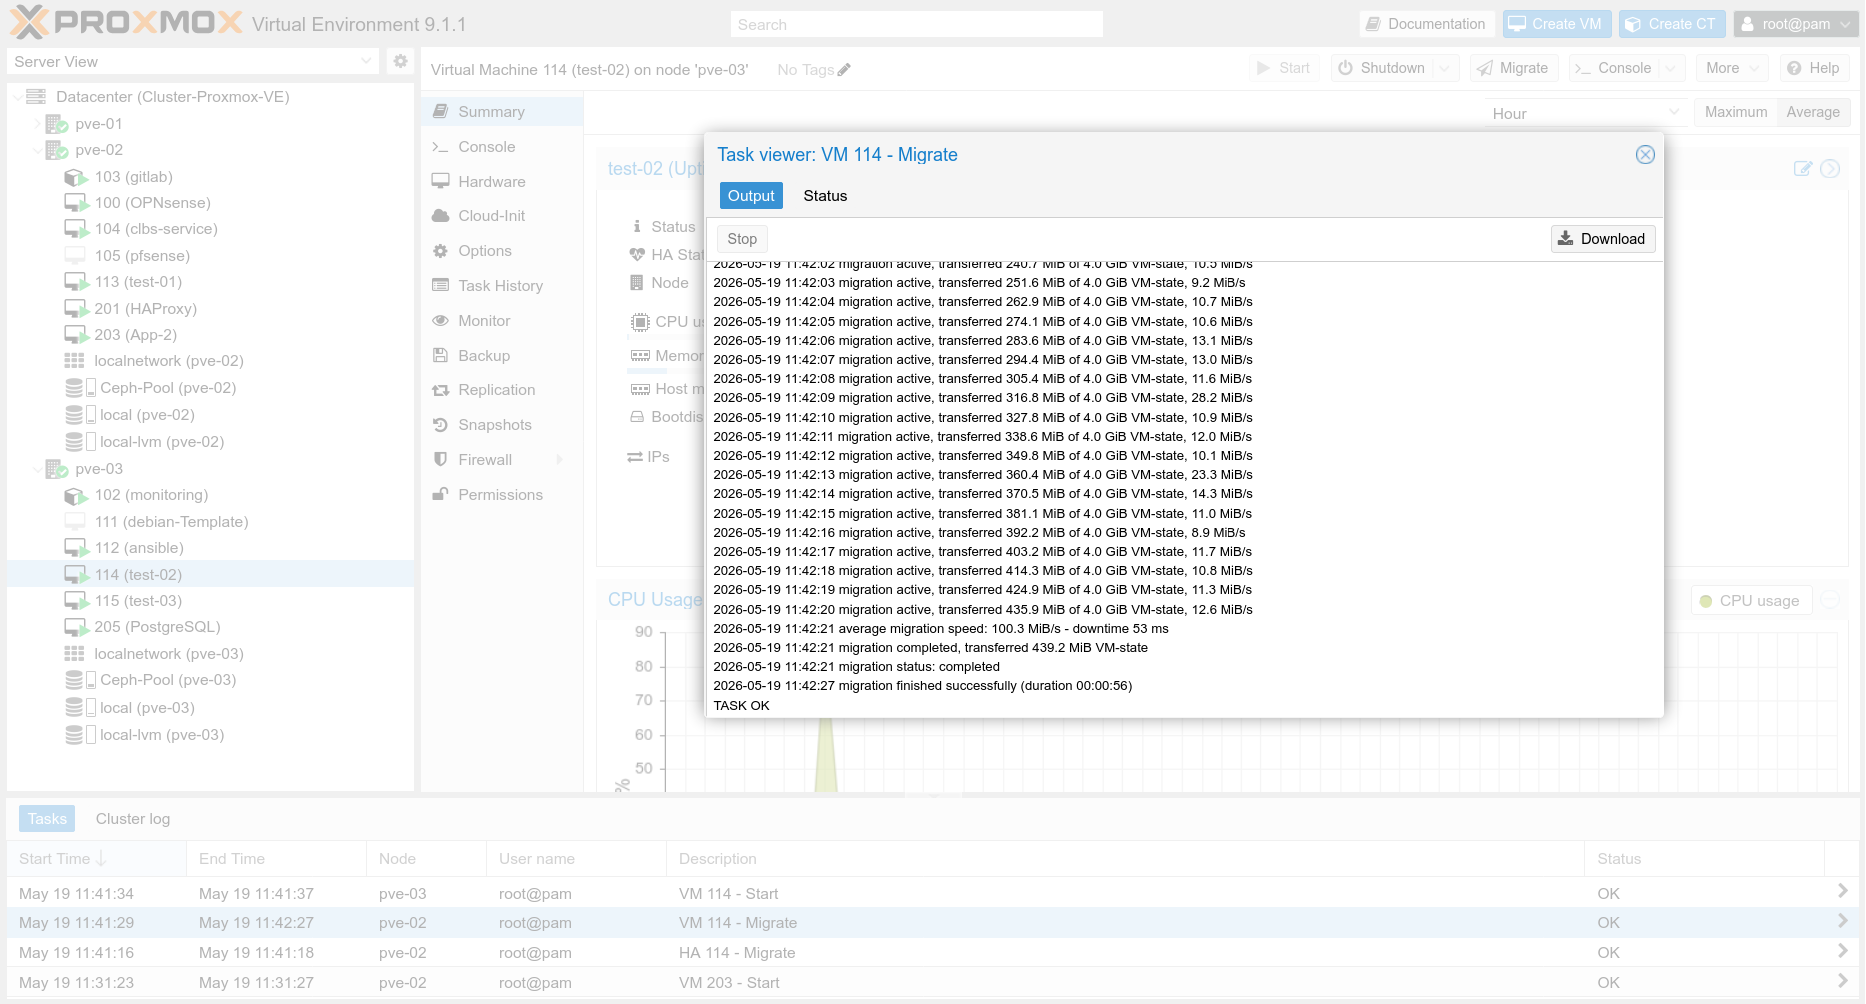
\includegraphics[width=0.9\textwidth]{image/ch4/after migration.png}
    \caption{Avant et après une migration live d’une machine virtuelle}
    \label{fig:live-migration-before-after}
\end{figure}

{\color{bleuu} \subsection{Déploiement de la stack de monitoring}}

\par Afin de superviser l’état global de l’infrastructure, une stack de monitoring a été déployée dans un conteneur LXC dédié appelé \texttt{monitoring}, avec l’adresse \texttt{192.168.10.99}. Ce conteneur centralise InfluxDB, Prometheus et Grafana.\\

{\color{bleuuu} \subsubsection{Déploiement d’InfluxDB}}

\par InfluxDB a été installé pour recevoir les métriques envoyées directement par Proxmox à travers le système natif \textit{Metric Server}. Un bucket nommé \texttt{proxmox-metrics} a été créé afin de stocker les mesures CPU, mémoire, réseau et stockage de chaque nœud du cluster.\\

\par Une fois la configuration validée dans l’interface web Proxmox, les métriques ont commencé à être transmises automatiquement sans agent supplémentaire. La présence des séries temporelles dans l’interface InfluxDB a confirmé le bon fonctionnement de ce mécanisme.\\

\begin{figure}[H]
    \centering
    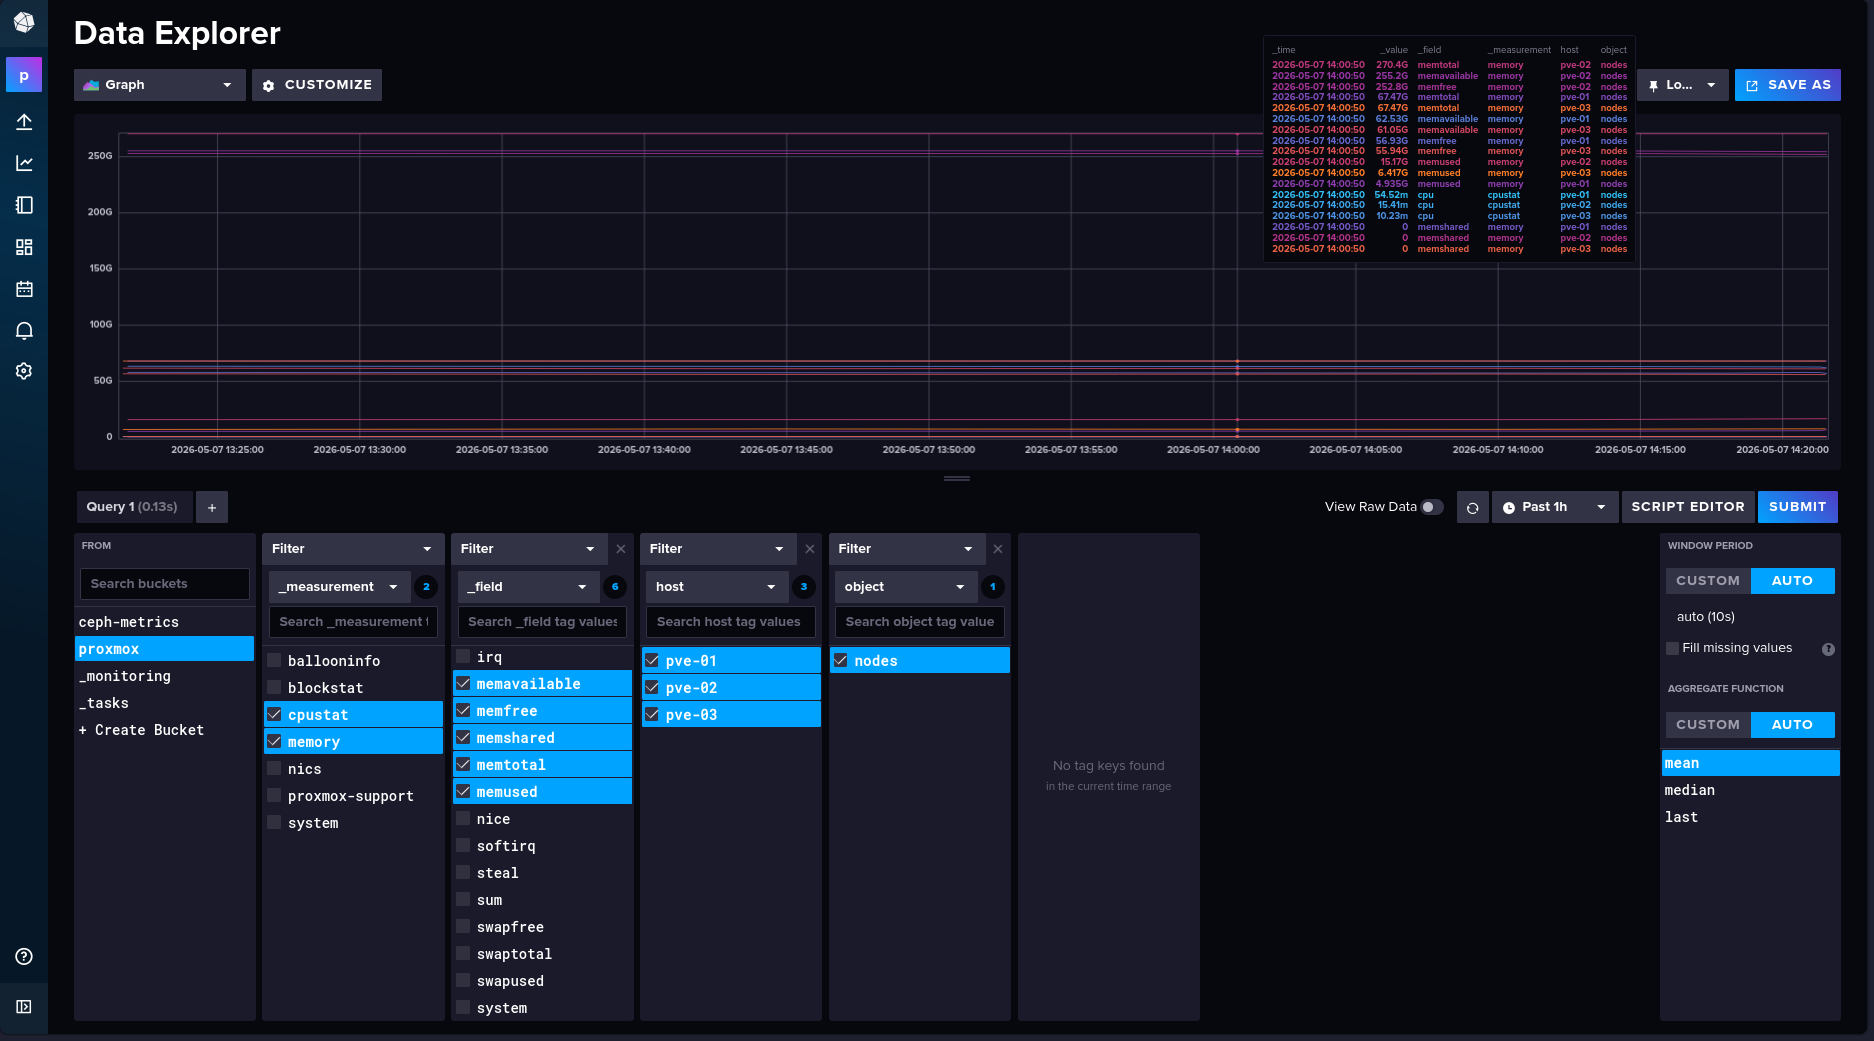
\includegraphics[width=0.9\textwidth]{image/ch4/influxdb.png}
    \caption{Explorateur InfluxDB montrant les métriques reçues depuis Proxmox}
    \label{fig:influxdb-data-explorer}
\end{figure}

{\color{bleuuu} \subsubsection{Déploiement de Prometheus}}

\par Prometheus a été installé dans le même conteneur afin de collecter les métriques exposées par Ceph et par le service applicatif CLBS. La configuration du fichier \texttt{prometheus.yml} contient deux jobs principaux : un job pour les métriques Ceph via le module MGR Prometheus, et un job pour l’application CLBS développée en Go.\\

\begin{lstlisting}[style=sonacode,language=yaml,caption={Extrait du fichier prometheus.yml},label={lst:prometheus-yml}]
global:
  scrape_interval: 30s
  evaluation_interval: 30s

scrape_configs:
  - job_name: ceph
    static_configs:
      - targets:
          - "192.168.10.213:9283"
          - "192.168.10.83:9283"
          - "192.168.10.100:9283"
        labels:
          cluster: "proxmox-lab"

  - job_name: "clbs"
    static_configs:
      - targets: ["192.168.10.104:9101"]
        scrape_interval: 30s
        scrape_timeout: 10s
\end{lstlisting}

\par L’interface web Prometheus a ensuite permis de confirmer que les différentes cibles apparaissaient avec l’état \texttt{UP}.\\

{\color{bleuuu} \subsubsection{Déploiement de Grafana}}

\par Grafana a été ajouté comme couche de visualisation unifiée pour les métriques de Proxmox, Ceph et CLBS. Deux sources de données ont été configurées : InfluxDB pour les métriques de Proxmox, et Prometheus pour les métriques Ceph et applicatives.\\

\begin{table}[H]
\centering
\caption{Dashboards Grafana configurés}
\begin{tabular}{|l|l|l|}
\hline
\textbf{Dashboard} & \textbf{Source} & \textbf{Métriques principales} \\
\hline
Proxmox Cluster & InfluxDB & CPU, RAM, réseau par nœud \\
\hline
Ceph & Prometheus & Santé cluster, pools, latence OSD \\
\hline
CLBS & Prometheus & Historique des migrations \\
\hline
\end{tabular}
\end{table}

\par Trois dashboards principaux ont ainsi été utilisés : un dashboard infrastructure Proxmox, un dashboard Ceph, et un dashboard personnalisé pour le service CLBS.\\

\begin{figure}[H]
    \centering
    \includegraphics[width=0.9\textwidth]{image/ch4/Grafana.png}
    \caption{Dashboard Grafana Infrastructure pour les nœuds Proxmox}
    \label{fig:grafana-proxmox-dashboard}
\end{figure}

{\color{bleuu} \subsection{Implémentation du mécanisme CLBS}}

{\color{bleuuu} \subsubsection{Structure du service}}

\par Le service CLBS (\textit{Cluster Load Balancing Service}) a été développé en langage Go dans une VM dédiée accessible sur le réseau de management. Son rôle est d’analyser périodiquement la charge CPU du cluster et de déclencher automatiquement des migrations live lorsque cela est nécessaire.\\

\par Le code est structuré en plusieurs composants : un lecteur InfluxDB pour les métriques historiques, un client API Proxmox pour piloter le cluster, un calculateur de bandes de charge, et un moteur principal de décision. Les paramètres de connexion sont placés dans un fichier \texttt{.env} chargé au démarrage du service.\\

{\color{bleuuu} \subsubsection{Logique de décision}}

\par À chaque cycle, le service récupère la charge des nœuds, calcule les bornes de charge modérée, puis classe les nœuds dans les catégories \textit{heavy}, \textit{moderate} ou \textit{light}. Si un déséquilibre est détecté entre un nœud surchargé et un nœud léger, le moteur choisit la VM la plus adaptée à migrer.\\

\par Plusieurs mécanismes de protection ont été ajoutés pour éviter les migrations excessives, comme un temps de cooldown global, un cooldown individuel par VM et une suspension temporaire en cas de fréquence de migration trop élevée.\\

{\color{bleuuu} \subsubsection{Déploiement comme service systemd}}

\par Une fois compilé, le binaire Go a été déployé sur la VM CLBS puis intégré comme service \texttt{systemd} afin d’assurer un démarrage automatique et une relance en cas de panne.\\

\begin{lstlisting}[style=sonacode,language=bash,caption={Gestion du service CLBS avec systemd},label={lst:clbs-systemd}]
systemctl enable clbs
systemctl start clbs
journalctl -u clbs.service -f -o cat
\end{lstlisting}

{\color{bleuuu} \subsubsection{Validation du mécanisme}}

\par Pour valider le comportement du service, deux VMs de test ont été créées puis soumises à une charge CPU artificielle avec l’outil \texttt{stress-ng}. Le service CLBS a détecté la surcharge et a déclenché une migration live vers un nœud moins chargé.\\

\begin{lstlisting}[style=sonacode,language=bash,caption={Génération d’une charge CPU de test},label={lst:stress-ng}]
stress-ng --cpu 8
\end{lstlisting}

\begin{figure}[H]
    \centering
    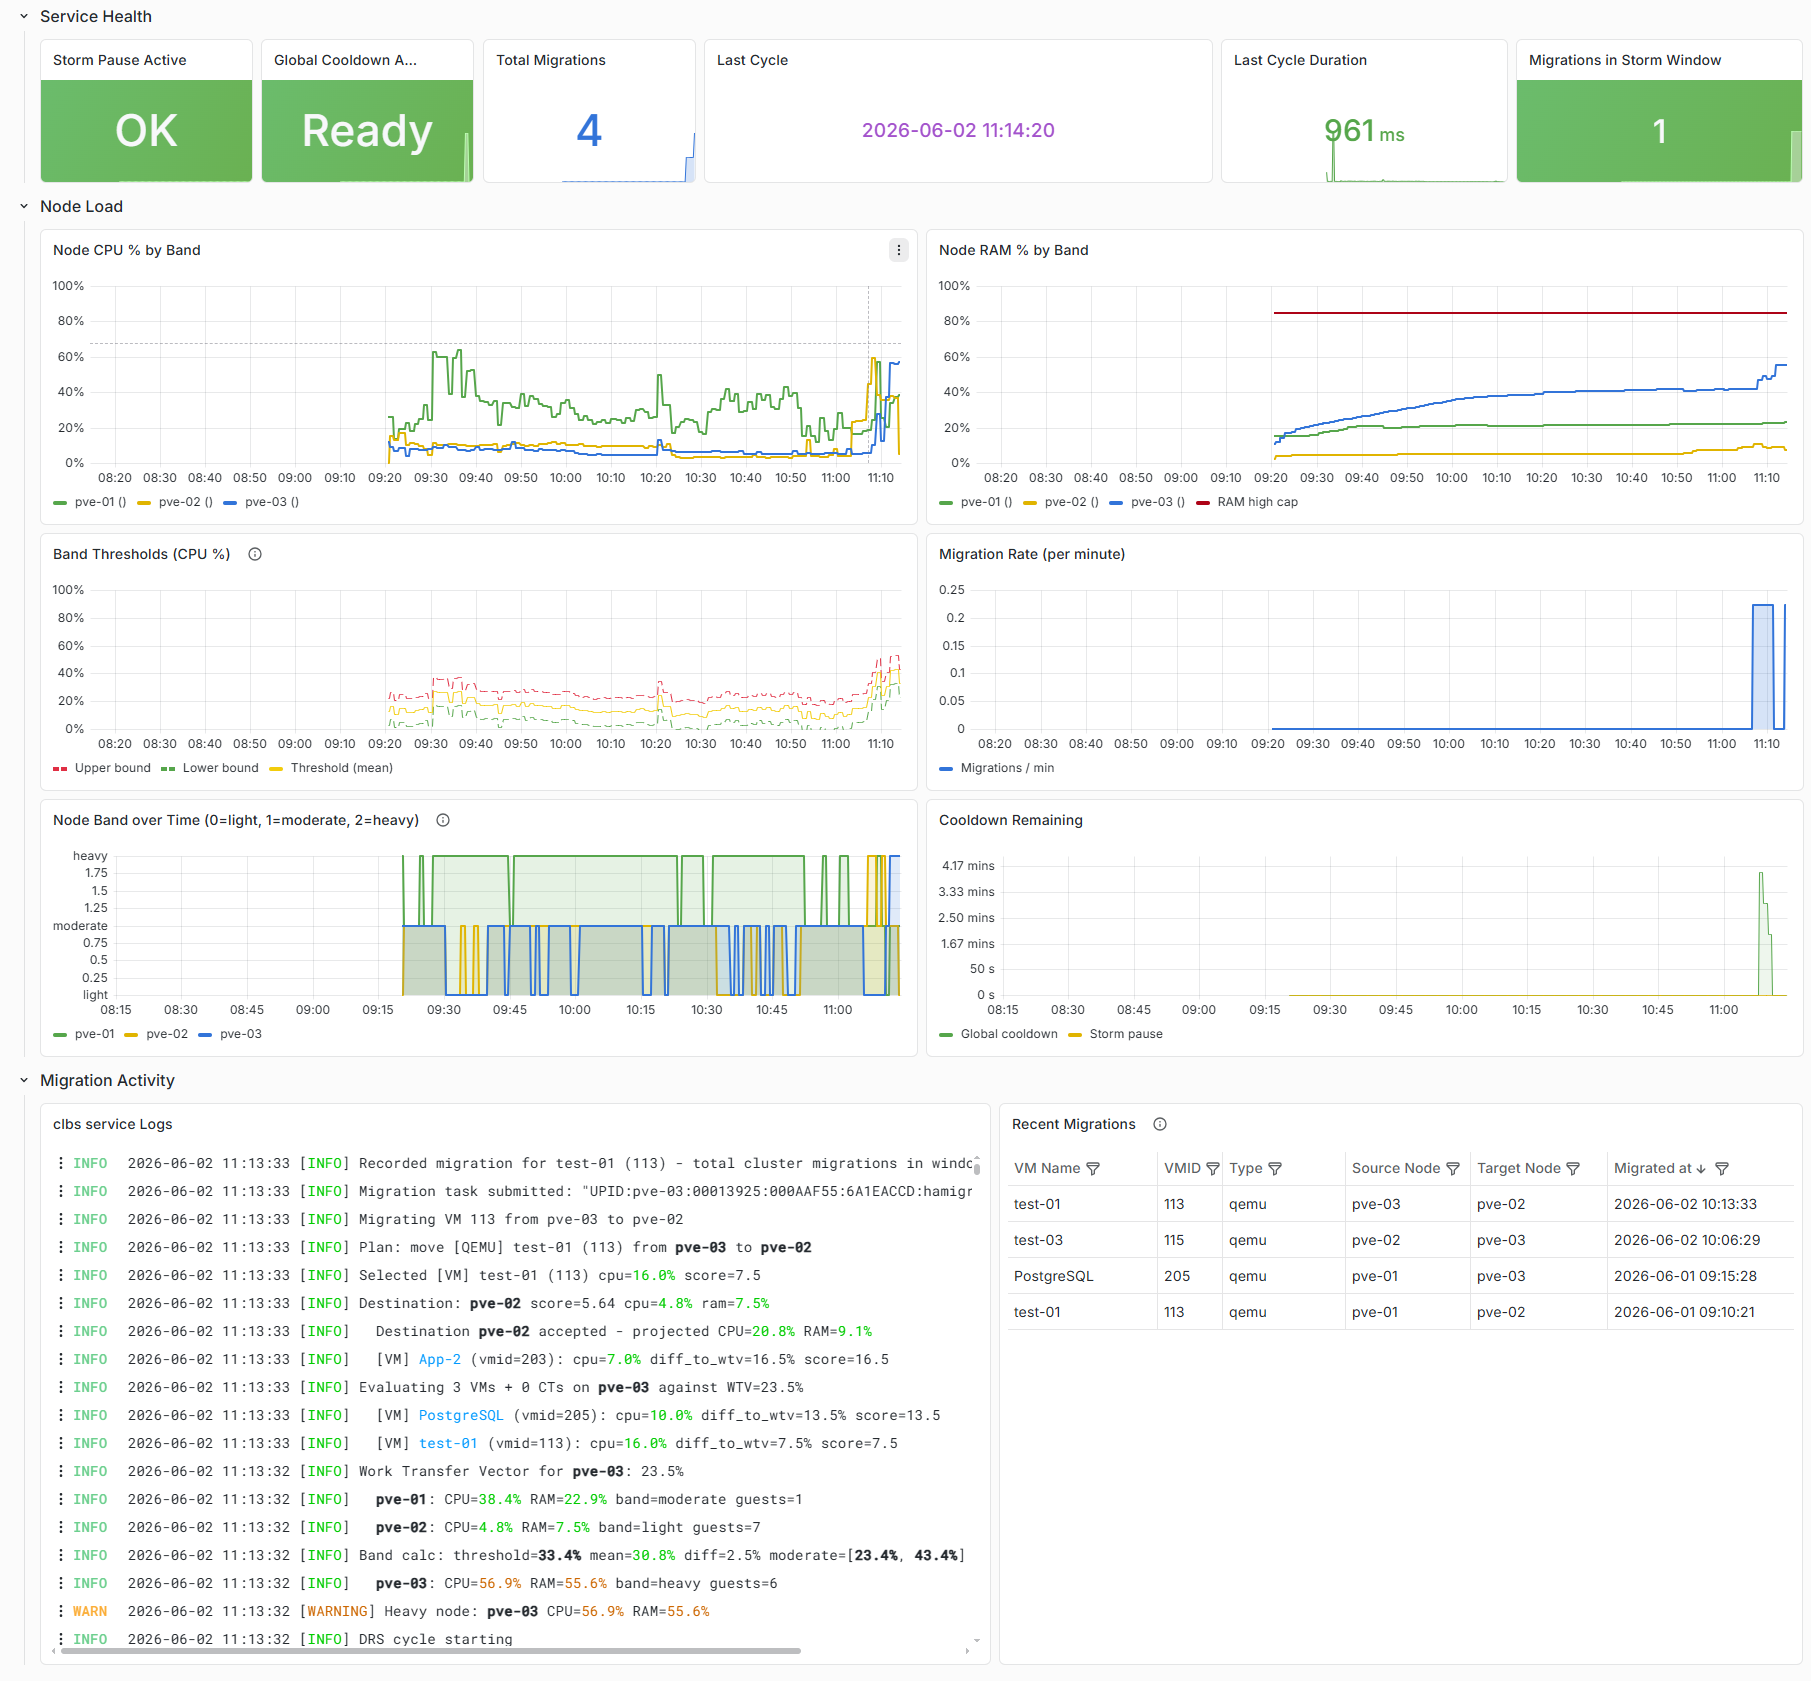
\includegraphics[width=0.9\textwidth]{image/ch4/clbs dashboard.png}
    \caption{Dashboard ou logs montrant une migration déclenchée par CLBS}
    \label{fig:clbs-migration-event}
\end{figure}

{\color{bleuu} \subsection{Déploiement de l’application Sona-Web}}

{\color{bleuuu} \subsubsection{Création des machines virtuelles}}

\par L’application Sona-Web a été déployée sous la forme de plusieurs VMs créées à partir d’un template Debian stocké dans le pool Ceph. Cette architecture comprend une VM HAProxy en frontal, deux VMs Flask pour la couche applicative, et une VM PostgreSQL pour la base de données.\\

\par Les VMs ont été déployées sur les réseaux internes appropriés, avec attribution d’adresse IP par DHCP selon la zone de sécurité visée. Cette organisation permet de séparer la partie exposée, la partie applicative et la base de données.\\

{\color{bleuuu} \subsubsection{Validation de l’application}}

\par La validation a porté sur le fonctionnement du load balancing ainsi que sur la disponibilité de l’application. Des requêtes répétées à travers HAProxy ont montré une alternance correcte entre les serveurs applicatifs Flask, confirmant le bon fonctionnement du mécanisme de répartition de charge.\\

\begin{lstlisting}[style=sonacode,language=bash,caption={Test de répartition HAProxy},label={lst:haproxy-test}]
for i in $(seq 1 10); do
  curl -s http://172.16.80.x | grep "Server"
done
\end{lstlisting}

{\color{bleuu} \subsection{Automatisation avec Ansible}}

{\color{bleuuu} \subsubsection{Environnement et structure du projet}}

\par Afin de simplifier le provisionnement des machines virtuelles et de rendre l’infrastructure plus reproductible, un environnement Ansible a été mis en place. Les connexions se font via SSH depuis les postes des développeurs vers le réseau de management, sans installation d’agent sur les nœuds cibles.\\

\begin{lstlisting}[style=sonacode,language={},caption={Structure du projet Ansible},label={lst:ansible-tree}]
ansible-infra/
├── ansible.cfg
├── secrets.yml
├── inventory/
│   ├── hosts.yml
│   └── proxmox_nodes.yml
└── playbooks/
    ├── provision_vm.yml
    └── provision_vm_batch.yml
\end{lstlisting}

\begin{lstlisting}[style=sonacode,language=ini,caption={Fichier ansible.cfg},label={lst:ansible-cfg}]
[defaults]
inventory            = inventory/hosts.yml
remote_user          = ansible
private_key_file     = ~/.ssh/ansible_ed25519
host_key_checking    = False
interpreter_python   = /usr/bin/python3

[privilege_escalation]
become      = True
become_user = root
\end{lstlisting}

{\color{bleuuu} \subsubsection{Inventaire}}

\par L’inventaire regroupe les nœuds Proxmox, les VMs permanentes, ainsi qu’un groupe dynamique destiné aux nouvelles VMs provisionnées par les playbooks.\\

\begin{lstlisting}[style=sonacode,language=yaml,caption={Extrait de l’inventaire hosts.yml},label={lst:ansible-hosts}]
all:
  children:
    proxmox_nodes:
      hosts:
        pve-01: {ansible_host: 192.168.10.100}
        pve-02: {ansible_host: 192.168.10.213}
        pve-03: {ansible_host: 192.168.10.84}
    vms:
      hosts:
        monitoring:
          ansible_host: 192.168.10.99
    provisioned_vms:
      hosts: {}
\end{lstlisting}

{\color{bleuuu} \subsubsection{Playbook de provisionnement}}

\par Le playbook principal automatise la création d’une VM à partir d’un template Debian déjà préparé. Il configure les ressources matérielles, le réseau, le cloud-init, le démarrage de la VM, puis sa validation après boot.\\

\begin{lstlisting}[style=sonacode,language=bash,caption={Exemple d’utilisation du playbook provision\_vm.yml},label={lst:ansible-vm-create}]
ansible-playbook playbooks/provision_vm.yml \
  -e "vm_id=110 vm_name=web-01"

ansible-playbook playbooks/provision_vm.yml \
  -e "vm_id=115 vm_name=db-01 vm_cores=4 vm_memory=8192"
\end{lstlisting}

\par L’adresse IP de la VM peut être générée automatiquement à partir du VMID pour simplifier le déploiement.\\

\begin{lstlisting}[style=sonacode,language=yaml,caption={Formule d’attribution automatique de l’adresse IP},label={lst:auto-ip-formula}]
vm_ip: "172.16.60.{{ vm_id | int - 90 }}"
\end{lstlisting}

\par La configuration cloud-init repose sur trois commandes successives : attachement du disque cloud-init, injection de la configuration réseau, puis régénération de l’ISO cloud-init.\\

\begin{lstlisting}[style=sonacode,language=bash,caption={Configuration cloud-init d’une VM Proxmox},label={lst:cloud-init-qm}]
qm set {{ vm_id }} --ide2 {{ ceph_pool }}:cloudinit
qm set {{ vm_id }} --ipconfig0 ip={{ vm_cidr }},gw={{ vm_gw }} --nameserver {{ vm_dns }}
qm cloudinit update {{ vm_id }}
\end{lstlisting}

{\color{bleuuu} \subsubsection{Provisionnement en lot et pipeline PXE/TFTP}}

\par Un second playbook permet le provisionnement en lot de plusieurs VMs à partir d’une liste définie à l’avance. En complément, un pipeline PXE/TFTP a été prévu pour automatiser à terme l’installation de nouveaux nœuds physiques Proxmox sans intervention manuelle, ce qui améliore la capacité de montée en charge de la plateforme.\\

{\color{bleu} \section{Partie II --- Couche Stockage}}

{\color{bleuu} \subsection{Déploiement du cluster Ceph}}

{\color{bleuuu} \subsubsection{Initialisation de Ceph}}

\par La couche stockage repose sur un cluster Ceph intégré directement à Proxmox. L’initialisation a été effectuée depuis l’interface web ou via la ligne de commande, en définissant un réseau cluster dédié et un réseau public séparé.\\

\begin{lstlisting}[style=sonacode,language=bash,caption={Initialisation du cluster Ceph},label={lst:ceph-init}]
pveceph init --network 10.10.30.0/24
\end{lstlisting}

\par Le réseau \texttt{10.10.30.0/24} a été réservé aux échanges internes Ceph, tandis que le réseau \texttt{10.10.40.0/24} a été utilisé comme réseau public.\\

{\color{bleuuu} \subsubsection{Déploiement des MON et MGR}}

\par Un moniteur Ceph a été créé sur chaque nœud du cluster afin d’assurer le quorum et la haute disponibilité des métadonnées du cluster.\\

\begin{lstlisting}[style=sonacode,language=bash,caption={Création d’un monitor Ceph},label={lst:ceph-mon-create}]
pveceph mon create
\end{lstlisting}

\par Des managers Ceph ont aussi été déployés pour fournir les fonctions d’administration avancée et l’export des métriques vers Prometheus.\\

\begin{lstlisting}[style=sonacode,language=bash,caption={Activation du module Prometheus pour Ceph},label={lst:ceph-prometheus}]
ceph mgr module enable prometheus
\end{lstlisting}

{\color{bleuuu} \subsubsection{Déploiement des OSDs}}

\par Chaque nœud a reçu un disque dédié transformé en OSD afin de participer au stockage distribué. Le déploiement a été réalisé sur \texttt{/dev/sdb} pour chacun des trois serveurs.\\

\begin{lstlisting}[style=sonacode,language=bash,caption={Création d’un OSD Ceph},label={lst:ceph-osd-create}]
pveceph osd create /dev/sdb
\end{lstlisting}

\par Au total, le cluster dispose de trois OSDs, distribués sur les trois nœuds physiques. La hiérarchie CRUSH a ensuite été vérifiée pour confirmer la bonne prise en compte de tous les nœuds de stockage.\\

\begin{lstlisting}[style=sonacode,language=bash,caption={Affichage de l’arbre CRUSH},label={lst:ceph-osd-tree}]
ceph osd tree
\end{lstlisting}

{\color{bleuuu} \subsubsection{Création du pool de stockage}}

\par Un pool RBD a été créé avec une réplication de taille 3 et une taille minimale de 2, ce qui garantit la disponibilité des données même en cas de perte d’un nœud.\\

\begin{lstlisting}[style=sonacode,language=bash,caption={Création du pool Ceph},label={lst:ceph-pool-create}]
pveceph pool create ceph-pool --size 3 --min-size 2
\end{lstlisting}

\par Ce pool a ensuite été intégré comme stockage partagé dans Proxmox pour héberger les disques des VMs et des conteneurs.\\

\begin{lstlisting}[style=sonacode,language=bash,caption={État global du cluster Ceph},label={lst:ceph-status}]
ceph -s
ceph df
\end{lstlisting}

\begin{figure}[H]
    \centering
    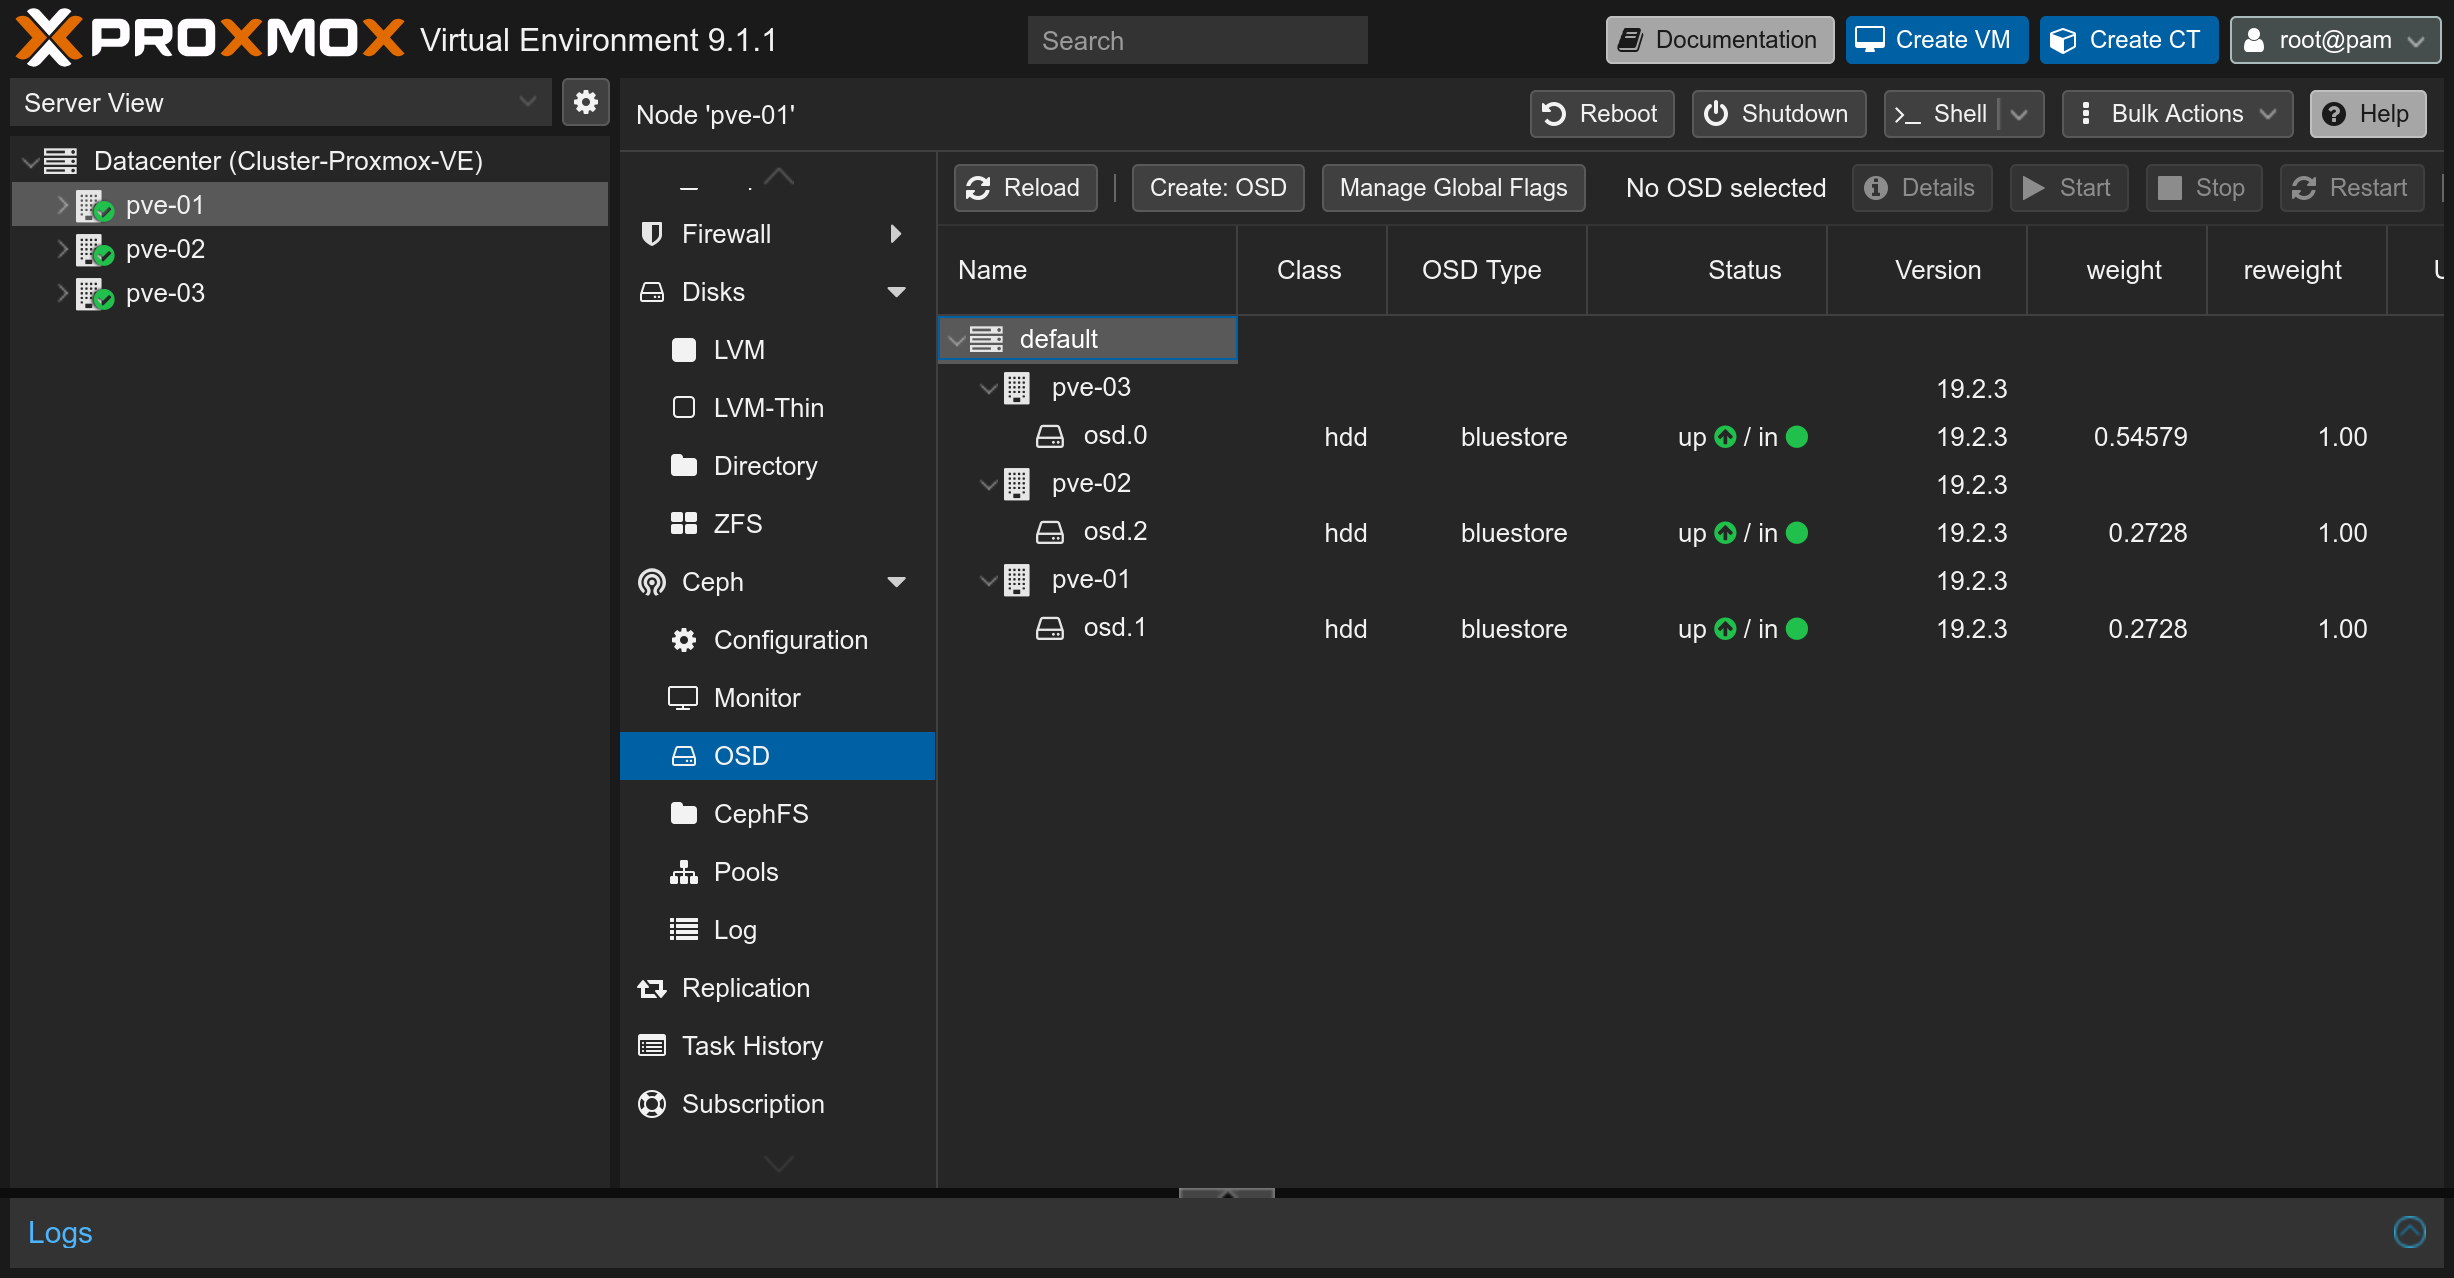
\includegraphics[width=0.9\textwidth]{image/ch4/ceph osd.png}
    \caption{État du cluster Ceph montrant les MON, OSD et le pool RBD}
    \label{fig:ceph-health-ok}
\end{figure}
\begin{figure}[H]
    \centering
    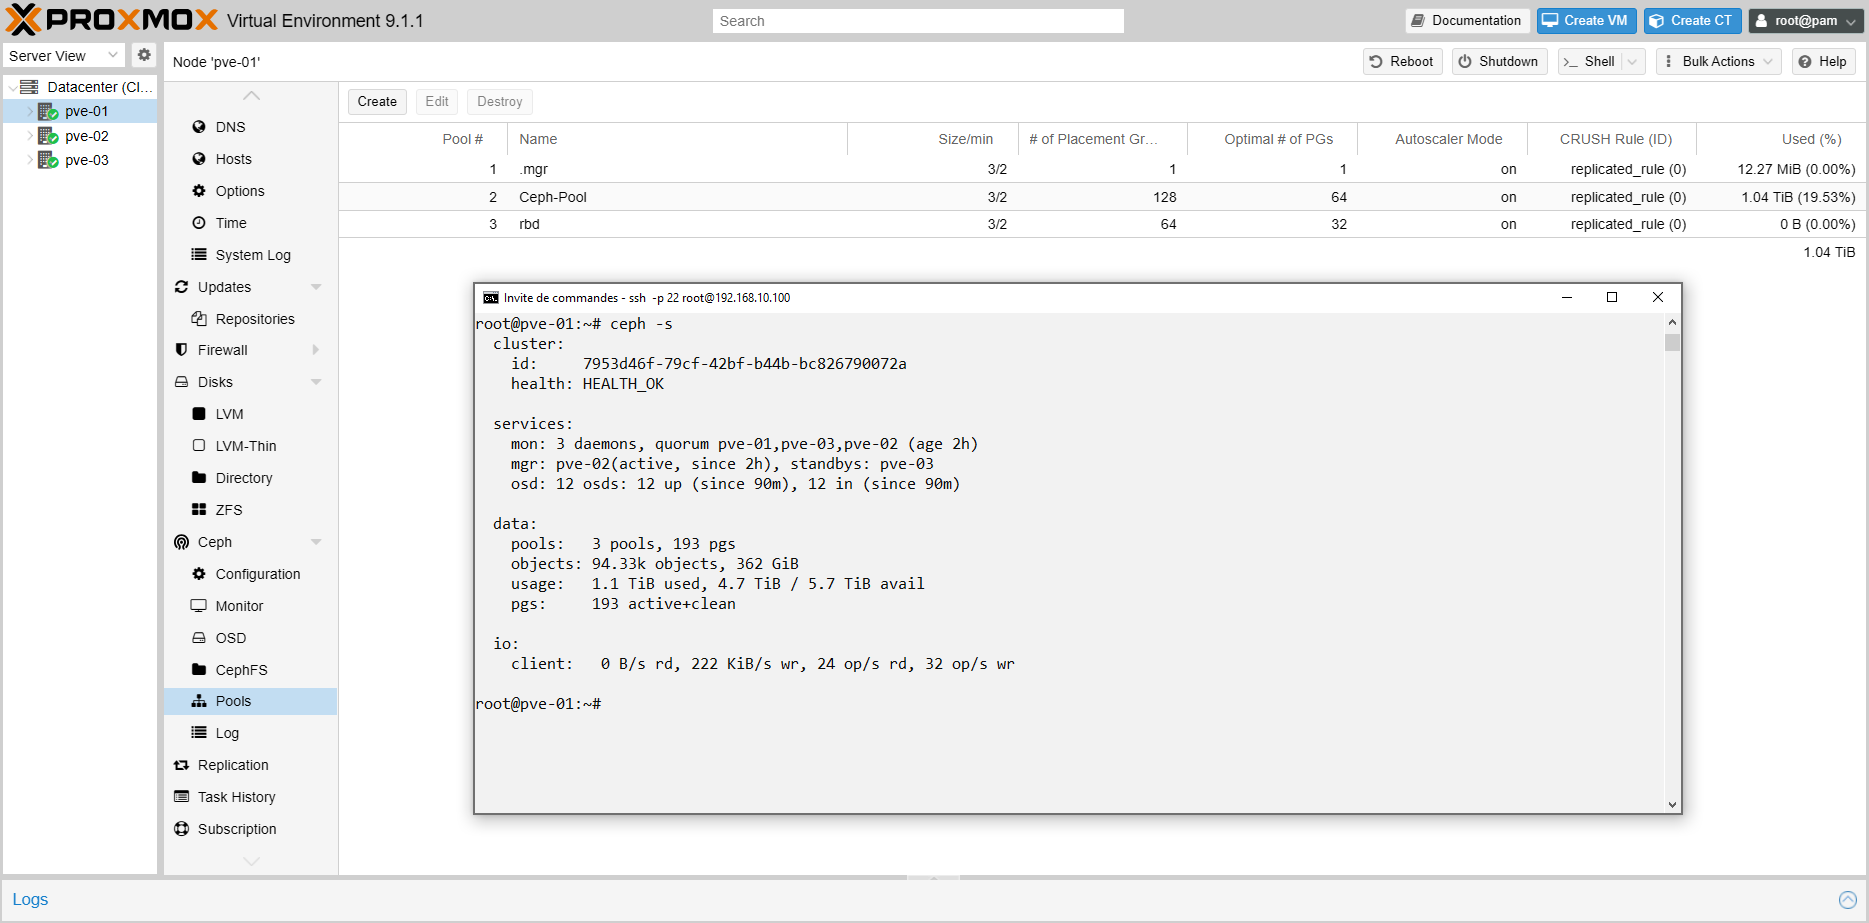
\includegraphics[width=0.9\textwidth]{image/ch4/ceph pool health.png}
    \caption{État du cluster Ceph montrant les MON, OSD et le pool RBD}
    \label{fig:ceph-health-ok}
\end{figure}

{\color{bleuu} \subsection{Validation de la tolérance aux pannes}}

\par La tolérance aux pannes de la couche stockage a été vérifiée par un scénario de panne simulée. Lors de l’extinction d’un nœud, le cluster Ceph est passé temporairement à l’état \texttt{HEALTH\_WARN}, mais les données sont restées accessibles grâce au facteur de réplication.\\

\par Après le retour du nœud défaillant, Ceph a automatiquement lancé la resynchronisation des données et l’état du cluster est revenu à \texttt{HEALTH\_OK}. Ce test valide le bon comportement de la couche stockage distribuée.\\

{\color{bleu} \section{Partie III --- Couche Réseau}}

{\color{bleuu} \subsection{Configuration Open vSwitch et tunnels VxLAN}}

{\color{bleuuu} \subsubsection{Installation d’Open vSwitch}}

\par Open vSwitch a été installé sur chaque nœud Proxmox afin de construire une couche réseau virtuelle flexible, adaptée au transport de plusieurs flux logiques sur le même réseau physique.\\

\begin{lstlisting}[style=sonacode,language=bash,caption={Installation d’Open vSwitch},label={lst:ovs-install}]
apt install openvswitch-switch
\end{lstlisting}

\par Un bridge principal a été créé sur chaque nœud, puis l’interface physique principale y a été attachée pour servir de point de transit à tous les tunnels VxLAN.\\

\begin{lstlisting}[style=sonacode,language=bash,caption={Création du bridge OVS principal},label={lst:ovs-create-bridge}]
ovs-vsctl add-br vmbr1
ovs-vsctl add-port vmbr1 eno1
\end{lstlisting}

{\color{bleuuu} \subsubsection{Configuration complète des interfaces sur PVE-01}}

\par Le fichier \texttt{/etc/network/interfaces} du nœud PVE-01 centralise l’ensemble de la configuration réseau, y compris le bridge principal, les interfaces VXLAN point-à-point vers les autres nœuds, les interfaces internes OVS, et les bridges Linux utilisés pour connecter les machines virtuelles.\\

\begin{lstlisting}[style=sonacode,language={},caption={Configuration réseau complète de PVE-01},label={lst:pve01-full-interfaces}]
auto lo
iface lo inet loopback

iface nic0 inet manual

auto vmbr0
iface vmbr0 inet static
    address 192.168.10.100/24
    gateway 192.168.10.36
    ovs_type OVSBridge
    ovs_ports nic0

auto nic0
iface nic0 inet manual
    ovs_type OVSPort
    ovs_bridge vmbr0

iface nic1 inet manual
iface nic2 inet manual
iface nic3 inet manual

# ===== COROSYNC VXLAN =====
auto vxlan20-pve02
iface vxlan20-pve02 inet manual
    ovs_type OVSPort
    ovs_bridge vmbr0
    ovs_options type=vxlan options:remote_ip=192.168.10.213 options:key=20

auto vxlan20-pve03
iface vxlan20-pve03 inet manual
    ovs_type OVSPort
    ovs_bridge vmbr0
    ovs_options type=vxlan options:remote_ip=192.168.10.84 options:key=20

auto vxlan20-int
iface vxlan20-int inet static
    address 10.10.20.1/24
    ovs_type OVSIntPort
    ovs_bridge vmbr0

# ===== CEPH VXLAN =====
auto vxlan30-pve02
iface vxlan30-pve02 inet manual
    ovs_type OVSPort
    ovs_bridge vmbr0
    ovs_options type=vxlan options:remote_ip=192.168.10.213 options:key=30

auto vxlan30-pve03
iface vxlan30-pve03 inet manual
    ovs_type OVSPort
    ovs_bridge vmbr0
    ovs_options type=vxlan options:remote_ip=192.168.10.84 options:key=30

auto vxlan30-int
iface vxlan30-int inet static
    address 10.10.30.1/24
    ovs_type OVSIntPort
    ovs_bridge vmbr0

# ===== VXLAN 40 (Ceph Public) =====
auto vxlan40-pve02
iface vxlan40-pve02 inet manual
    ovs_type OVSPort
    ovs_bridge vmbr0
    ovs_options type=vxlan options:remote_ip=192.168.10.213 options:key=40

auto vxlan40-pve03
iface vxlan40-pve03 inet manual
    ovs_type OVSPort
    ovs_bridge vmbr0
    ovs_options type=vxlan options:remote_ip=192.168.10.84 options:key=40

auto vxlan40-int
iface vxlan40-int inet static
    address 10.10.40.1/24
    ovs_type OVSIntPort
    ovs_bridge vmbr0

# ===== VXLAN 50 (Migration) =====
auto vxlan50-pve02
iface vxlan50-pve02 inet manual
    ovs_type OVSPort
    ovs_bridge vmbr0
    ovs_options type=vxlan options:remote_ip=192.168.10.213 options:key=50

auto vxlan50-pve03
iface vxlan50-pve03 inet manual
    ovs_type OVSPort
    ovs_bridge vmbr0
    ovs_options type=vxlan options:remote_ip=192.168.10.84 options:key=50

auto vxlan50-int
iface vxlan50-int inet static
    address 10.10.50.1/24
    ovs_type OVSIntPort
    ovs_bridge vmbr0

# ===== VXLAN 90 (Backup) =====
auto vxlan90-pve02
iface vxlan90-pve02 inet manual
    ovs_type OVSPort
    ovs_bridge vmbr0
    ovs_options type=vxlan options:remote_ip=192.168.10.213 options:key=90

auto vxlan90-pve03
iface vxlan90-pve03 inet manual
    ovs_type OVSPort
    ovs_bridge vmbr0
    ovs_options type=vxlan options:remote_ip=192.168.10.84 options:key=90

auto vxlan90-int
iface vxlan90-int inet static
    address 10.10.90.1/24
    ovs_type OVSIntPort
    ovs_bridge vmbr0

# ===== VXLAN 60 =====
auto vxlan60-pve02
iface vxlan60-pve02 inet manual
    ovs_type OVSPort
    ovs_bridge vmbr0
    ovs_options type=vxlan options:remote_ip=192.168.10.213 options:key=60

auto vxlan60-pve03
iface vxlan60-pve03 inet manual
    ovs_type OVSPort
    ovs_bridge vmbr0
    ovs_options type=vxlan options:remote_ip=192.168.10.84 options:key=60

auto vxlan60-int
iface vxlan60-int inet static
    ovs_type OVSIntPort
    ovs_bridge vmbr0

# ===== VXLAN 70 (Dev) =====
auto vxlan70-pve02
iface vxlan70-pve02 inet manual
    ovs_type OVSPort
    ovs_bridge vmbr0
    ovs_options type=vxlan options:remote_ip=192.168.10.213 options:key=70

auto vxlan70-pve03
iface vxlan70-pve03 inet manual
    ovs_type OVSPort
    ovs_bridge vmbr0
    ovs_options type=vxlan options:remote_ip=192.168.10.84 options:key=70

auto vxlan70-int
iface vxlan70-int inet static
    ovs_type OVSIntPort
    ovs_bridge vmbr0

# ===== VXLAN 80 (DMZ) =====
auto vxlan80-pve02
iface vxlan80-pve02 inet manual
    ovs_type OVSPort
    ovs_bridge vmbr0
    ovs_options type=vxlan options:remote_ip=192.168.10.213 options:key=80

auto vxlan80-pve03
iface vxlan80-pve03 inet manual
    ovs_type OVSPort
    ovs_bridge vmbr0
    ovs_options type=vxlan options:remote_ip=192.168.10.84 options:key=80

auto vxlan80-int
iface vxlan80-int inet static
    ovs_type OVSIntPort
    ovs_bridge vmbr0

# ===== VM Bridges =====
auto vmbr60
iface vmbr60 inet manual
    bridge_ports vxlan60-int
    bridge_stp off
    bridge_fd 0

auto vmbr70
iface vmbr70 inet manual
    bridge_ports vxlan70-int
    bridge_stp off
    bridge_fd 0

auto vmbr80
iface vmbr80 inet manual
    bridge_ports vxlan80-int
    bridge_stp off
    bridge_fd 0

source /etc/network/interfaces.d/*
\end{lstlisting}

\par Cette architecture permet de transporter plusieurs réseaux logiques isolés sur le même réseau physique sans dépendre d’un switch physique configuré en VLAN.\\

\begin{table}[H]
\centering
\caption{Résumé des VxLAN utilisés dans l’infrastructure}
\begin{tabular}{|c|l|l|}
\hline
\textbf{VNI} & \textbf{Usage} & \textbf{Réseau} \\
\hline
20 & Corosync / Heartbeat & 10.10.20.0/24 \\
\hline
30 & Ceph Cluster & 10.10.30.0/24 \\
\hline
40 & Ceph Public & 10.10.40.0/24 \\
\hline
50 & Live Migration & 10.10.50.0/24 \\
\hline
60 & Réseau Dev & 172.16.60.0/24 \\
\hline
70 & Réseau Prod & 172.16.70.0/24 \\
\hline
80 & Réseau DMZ & 172.16.80.0/24 \\
\hline
90 & Backup & 10.10.90.0/24 \\
\hline
\end{tabular}
\end{table}

{\color{bleuu} \subsection{Déploiement de la VM OPNsense}}

{\color{bleuuu} \subsubsection{Création et interfaces réseau}}

\par OPNsense a été déployé sous forme de machine virtuelle sur le cluster Proxmox. Son disque système est stocké sur le pool Ceph, ce qui permet de bénéficier du stockage distribué et de la haute disponibilité.\\

\par La VM dispose de 4 Go de RAM, de 2 vCPUs et d’un disque de 20 Go. Quatre interfaces réseau lui ont été attribuées afin de jouer le rôle de routeur et pare-feu pour les différents segments de l’infrastructure.\\

\begin{table}[H]
\centering
\caption{Interfaces de la VM OPNsense}
\begin{tabular}{|l|l|l|l|}
\hline
\textbf{Interface VM} & \textbf{Bridge Proxmox} & \textbf{Rôle} & \textbf{Adresse IP} \\
\hline
net0 (em0) & vmbr0 & WAN & 192.168.10.65/24 \\
\hline
net1 (em1) & vmbr60 & LAN Dev & 172.16.60.1/24 \\
\hline
net2 (em2) & vmbr70 & LAN Prod & 172.16.70.1/24 \\
\hline
net3 (em3) & vmbr80 & LAN DMZ & 172.16.80.1/24 \\
\hline
\end{tabular}
\end{table}

\begin{figure}[H]
    \centering
    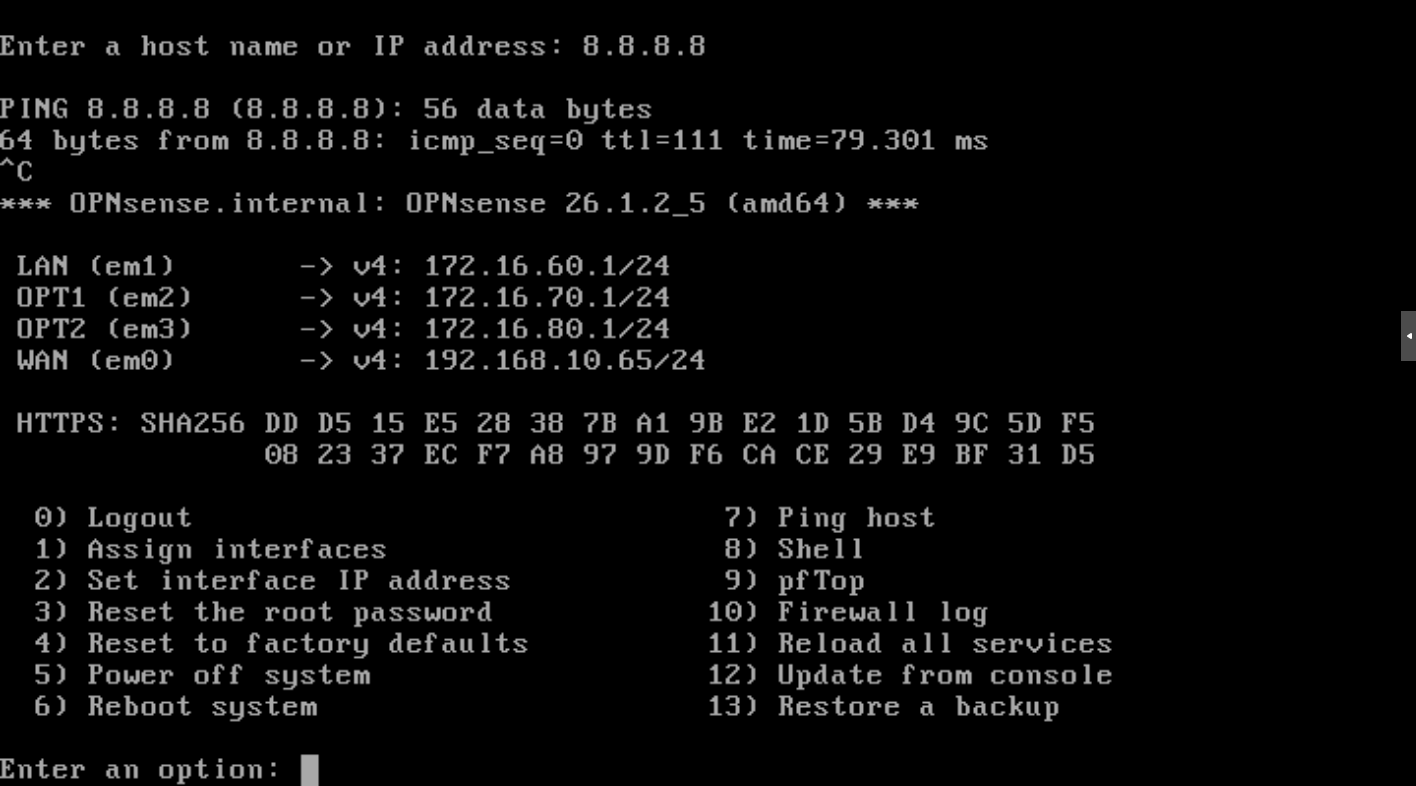
\includegraphics[width=0.9\textwidth]{image/ch4/opnsense.png}
    \caption{Configuration des interfaces de la VM OPNsense}
    \label{fig:opnsense-interfaces}
\end{figure}

{\color{bleuuu} \subsubsection{NAT sortant}}

\par Le NAT sortant automatique a été activé dans OPNsense afin de permettre aux réseaux internes de sortir vers Internet via l’interface WAN. Cette configuration a simplifié le routage pour les VMs hébergées sur les réseaux Dev, Prod et DMZ.\\

{\color{bleuu} \subsection{Configuration du service DHCP}}

\par Le service DHCP a été activé via \texttt{dnsmasq} sur les interfaces LAN internes. Ce choix a été retenu car il est simple à configurer et convient bien à un environnement de laboratoire.\\

\begin{table}[H]
\centering
\caption{Plages DHCP configurées sur OPNsense}
\begin{tabular}{|l|l|l|l|}
\hline
\textbf{Interface} & \textbf{Plage début} & \textbf{Plage fin} & \textbf{Gateway} \\
\hline
LAN (Dev) & 172.16.60.10 & 172.16.60.250 & 172.16.60.1 \\
\hline
OPT1 (Prod) & 172.16.70.10 & 172.16.70.250 & 172.16.70.1 \\
\hline
OPT2 (DMZ) & 172.16.80.10 & 172.16.80.250 & 172.16.80.1 \\
\hline
\end{tabular}
\end{table}

\par Le bon fonctionnement de DHCP a été vérifié par une capture réseau sur l’interface LAN d’OPNsense pendant le démarrage d’une VM de test.\\

\begin{lstlisting}[style=sonacode,language=bash,caption={Capture du trafic DHCP avec tcpdump},label={lst:tcpdump-dhcp}]
tcpdump -i em1 port 67 or port 68
\end{lstlisting}

\par Cette vérification a montré le cycle normal des échanges DHCP, depuis le \textit{Discover} jusqu’au \textit{Offer}, puis l’attribution effective de l’adresse IP à la machine virtuelle.\\

{\color{bleuu} \subsection{Validation de la haute disponibilité réseau et applicative}}

\par Un scénario de panne a été réalisé afin de tester le comportement global de l’infrastructure en cas de perte d’un nœud physique. L’arrêt brutal de PVE-01 a permis d’observer la détection de panne par Corosync, le redémarrage des services protégés sur un autre nœud, puis la resynchronisation automatique après le retour du serveur.\\

\par Cette séquence a montré que le cluster restait opérationnel malgré la défaillance, et que les mécanismes de haute disponibilité répondaient correctement à ce type d’événement.\\

\begin{figure}[H]
    \centering
    \fbox{\rule{0pt}{6cm}\rule{0.9\textwidth}{0pt}}
    \caption{Chronologie des événements lors d’une panne d’un nœud physique}
    \label{fig:ha-failure-sequence}
\end{figure}

{\color{bleu} \section{Conclusion}}

\par Ce chapitre a présenté l’implémentation réelle de l’infrastructure hyperconvergée open source mise en place dans le cadre du projet. La couche calcul a permis de déployer Proxmox, le cluster, le monitoring, l’automatisation et les services applicatifs. La couche stockage a été assurée par Ceph avec réplication et tolérance aux pannes. Enfin, la couche réseau a été construite avec Open vSwitch, les tunnels VxLAN, OPNsense et les services d’adressage associés.\\

\par Les différents tests réalisés ont confirmé la cohérence de l’architecture proposée et sa capacité à répondre aux objectifs du projet dans un environnement de laboratoire structuré. Le chapitre suivant présentera l’évaluation des performances obtenues ainsi qu’une analyse des résultats expérimentaux.\\
\end{justify}

\end{document}
